\documentclass[12pt]{report} 
\usepackage[main=english, italian]{babel}
\usepackage[utf8]{inputenc}  
\usepackage[autostyle, english = american]{csquotes}
\usepackage{graphicx} % Required for inserting images
\usepackage[hidelinks]{hyperref}
\urlstyle{sf}
\usepackage[nottoc]{tocbibind}  
\usepackage{verbatim} %Package per i commenti
\usepackage[a4paper, left=2.8cm, right=2.8cm, top=2cm, bottom=2cm]{geometry}
\usepackage{subcaption}
\usepackage[none]{hyphenat} 
\usepackage[T1]{fontenc}     
\usepackage{lmodern}         
\usepackage{microtype} 
\usepackage{biblatex} 
\usepackage{float}  
\usepackage{pgfplots}
\pgfplotsset{compat=1.18}
\usepackage{pgfplotstable}  
\usepackage{booktabs}
\usepackage{caption}
\usepackage{placeins}
\usepackage{pgffor} % for \foreach
\usepackage{pdfpages}
\usepackage{regexpatch}
\usepackage{xstring}


\begin{document}
\sloppy
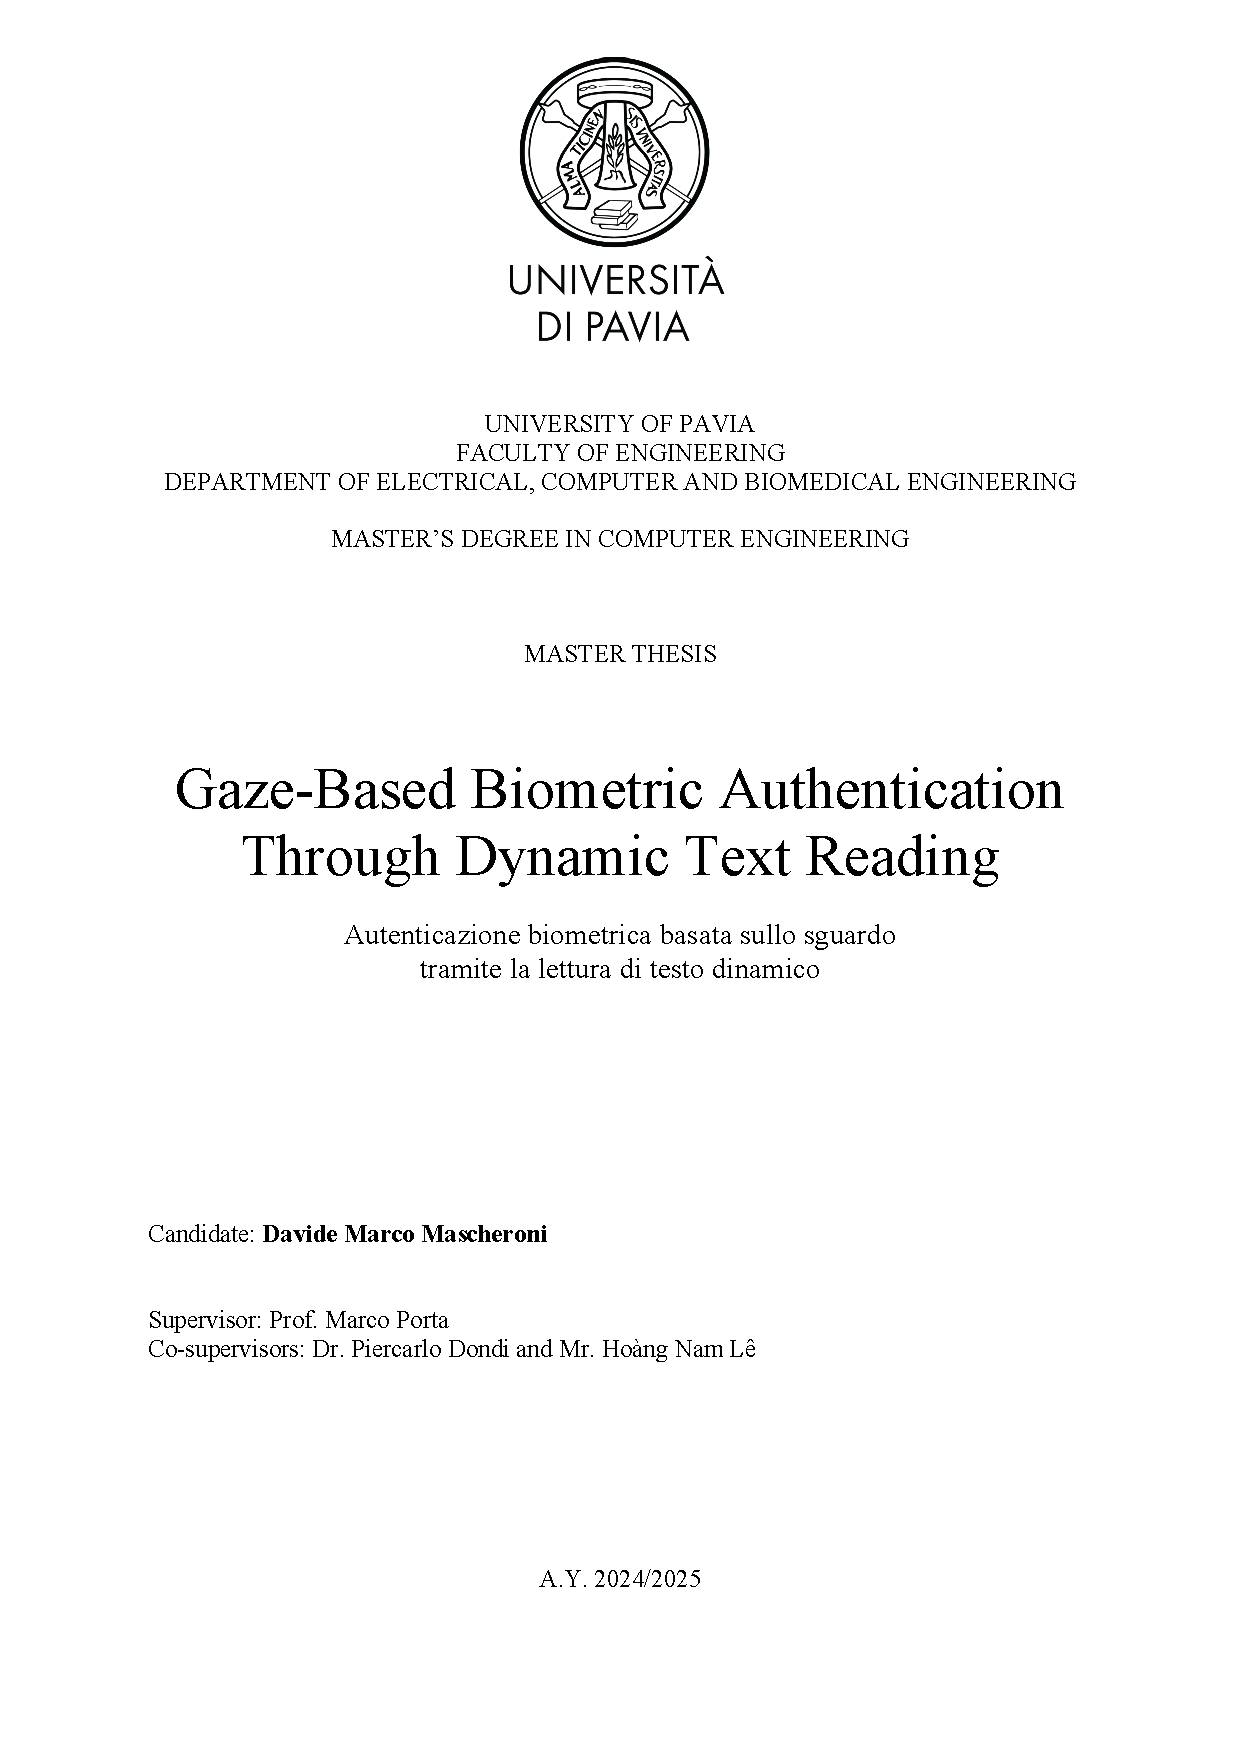
\includepdf[pages=1, fitpaper=true]{Images/Theory/Frontespizio.pdf}


\newpage
\renewcommand{\contentsname}{Table of contents}
\tableofcontents
\newpage

\begin{abstract}
\setlength{\parindent}{0pt}
\setlength{\parskip}{0.7\baselineskip}
\noindent
In recent years, the technological landscape has advanced rapidly, enabling individuals to access portable devices such as personal computers and smartphones.
While this evolution has greatly simplified many aspects of daily life, it has also introduced new and significant security challenges, particularly in the domain of user authentication.
To address these concerns, this work proposes a novel approach grounded in the field of behavioral biometrics, aimed at providing an additional layer of security for personal devices.
The goal of the proposed method is not to replace conventional authentication techniques, such as PIN codes or physiological biometric systems, but rather to complement them with an additional behavioral verification mechanism.

Specifically, this study investigates gaze-based soft biometrics using simple dynamic text animations as visual stimuli.
Two types of text movement are explored: a vertical block of text moving from bottom to top, and a horizontal scrolling line of text moving from left to right.
Each animation type is further varied by combining two display speeds and two font sizes, resulting in a total of eight distinct dynamic text stimuli.
Importantly, the proposed method does not require any preliminary calibration of the eye-tracking device, ensuring ease of deployment.

Experimental data were collected from 35 participants, and subsequently analyzed through a series of machine learning algorithms addressing both identification and verification tasks.
The obtained results are highly encouraging for both applications.
In the identification scenario, the system achieved an accuracy of 82.86\% using a single animation stimulus.
In the verification task, which represents the primary use case for soft biometric systems, the best performance reached an accuracy of 92.2\% with an Equal Error Rate (EER) of 3.6\%.
\end{abstract}

\begin{otherlanguage}{italian}
  \renewcommand{\abstractname}{Sommario}
  \begin{abstract}
  \setlength{\parindent}{0pt}
  \setlength{\parskip}{0.7\baselineskip}
  \noindent
  Negli ultimi anni, il panorama tecnologico è avanzato rapidamente, consentendo agli individui di accedere a dispositivi portatili come computer personali e smartphone.
  Sebbene questa evoluzione abbia notevolmente semplificato molti aspetti della vita quotidiana, ha anche introdotto nuove e significative sfide in termini di sicurezza, in particolare nel campo dell’autenticazione degli utenti.
  Per affrontare queste problematiche, questo lavoro propone un approccio innovativo basato sulla disciplina delle biometrie comportamentali, con l’obiettivo di fornire un ulteriore livello di sicurezza per i dispositivi personali.
  Lo scopo del metodo proposto non è sostituire le tecniche di autenticazione convenzionali, come i codici PIN o i sistemi biometrici fisiologici, bensì affiancarle con un meccanismo di verifica comportamentale aggiuntivo.

  In particolare, questo studio indaga l’uso di biometrie comportamentali basate sullo sguardo (gaze-based soft biometrics) impiegando semplici animazioni di testo dinamico come stimoli visivi.
  Sono stati esplorati due tipi di movimento del testo: un blocco verticale di testo che si muove dal basso verso l’alto e una linea orizzontale scorrevole che si muove da sinistra a destra.
  Ciascun tipo di animazione è stato ulteriormente variato combinando due velocità di scorrimento e due dimensioni dei caratteri, per un totale di otto differenti stimoli di testo dinamico.
  È importante sottolineare che il metodo proposto non richiede alcuna calibrazione preliminare del dispositivo di eye tracking, garantendo così una maggiore semplicità di utilizzo.

  I dati sperimentali sono stati raccolti da 35 partecipanti e successivamente analizzati mediante una serie di algoritmi di apprendimento automatico applicati ai compiti di identificazione e verifica.
  I risultati ottenuti sono molto incoraggianti per entrambe le applicazioni.
  Nel caso dell’identificazione, il sistema ha raggiunto una accuratezza dell’82.86\% utilizzando un singolo stimolo di animazione.
  Nel compito di verifica, che rappresenta l’applicazione principale dei sistemi biometrici comportamentali, la migliore prestazione ha raggiunto una accuratezza del 92.2\% con un EER del 3.6\%.
  \end{abstract}
\end{otherlanguage}
\newpage

\chapter{Introduction}

\setlength{\parindent}{0pt}
\setlength{\parskip}{0.7\baselineskip}
In recent years, new information technologies have become increasingly widespread in everyday life. 
Initially, the most prominent example was the personal computer, which revolutionized the way individuals work, communicate, and access information.
However, technological development has progressed rapidly, and today there is a wide variety of smart devices available on the market.
Such technologies encompass tablets, wearable devices, and home automation systems, with mobile phones representing the most prominent example.
According to Statista [1], in 2024 more than 7.2 billion people worldwide own a smartphone, making it one of the most ubiquitous devices in human history.
The growing reliance on such devices has brought tremendous convenience but also introduced significant security challenges. 
Mobile devices store and process sensitive personal information, such as banking details, private communications, and location history. 
This makes them prime targets for cyberattacks, and without adequate protection, they could be exploited for identity theft, financial fraud, and unauthorized access to personal data.
To address these risks, multiple layers of security have been developed for mobile devices, including passwords, PINs, fingerprint scans, and facial recognition.
However, these traditional methods often have limitations, such as being susceptible to theft, spoofing, or user inconvenience. 

This thesis focuses on a more advanced and promising approach: behavioral biometrics.
Behavioral biometrics examine the distinctive ways in which users interact with a device, enabling continuous identity verification.
This approach provides user authentication in a less intrusive way, but unfortunatelly it doesn't reach the accuracy of the traditional biometric approach.
For this reason behavioral biometric is rarely used as the main approach for user identification, but instead represents an additional layer of security to build on top of the traditional approaches.

This thesis includes a chapter dedicated to the foundations of behavioral biometrics, providing a comprehensive overview of this field and its relationship with traditional biometric approaches.
In particular, the discussion highlights the distinctive features that separate behavioral biometrics from more conventional physiological methods.
Behavioral biometrics are based on human actions and responses, whereas traditional approaches rely on physical characteristics such as fingerprints or facial recognition.
Furthermore, several real-world applications are examined, illustrating how behavioral biometrics are already integrated into everyday technologies. 
Although these examples do not directly concern gaze-based systems, which constitute the focus of the present research, they demonstrate the growing importance and versatility of this emerging discipline.

The subsequent chapter traces the historical development of visual attention studies, which represent a key theoretical foundation for gaze-based biometrics. 
Understanding how visual attention operates helps explain why recording gaze data is so meaningful and how it can reveal a person’s cognitive and attentional patterns. 
To support this understanding, a brief section is dedicated to the anatomy of the human eye and the mechanisms underlying its movements. 
Particular emphasis is placed on saccades and fixations, as these represent the fundamental components of gaze behavior captured during eye-tracking experiments.

The chapter then introduces the eye tracker, the instrument that enables precise measurement of where and how a user focuses attention during a visual task. 
Various eye-tracking technologies are presented, with specific attention given to the corneal reflection–based system, which is also employed in this study.

No scientific investigation would be complete without situating it within the context of prior research. 
For this reason, a dedicated chapter is devoted to a review of the related work in the area of gaze-based biometrics. 
This field aims to exploit individual differences in gaze behavior to achieve reliable user authentication. 
The review discusses a wide range of methodological approaches, including systems inspired by ATM authentication processes, studies focusing on fixation and scanpath analysis, and works based on gaze velocity, pupil size, oculomotor dynamics, and head orientation.
Through this discussion, the chapter outlines the evolution of gaze-based biometric research and clarifies the position and originality of the present study within this scientific landscape.

After this theoretical introduction, we move to the core of the project, which consists of an experiment focused on gaze-based biometrics using dynamic text as stimuli.
A total of 35 participants took part in the study, each completing three trials per day, repeated over three different days, for a total of nine trials per participant.
During each trial, participants were seated in front of a monitor on which a series of animations were displayed, while an eye tracker recorded their gaze behavior.
The experimental stimuli consisted of two types of animations: a vertical block of text moving from the bottom to the top of the screen, and a horizontal scrolling line of text moving from left to right.
Each of these animations was presented with two different speeds and two font sizes, resulting in a total of eight distinct stimuli.

To proceed, a machine learning analysis is conducted using the previously constructed database, focusing on the tasks of identification and verification.
The objective is to assess system performance across both tasks and identify the best-performing animation for potential real-world deployment.
The first part of the analysis focuses on identification, formulated as a multiclass classification problem. 

This evaluation is initially conducted using the complete dataset, followed by a detailed examination of each individual animation, which represents the primary focus of this study.
The initial identification phase demonstrated the discriminative potential of gaze patterns elicited by these stimuli, achieving up to 67.6\% accuracy with an MLP classifier under session-based evaluation. 
Following this, the analysis proceeded with the evaluation of each individual animation, tested under two distinct training modalities: Single Train (ST) and Full Train (FT). 
The highest performance in this phase was obtained with the ST configuration using the VB\_FA\_BIG animation, achieving an accuracy of 82.86\% with the SVC classifier. 
These results indicate that this animation can be effectively employed in identification scenarios where such a level of accuracy meets the application’s requirements.

Subsequently, the analysis proceeds with the verification phase, which forms the central part of the study and provides the most complete assessment of the proposed gaze-based biometric system.
The analysis explores several experimental configurations that vary in training modality (Single Train and Full Train), evaluation strategy (best-model and pairwise), and testing condition (closed-set, open-set, and reduced recording durations).
A dedicated chapter is presented for each experimental configuration, detailing the methodology, results, and comparative discussion for every combination of training modality, evaluation strategy, and testing condition.

Overall, the best verification performance was achieved using the VB\_FA\_SMA animation under the Full Train configuration and best-model evaluation, reaching an accuracy of 92.6\% and an EER of 4\%.
The lowest EER, however, was obtained in the Single Train setup with the VB\_FA\_BIG animation, achieving 3.6\% EER and 92.2\% accuracy with the Random Forest classifier.
In the open-set scenario, the system maintained strong performance, with the VB\_FA\_SMA animation and SVC classifier reaching 91.9\% accuracy and 6.1\% EER.
When the recording duration was reduced, results remained robust.
For 10-second recordings, the VB\_FA\_SMA animation achieved 92.7\% accuracy and 5.4\% EER using the Full Train configuration, while for 5-second recordings, it reached 90.6\% accuracy and 6.4\% EER with the NuSVC classifier.

To conclude, a comparative analysis between dynamic and static text stimuli is presented.
For this study, a similar data collection protocol was followed, consisting of three sessions of three trials each.
Eight participants were involved to evaluate and compare the performance of the two methods.
In terms of quantitative performance, the highest results for dynamic text in the verification task were achieved using the MLP classifier, reaching an accuracy of 92.19\% with an EER of 6.77\%.
By comparison, static text stimuli obtained an accuracy of 87.5\%, also with MLP, but with a lower EER of 4.17\%.
These results highlight a trade-off between robustness and precision: dynamic text offers greater consistency across sessions, while static text provides improved reliability in terms of error rate.
Additionally, vertical block–based animations consistently outperformed horizontal scroll–based ones across nearly all experimental conditions, indicating their stronger suitability for gaze-based biometric applications.

\newpage

\chapter{Behavioral Biometric}

\noindent
As per Jim Holdsworth et al. [88] Behavioral biometrics is a form of authentication that analyzes the unique patterns in a user's activity to verify their identity. 
In particular this discipline is able to collect, in a non intrusive way, a distinctive way in which a user achieve a task.
As we said earlier this technique achieve low performance to be used as the only authentication method in a system, so it is used as a complement of more secure solutions.
This additional level of security will focus only on a verification purpose to detect possible attacks or fraud.
A major advantage over traditional PIN or password-based methods is that mimicking the genuine user's behavioral patterns to gain system access is considerably more difficult.
These advantages have contributed to the growing prominence of the field, which has attracted considerable research attention in recent years.

\section{Identification vs Verification}

An important thing to mention is surely the difference between identification and verification.
In fact, this difference represents the basis through which various biometric technologies have been developed.

Identification is the process by which a subject is identified, based on some characteristics that it possesses, from a large number of other subjects.
Identification establishes a user's identity based on the information they provide. 
This can include a username, email address, or any other information that uniquely identifies them.
The problem is used do address the question: "Who are you?"[114]

Verification is the process by which a machine can verify the correct identity of a subject.
In particular a user can only be accepted or rejected, but not recognized over a large number of users.
Verification confirms that the user is who they claim to be [114] by comparing the information provided by the user against a trusted source, such as a government-issued ID, a passport, or a driver's license.


\section{Biometric based on identification}

The most well-known biometric technologies are those based on iris recognition and fingerprint scanning. 
Unlike traditional passwords, which identify a user through information they know, these technologies rely on intrinsic physical characteristics of the individual.
They were specifically developed with the goal of user identification.

Fingerprints are a unique feature that every person has, and can be used to distinguish a person between every other subjects. 
Biometrics uses the fingerprint to identify and authenticate a person.
First, the subject places their finger on a scanner which will be able to save the fingerprint as a biometric profile.
This, unless there are particular accidents in the user's life, will remain the same until death.
After this first step we will move on to the authentication phase.
In this phase the subject will place their finger on the scanner again, which will take the biometric data and compare them with those saved in the previous step.
The outcome of this procedure will be the authentication and identification of a user by the system if the data are matching and a reject if the data differs between them.

Biometric iris recognition uses the intrinsic composition of the human eye to authenticate and identify someone.
The process is similar to that of a fingerprint, with some minor differences in the scanner used to create the biometric profile of a subject.

\begin{figure}[htbp]
    \centering
    \begin{subfigure}[t]{0.45\textwidth}
        \centering
        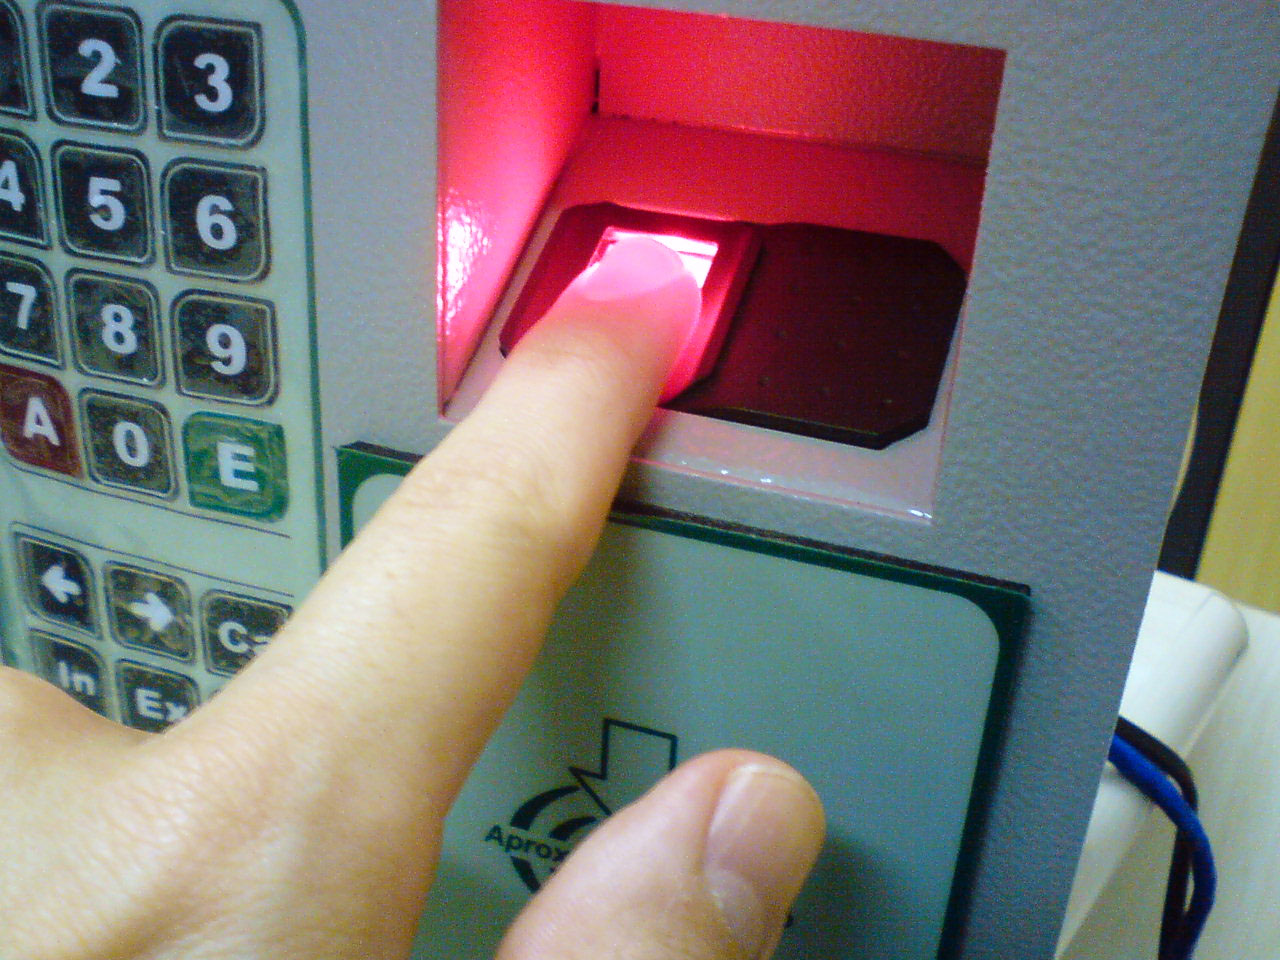
\includegraphics[width=\linewidth]{Images/Theory/Fingerprint_scanner_identification.jpg}
        \caption{Scanner for fingerprint.}
        \label{fig:scanner_fingerprint}
    \end{subfigure}
    \hfill
    \begin{subfigure}[t]{0.45\textwidth}
        \centering
        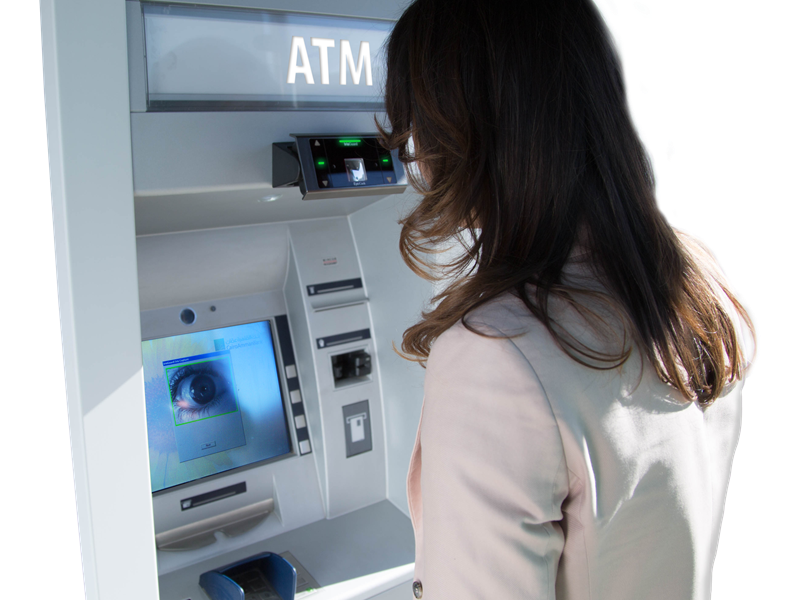
\includegraphics[width=\linewidth]{Images/Theory/eye.png}
        \caption{Scanner for iris recognition.}
        \label{fig:scanner_eye}
    \end{subfigure}
    \caption{Different type of scanner.}
    \label{fig:scanners}
\end{figure}

The figure \ref{fig:scanners} shows a real world example of scanners used for fingerprint and iris authentication and identification.

As per Nist [2] the best fingerprint systems can reach an accuracy of more than 99\%.
In particular, their test used operational fingerprints from a variety of U.S. and state government sources. 
A total of 48,105 fingerprint sets from 25,309 individuals, comprising 393,370 distinct fingerprint images, were used in the test.
The performance was based on how many fingerprint images of a person are matched.
The best system was accurate 98.6 percent of the time on single-finger tests, 99.6 percent of the time on two-finger tests, and 99.9 percent of the time for tests involving four or more fingers.
These results were obtained for a false positive rate of 0.01\%, which indicates the people who should have been rejected but were instead accepted by the system.

For what concern the accuracy of iris recognition a Nec [3] study set a benchmark of 99.58\% accuracy.
This study was performed for a 1:N identification problem and it included over 500.000 participants, using both of their eyes for the trial.

As we expected these technology are very strong and reliable because are built over some intrinsic characteristic of a subject.
These characteristics can be used to uniquely identify a person and remain unchanged throughout life.
Another advantage is also that, unlike password-based systems, the user does not have to remember secret information.
Furthermore, it is more difficult to try to authenticate using another person's fingerprint or iris compared to a system based on what a subject knows.

\section{Behavioral biometric}

Behavioral biometrics is a discipline primarily focused on the verification problem.
Unlike physical biometrics, it does not rely on inherent physical characteristics, but rather on a person's behavior. 
Each individual behaves differently, using specific skills or strategies to accomplish tasks in everyday life.
So the machine will be able to collect information about how a subject behave and it will be able to tell us if the user is really who is claiming to be.
As we can expected the behavior is a soft biometric and less robust compared to the fingerprint or iris recognition.
In fact this technology is not used in substitution of the former biometric system, but will be used as another security layer to verify the identity of a subject.
In comparison to the former biometry the system can collect the data in a non intrusive way, without the user even realizing it, and it doesn't need an expensive hardware to do so.

As per Behavioral Biometrics for Human Identification: Intelligent Applications [4] behavioral biometric can be classified in five different categories based on the information about the user being collected:
\begin{itemize}
    \item Authorship based biometric: Is used to collect something that a user produce like a drawing or a written text. 
    Based on this the system will be able to recognize some particular characteristics about the style and verify a subject.
    \item Human Computer Interaction: Every user has a distinctive behavior when interact directly with a machine. 
    The most famous method to do so is certainly the keyboard and the mouse. 
    The way in which the user perform these actions is used as a method for verification.
    \item Indirect HCI-based biometrics: This method is related to the second point, so the interaction of a user with a machine.
    The goal is to use what the users leaves during the interaction, as an indirect information, to verify it. 
    Some examples of indirect information are audit log, program execution traces and memory usage.
    \item Motor skills: This is probably the best research group because it is based on some characteristic that the user have and learn during his life.
    The motor skill indicate the ability of the user to move muscles in a particular way to perform a task.
    These skills are distinctive to each user and is difficult even to replicate them in the same exact way, so it can be exploited from a verification application.
    \item Purely behavioral biometrics: The last category is based on the pure ability and the behavior used from a user to perform a task. 
    These doesn't measure any muscle movement or something in particular, but it collect all the distinctive action that a user does.
    These actions vary from user to user and are based on the knowledge of a subject or the particular way in which he performs a task.
\end{itemize}

Behavioral biometrics is characterized by several key characteristics. 
Their universality is limited in the general population because behavioral traits vary in strength or may not exist for everyone. 
However, when applied in a specific domain, they can achieve full universality since all users are expected to demonstrate the relevant behavior.

In terms of uniqueness, behavioral patterns such as writing styles, gaming strategies, or preferences are not highly distinctive.
This makes them more effective for verifying a claimed identity than for identifying individuals in large groups, unless the user base is very small.

Permanence is also a challenge since behavior changes over time as people learn new skills or adapt their techniques.
This issue, known as concept drift, is addressed in research on intrusion detection, where adaptive systems are designed to accommodate evolving behaviors.

On the positive side, collectability is straightforward: data can be gathered unobtrusively, often without user awareness, and at low cost. 
Performance, however, tends to be weaker for identification in large databases, though verification accuracy is generally strong for certain behavioral biometrics.

With respect to acceptability, these methods are often well received due to their non-intrusive nature, though privacy and ethical concerns may arise. 

Finally, circumvention is relatively difficult since it requires deep knowledge of another person's behavior, but once obtained, imitation can be simple.
This highlights the importance of securely encrypting behavioral profiles.

\section{Some applications of behavioral biometric}

This section is used to present different real world application of behavioral biometric.
These and other applications are described in Chapter 1, Taxonomy of Behavioral Biometrics [4], where they are subdivided into the five categories discussed earlier.
In the thesis only three applications per typology will be represented to have a general overview. 
Is important to notice that some applications can be characterized with more than one class.

Starting from Authorship based biometric we have a biometric based on sketch recognition. 
With this method, proposed by Al-Zubi et al. [5], a user is invited to draw a simple sketch of a simple figure, for example some circles, and he can do it freely in the way he wants.
This method captures the distinctive drawing style of the subject, allowing the system to build a model for authentication, achieving an EER of 7.2\%.
Another example of this category is email behavior used to identify anomalies into mail messages proposed by Stolfo et al. [6].
In fact the users follow some habits when they write or read an email.
The time in which the subject reads the mails and empty the mail list, the structure of the mail, the structure of the greetings and the recipient address can be used to construct feature vectors and develop predictive models based on them.
The application achieved a detection rate of 90.5\% in identifying suspicious messages.
The programming style is also a method used for authorship and was suggested by Spafford et al. [7]. 
With this method is possible to recognize who is the author of a program and this is useful to prevent malware or virus, with a detection rate of 73\%.
To create a model the indentation, the comment stile, the programming language used, variable names, type editor and so on are used as features.

The second group of models is the Human and computer interaction class and the email behavior described before is also classified under this name.
Another example is the game strategy approach, in which a player model is build based on his characteristic when he plays.
Yampolskiy et al. [8] proposed a system for verification of online poker players based on a behavioral profile which represents a statistical model of player's strategy.
Some factors to consider include the range of cards a player holds and the level of aggression in their playstyle. 
This method can be used not only for verification, reaching an EER of 7\%, but also to give other players hints about an opponent.
Keystroke method is a method that can also be used for identification. 
The latter check the pattern used and the style a user uses when typing some characters on the keyboard. 
For example some users are really fasts while others uses only two fingers to type.
We need only to type a short word, like a password, to be able to use this for verification while we need a lot more text if we want to take this model into an identification process.
The keystroke approach for verification was proposed by Bergadano et al. [9], achieving a False Acceptance Rate (FAR) of 0.01\% and a False Rejection Rate (FRR) of 4\%.

The main applications of indirect HCI are surely the audit log, GUI interaction and network traffic.
The audit log is a track that the operating system write automatically about a user activity.
CPU and I/O usage, file creation and number of usage of a folder are data collected in a non-intrusive manner and it can be used to verify that the person using the PC is the legitimate user, with a detection rate of 93\% and a false positive rate of 8\%.
Given the overwhelming amount of information available, using a random sample is a reasonable approach.
Since the high potential of this approach there are a lot of researches in this field and one of them was performed by Denning, 1987 [10].
While GUI interaction, proposed by  Garg et al. [11], collects data about the interaction of a user with a graphic interface.
The collected data enables the creation of advanced behavioral profiles of the system's users. 
This comprehensive information can provide insights that are not obtainable from commonly analyzed command-line data.
In fact it reaches a detection rate of 96.15\% and a false positive rate of 3.85\%.
Network traffic analysis has grown significantly in recent years due to the large volume of data arriving from outside the organization. 
The main focus is to analyse various packet attributes in network traffic, including IP protocol types, packet size, server port numbers, source and destination IP prefixes, Time-To-Live values, IP/TCP header lengths and so on. 
The goal is to build a user profile based on these data and easily detect a deviation from the normal behavior and mark it as suspect.
Due to the importance of this topic, extensive research has been conducted, including the work of Novikov [12]. 
The combined studies achieved a detection rate of 96.2\% with a false positive rate of only 0.0393\%.

One common approach of verification based on motor skill quality was proposed by Westeyn et al. [14] and is based on blinking. 
During the creation of the model the user listen a song and blink following the rhythm. 
Different factor are taken in consideration as the moment in which the user blink, the distance between each of them and the time in which the eye remain closed during that action. 
After the storage of a subject data is possible to being authenticated blinking again with the same stored song with a detection rate of 82.02\%.
Another famous application is the gait verification method proposed by BenAbdelkader et al. [16].
The profile of a user is built on the way a user walk taking in consideration the length of the steps, the bounce, distance between the two feet and distance between a foot and the head. 
This characteristic can changed due to some external factor like pregnancy, body weight or injuries. 
The advantage of this technique is that can be recorder in a non-intrusive manner using a camera and reaching a detection rate of 90\%.
The keystroke approach, described earlier, is another method that falls into both this category and the HCI category.

The last category is purely behavioral and shares with the authorship category the application of sketch verification.
Another important application of this category is car driving style.
People operate vehicles in very different ways—some drive cautiously and slowly, while others are more aggressive, often speeding or tailgating. 
Consequently, driving behavior can be considered a form of behavioral biometric. 
Erdogan et al. [18] and Erzin et al. [19] demonstrated that by analyzing variables such as accelerator and brake pedal pressure (in kilogram force per square centimeter), vehicle speed (in revolutions per minute), and steering angle (ranging from \(-720\) to +720 degrees), it is possible to achieve effective genuine versus impostor driver authentication with a detection rate of 88.25\%.
The last example of this class is based on credit card usage.
Data mining techniques are widely applied in credit card fraud detection, often by identifying statistical outliers such as unusual transactions, distant locations, or simultaneous card use. 
Outlier detection methods rely on distance, density, projection, or distribution analysis. 
Brause et al. [20] developed a rule-based model using symbolic and analog transaction data, showing that analog data alone is insufficient for reliably detecting fraud with a detection rate of 99.995\% and a FRR of 20\%.

\section{Soft Biometric}

Behavioral biometrics is considered a soft biometric approach because it is generally weaker and less stable than traditional biometric systems. 
Unlike traditional biometric applications, such as fingerprint or iris recognition, which are based on physiological traits that remain largely constant throughout a person's life, behavioral biometrics rely on dynamic patterns of human activity.

Traditional biometric systems, particularly fingerprint and iris recognition, are regarded as highly reliable and relatively strong approaches. 
They are built upon physical characteristics that an individual permanently possesses, making them highly distinctive and resistant to change. 
As noted earlier, these two modalities can reach nearly 100\% accuracy in identification tasks, making them capable of reliably authenticating an individual even within large populations.
\sloppy
By contrast, behavioral biometric technologies can sometimes be applied for identification, but they are generally more suitable for verification tasks. 
\fussy
Their typically lower accuracy in identification makes them less suitable as standalone replacements for traditional physiological biometrics. [35]
This limitation arises from the fact that behavior is inherently variable: the way a person types, writes, speaks, or drives may change depending on mood, fatigue, health, stress, or environmental conditions.

Nevertheless, behavioral biometrics hold a unique advantage. 
Unlike traditional biometrics, which often require active cooperation (e.g., placing a finger on a scanner or looking into an iris reader), behavioral systems can operate passively. 
They collect data continuously in the background, often without explicit effort or awareness on the part of the user. 
This makes them particularly attractive for continuous authentication scenarios. 
Instead of relying on a single login event, the system monitors user behavior throughout a session to ensure that the authenticated person remains the one interacting with it.
Another strength of behavioral biometrics is their potential to complement traditional systems. 
For instance, combining fingerprint authentication with continuous keystroke analysis or touch dynamics provides a layered defense: even if a fingerprint is compromised, the behavioral system can still flag anomalies. 
This layered approach enhances both usability and security, reducing the risk of unauthorized access.

Behavioral biometrics also raise important privacy and ethical considerations. 
Because these systems can function unobtrusively in the background, they may collect user data without the individual's explicit awareness. 
While this capability enhances security, it also underscores the need for strict regulation, informed consent, and robust data protection measures to prevent misuse.

\newpage

\chapter{Eye tracker}

Before describing an eye tracker we have to understand why the point in which a person is looking is so important.
The reason is that when a person looks at something, they focus on a scene in fine detail and direct their attention to that point.
Therefore, if we can detect where a person is looking during an activity, we can infer their path of attention.
We can also know which part of the scene can be labeled as important for a subject.

\section{Visual attention}
Humans receive numerous stimuli during any activity, but they cannot process all of them due to limited cognitive capacity.
As a result, they must select a subset of stimuli they find more interesting or important and focus their processing on those.
The psychologist William James gives the definition of visual attention as:“Many filtered into few for perception”.
This section, according to chapter 1: Visual attention [21], will contain the history of the main study about visual attention during the past years.

\subsection{Von Helmholtz's “Where”}
In the late 19th century, Von Helmholtz (1925) emphasized visual attention as a key mechanism of perception.
He noted that while attention naturally shifts to new stimuli, it can also be consciously directed even toward peripheral objects without moving the eyes. 
However, he mainly linked attention to eye movements toward spatial locations, which serve as evidence of overt visual attention.[21]

\subsection{James' “What”}
In contrast to Von Helmholtz's spatial ('where') view of attention, James (1981) described attention as an internal, covert process concerned with the identity or meaning of stimuli the 'what'. 
These perspectives are complementary, reflecting two aspects of visual processing.
The foveal, or 'what,' component enables detailed recognition of central objects, while the parafoveal, or 'where,' component guides spatial awareness and directs attention toward peripheral stimuli. 
Together, they illustrate how visual attention integrates object identification with orientation in the surrounding environment.
Although this dual view forms the basis for computational models of bottom-up attention, it is inherently simplistic. 
A comprehensive understanding of visual attention must also account for higher-level, voluntary, and cognitive factors that influence how attention is directed.[21]

\subsection{Gibson's “How”}
In the 1940s, Gibson (1941) introduced intention as a third factor in visual attention, emphasizing the role of advance preparation in shaping reactions.
His view highlighted the interplay between expectation and intention, showing how perception can shift depending on preconceptions, such as reading 'sael' as 'seal' or 'sail.'
This 'what to do' aspect underscores the importance of considering perceptual expectations when designing experiments.[21]

\subsection{Broadbent's “Selective Filter”}
In the 1950s, Broadbent (1958) introduced the 'selective filter' model of attention, showing through auditory experiments that while information enters in parallel, it is subsequently filtered into limited-capacity sensory channels.[21]

\subsection{Deutsch and Deutsch's “Importance Weightings”}
Deutsch and Deutsch (1963) opposed Broadbent's selective filter, proposing instead that all sensory input is processed, with importance weightings determining attention.
Treisman (1971) later reconciled both models by introducing an attenuation filter that weakens, rather than blocks, irrelevant signals, followed by 'dictionary units' tuned to importance and context the 'where' and the 'what'. 
However, the unresolved scene integration problem highlighted how, despite selective perception, we can still construct a coherent overall view of complex scenes, a challenge further explored through eye movement studies and Gestalt theories.[21]

\subsection{Yarbus and Noton and Stark's “Scanpaths”}
Early eye movement studies challenged the Gestalt idea of parallel, holistic visual recognition. 
Yarbus (1967) showed that viewers' gaze followed sequential patterns when answering questions about an image, while Noton and Stark (1971) identified 'scanpaths', demonstrating that even without specific instructions, observers tend to fixate on informative regions in variable sequences. 
These findings suggest that a coherent visual scene is constructed piecemeal, supporting James 'what' aspect of attention, where foveal vision selectively processes regions of interest.[21]

\subsection{Treisman's “Glue”}
Posner et al. and Noton and Stark extended the theories of visual attention originally proposed by Von Helmholtz and James, later integrated by Broadbent and Deutsch \& Deutsch. 
Treisman further unified these ideas through the Feature Integration Theory (FIT), which posits that attention acts as the 'glue' binding separate features at specific locations to perceive objects as unified wholes. 
FIT relies on a master map indicating feature locations such as color, orientation, size, and depth while eye tracking is often used experimentally to validate the theory.[21]

\subsection{Kosslyn's “Window”}
Kosslyn (1994) proposed a refined model of visual attention, introducing an adjustable 'attentional window' that selectively transmits information from the visual buffer, similar to Broadbent's and Treisman's filters. 
The model also posits a redundant, stimulus-based attention-shifting subsystem, relevant to mental imagery, which involves forming internal representations resembling actual perception. 
Notably, eye movements during REM sleep may reflect this internal attentional process, though this remains uncertain.[21]

\subsection{Bottom-up model}
Visual attention can be conceptualized through two complementary components: the “what”, corresponding to foveal, object-focused processing, and the “where”, associated with parafoveal, spatial guidance.
In a bottom-up model, peripheral vision first detects salient features at low resolution, which then guide eye movements to reposition the fovea on regions of interest for detailed inspection.
This framework provides a powerful foundation for computational models of visual search, yet it remains incomplete because it does not account for higher-level, voluntary, or cognitive influences.
Voluntary attention enables individuals to selectively focus on areas outside their direct foveal gaze, as demonstrated in scanpath studies and practical examples such as astronomers detecting faint stars through peripheral vision. 
However, while eye tracking offers valuable insights into attentional processes, it is limited to capturing overt eye movements. 
It cannot capture covert shifts of attention, in which focus is redirected without accompanying eye movements, which represents an important limitation for observational studies.”

\section{The human eye}

The human eye is a highly specialized organ responsible for capturing light from the environment and transforming it into neural signals that the brain interprets as visual perception.
Its structure is finely adapted to focus incoming light, regulate brightness, and detect a wide spectrum of colors and details.
Understanding the anatomy of the eye is crucial to explain how humans perceive the world, particularly the mechanisms of color vision, which rely on the retina and its photoreceptor cells: rods and cones.

\subsection{Anatomy of human the eye}

The human eye is approximately spherical, with a diameter of about 24 millimeters. 

\begin{figure}[ht]
    \centering
    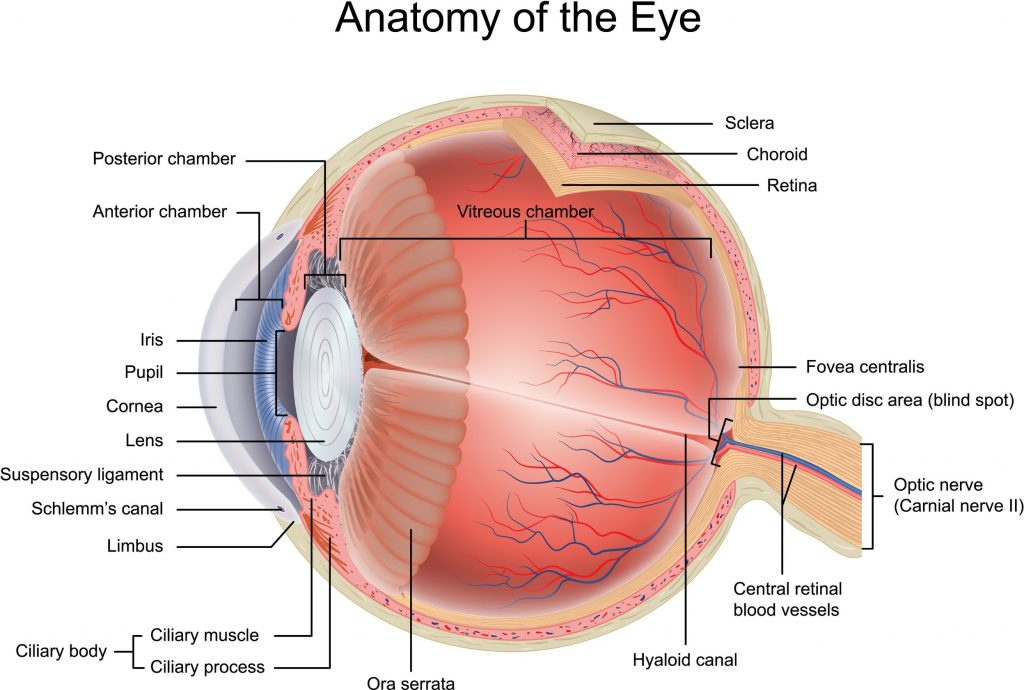
\includegraphics[width = 0.6
    \textwidth]{Images/Theory/occhio.jpg}
    \caption{Anatomy of the human eye.}
    \label{fig:ana}
\end{figure}

Despite its relatively small size, it contains an intricate arrangement of structures, each serving a distinct role in the process of vision.
At the very front lies the cornea, a transparent, curved surface that acts as the first point of contact for incoming light. 
Its main function is to bend, or refract, the light so that it can be properly directed toward the deeper structures of the eye.
Just behind the cornea is the iris, the colored part of the eye, which regulates the size of the pupil, the central black opening.[115] 
By widening or narrowing, the iris controls how much light enters the eye, functioning much like the aperture of a camera.
Positioned behind the iris is the lens, a flexible and transparent structure that fine-tunes focus. 
Through the action of tiny ciliary muscles, the lens can change its shape, allowing the eye to adjust focus when shifting between near and distant objects, a process known as accommodation.
Light then travels to the retina, a delicate layer of neural tissue lining the back of the eye. 
Far from being a passive screen, the retina actively processes the incoming light signals. 
It contains specialized photoreceptor cells, rods and cones, that convert light into electrical impulses. 
These signals are then transmitted through the optic nerve, a dense bundle of nerve fibers, to the brain's visual cortex, where they are interpreted and transformed into meaningful images.

\subsection{The retina and photoreceptor}

As we said earlier the retina plays a central role in vision, functioning as the site where light is transformed into neural signals that the brain can interpret. 
Within this thin layer of tissue reside two main types of photoreceptor cells, namely rods and cones, each of which is adapted for specific visual tasks.[115]

\begin{figure}[ht]
    \centering
    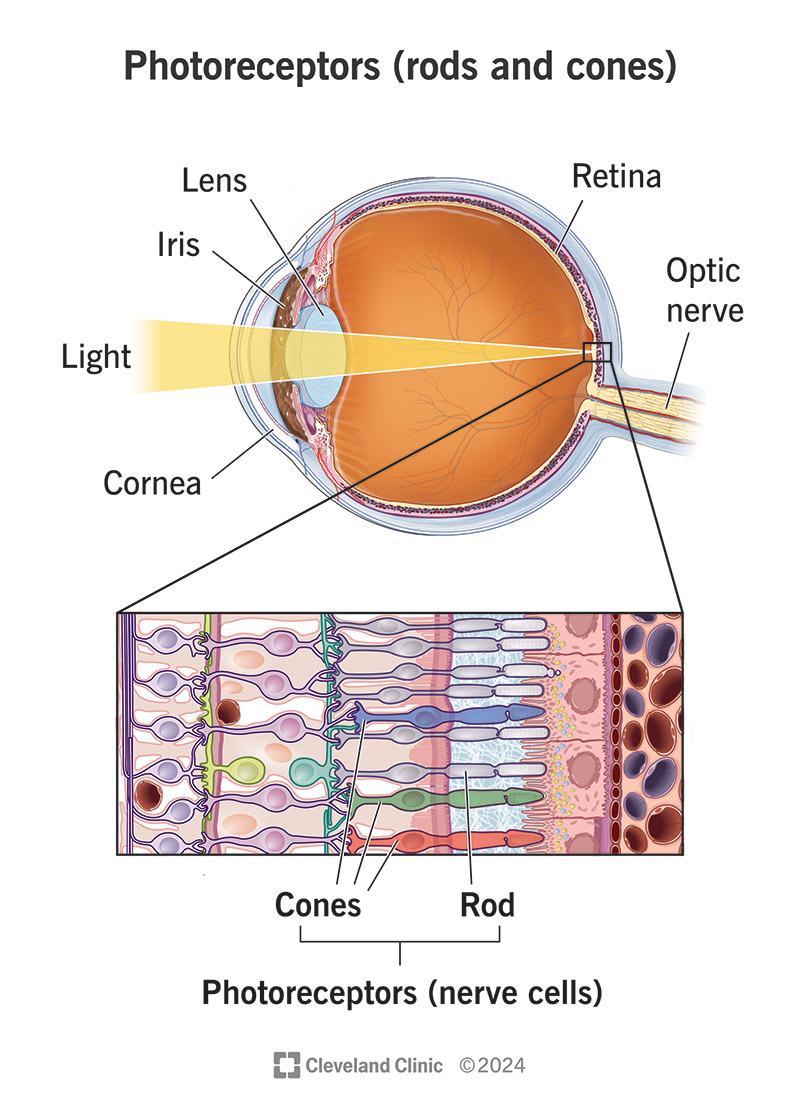
\includegraphics[width = 0.6
    \textwidth]{Images/Theory/rods_cones.jpg}
    \caption{Rods and Cones.}
    \label{fig:rodscones}
\end{figure}

Rods are highly sensitive to light and enable vision under low-light conditions. 
Although they do not mediate color perception, they are essential for detecting shapes, movement, and variations in brightness. 
Humans possess approximately 120 million rods in each eye, with the majority concentrated in the peripheral regions of the retina. 
This distribution explains why peripheral vision is far more effective in low-light environments, even though it lacks the ability to discriminate color.
Cones, by contrast, are less sensitive in low-light conditions but are indispensable for perceiving color and fine detail.
About 6 million cones are found in each eye, most of them concentrated in the central retina and especially within the fovea, a small depression that provides the sharpest visual acuity.
Cones are divided into three subtypes according to the wavelengths of light to which they are most responsive.
Some are sensitive to short wavelengths corresponding to blue light, others respond to medium wavelengths associated with green, and still others detect long wavelengths corresponding to red. 
The combined activity of these three types of cones forms the basis of human trichromatic vision, enabling us to perceive the full spectrum of visible colors.
This characteristic explains why the RGB color model is among the most widely used frameworks in digital imaging and display technologies.

\subsection{Color perception}

The process of color perception begins when incoming light stimulates the cones.
Each cone type has a broad response curve, meaning that their sensitivity ranges overlap. 
The brain does not simply interpret the activity of a single cone in isolation, but instead compares the relative responses of the three cone classes to determine the perceived color. 
For instance, strong activation of long-wavelength cones with weaker responses from the other two is interpreted as red. 
When medium- and long-wavelength cones are equally stimulated while short-wavelength cones contribute little, the result is perceived as yellow. 
If all three types respond at similar levels, the visual system interprets the signal as white. 
Thus, color vision is not a direct reading of individual wavelengths but an emergent property of neural comparison and integration across multiple cone pathways.
The interaction between rods and cones further illustrates the complexity of human vision.
Cones dominate during daylight conditions, but as light diminishes, rods become increasingly important.[115]
This shift, known as the Purkinje effect, reflects the higher sensitivity of rods to blue-green wavelengths.
As a result, red objects appear to darken as twilight falls, while blue ones remain more easily visible. 
Such changes highlight the complementary nature of rods and cones: one system optimized for detail and color in bright environments, and the other specialized for sensitivity in low-light conditions.

\subsection{Type of eye movements}

Human vision is not a static process. 
The eyes are in constant motion, guided by a sophisticated neuromuscular system that allows the fovea, the central region of the retina responsible for high acuity, to be directed toward relevant visual targets.
These movements are not random, but are precisely coordinated to stabilize images, explore the environment, and ensure that critical details are perceived accurately.
Almost all normal primate eye movements can be classified into five basic types: saccadic, smooth pursuit, vergence, vestibular, and physiological nystagmus.[21]
Each serves a distinct function, yet together they form an integrated system that balances accuracy, stability, and adaptability in visual perception.

Saccades are rapid, ballistic shifts of the eye that redirect the fovea from one point of interest to another.
They are the fastest of all eye movements, reaching velocities of up to 900 degrees per second, and typically last only a few tens of milliseconds. 
Despite their speed, saccades are precisely controlled, allowing humans to scan text when reading, explore complex scenes, or quickly detect changes in the environment. 
During saccades, visual sensitivity is temporarily reduced through saccadic suppression, preventing motion blur and maintaining visual stability.

In contrast to the abruptness of saccades, smooth pursuit movements allow the eyes to follow a moving object with remarkable fluidity. 
These movements are slower, generally limited to about 100 degrees per second, but are highly adaptive to the velocity of the target.
Smooth pursuit depends on both visual feedback and predictive mechanisms, as the eyes often anticipate the trajectory of an object to maintain accurate tracking.
This function is particularly critical for activities such as driving, sports, or any task where continuous monitoring of moving stimuli is required.

Vergence refers to the inward or outward rotation of the eyes that aligns them with targets at different depths.
Unlike saccades or pursuit, vergence movements are disjunctive: the two eyes move in opposite directions.
Convergence occurs when the eyes rotate inward to focus on a near object, while divergence refers to outward rotation for distant viewing. 
These adjustments are essential for depth perception and binocular vision, allowing humans to perceive the world in three dimensions.
Vergence movements are slower than saccades but are tightly linked with accommodation of the lens to maintain clear and unified images across distances.

The vestibular system, located in the inner ear, interacts with eye movements to ensure visual stability during head motion. 
The vestibulo-ocular reflex (VOR) automatically generates compensatory eye movements that counteract head displacement, allowing the gaze to remain fixed on a target even when the body is in motion.
For example, when walking or turning the head, the VOR maintains stable vision by producing equal and opposite eye rotations. 
This reflex is exceptionally fast, with response latencies of just a few milliseconds, underscoring its role in stabilizing vision in dynamic environments.

Although the eyes may appear still when fixating on an object, they are never completely motionless.
Physiological nystagmus refers to small, involuntary movements—including tremors, drifts, and microsaccades—that occur during fixation. 
These tiny displacements prevent the image on the retina from fading due to neural adaptation. 
Without them, stationary objects would gradually disappear from perception. Physiological nystagmus, therefore, is a crucial mechanism for maintaining continuous visual awareness of the environment, even when the gaze is held steady.

Though described separately, these five types of movements rarely operate in isolation. 
In natural vision, they combine seamlessly to provide both stability and flexibility.
For instance, during visual search, saccades bring the fovea to regions of interest, smooth pursuit maintains focus on moving targets, vergence adjusts for depth, vestibular reflexes stabilize the gaze against body motion, and physiological nystagmus ensures constant retinal stimulation.
Together, they form a dynamic and adaptive system that underpins the human ability to explore, interact with, and interpret the visual world.

\subsection{Fixation}

Fixation is the process by which the eyes maintain their gaze on a single point, allowing the visual system to capture and process detailed information from the environment.
Although the eyes may appear motionless during fixation, they are in fact never completely still.
Tiny involuntary movements such as microsaccades, tremors, and drifts occur constantly, preventing the image on the retina from fading due to neural adaptation and ensuring continuous visual awareness. 
These subtle motions are essential for maintaining clarity and precision, as they allow the fovea, the central region of the retina responsible for high-acuity vision, to remain accurately aligned with the target.
Fixation is fundamental to how humans interact with the visual world.
It provides a stable platform for extracting fine details, enabling activities that require careful attention, such as reading, inspecting objects, or monitoring a complex scene.
During fixation, the visual system is able to prioritize relevant information, enhancing perception and supporting higher-level cognitive processes such as attention, memory, and decision-making.
Even in dynamic environments, fixation works in concert with other eye movements: after rapid saccades redirect the fovea to a new location, fixation allows the visual system to stabilize and analyze the target.
While during smooth pursuit of moving objects, brief fixations may occur to refine the image and maintain accuracy.
Physiological nystagmus during fixation further ensures that retinal stimulation is continuous, allowing the perception of stationary objects to remain vivid and precise.
In essence, fixation is not merely a passive pause of the eyes but a dynamic and intricate process.
It balances stability and subtle motion, integrating seamlessly with other eye movements to support accurate, continuous, and detailed visual perception.
Without fixation, the human ability to explore, interpret, and respond to the environment with precision would be significantly impaired, highlighting its critical role in the visual system

\section{Eye tracking techniques}

After recognizing the importance of eye movements, it becomes clear that we need a tool to track them, and this tool is called an eye tracker.
In the past, eye trackers were highly expensive devices, mostly limited to research labs and specialized industries.
Over the years, however, their price has steadily decreased, making the technology more accessible.
Today, affordable solutions are available not only for scientific research but also for commercial applications such as gaming, marketing, user experience studies, and even healthcare.
This reduction in cost has opened the door to new innovations, allowing eye tracking to move from a niche tool to a widely adopted solution across many fields.
Eye trackers can be divided into two main categories: those that measure the position of the eye relative to the head and those that measure the orientation of the eye in space, also known as the Point of Regard (POR).
Building on this distinction, Chapter 5 of Eye Tracking Methodology: Theory and Practice [21] further identifies four methodological approaches to eye movement measurement: Electro-Oculography (EOG), scleral contact lens or search coil methods, Photo-Oculography (POG) or Video-Oculography (VOG), and video-based techniques combining pupil and corneal reflection.

\subsection{Electro-OculoGraphy (EOG)}

Electro-oculography (EOG) was the predominant method for recording eye movements around forty years ago and, although less common today, it still finds use in both clinical and research settings.
The technique operates by detecting differences in the corneo-retinal standing potential, which are measured through electrodes placed on the skin surrounding the eye. The recorded signal typically falls within the range of 15 to 200 µV, with a nominal sensitivity of approximately 20 µV per degree of eye movement. While EOG is effective for capturing eye movements relative to head position, it lacks the precision required for determining the point of regard. Consequently, its application for gaze tracking is limited unless combined with complementary systems capable of monitoring head movements, such as head trackers.

\subsection{Scleral Contact Lens/Search Coil}

One of the most accurate ways to measure eye movements uses a mechanical or optical reference attached to a contact lens that is worn directly on the eye. 
Early versions of this method, dating back to the late 19th century and later developed by Young and Sheena (1975) [22], used a plaster-of-Paris ring placed on the cornea, connected by mechanical linkages to recording devices.
Modern implementations use a scleral contact lens, which covers both the cornea and part of the sclera (the white of the eye) to prevent the lens from slipping.
A small mounting stalk is attached to the lens, and various devices can be placed on this stalk, such as reflective markers, line diagrams, or wire coils.
In magneto-optical eye-tracking systems, the wire coil is the most commonly used device. The coil is attached to the contact lens and moves together with the eye. 
As it rotates within a carefully controlled electromagnetic field, the system detects changes in the coil's orientation and generates precise measurements of eye movement. This setup allows extremely fine tracking of even very small rotations of the eye, making it one of the most accurate methods for recording eye position.
Based on Young and Sheena researches [22] the scleral search coil is extremely precise, with an accuracy of about 5–10 arc-seconds over a small range of roughly 5°. 
However, it is also highly invasive. 
Inserting the lens requires practice and care, and wearing it can be uncomfortable. 
In addition, this method measures the eye's position relative to the head, so it is generally not suitable for directly determining the point of regard.
\sloppy
\subsection{Photo-OculoGraphy (POG) or Video-OculoGraphy (VOG)}
\fussy
This category includes a wide range of eye movement recording techniques that rely on measuring distinct features of the eye during rotation or translation. 
Examples include the apparent shape of the pupil, the position of the limbus (the boundary between the iris and the sclera), and reflections from a nearby directed light source, often in the infrared spectrum. 
Although the specific methods differ, they are grouped together because they generally do not provide direct measurements of the point of regard. 
Measurements of ocular features in these techniques may be obtained either automatically or manually.
Manual visual inspection, such as reviewing recorded eye movements frame by frame on videotape, is extremely time-consuming, prone to error, and limited by the temporal sampling rate of the video device.
Automatic limbus tracking typically uses photodiodes mounted on spectacle frames and generally relies on invisible illumination, usually in the infrared range. Many of these methods also require the head to be held still, commonly using a head or chin rest, or a bite bar, to reduce movement (Young and Sheena, 1975)[22].

\subsection{Video-Based Combined Pupil/Corneal Reflection}

While the previously discussed techniques are generally suitable for measuring eye movements, they often do not directly provide point-of-regard measurements.
To determine the point of regard, either the head must be stabilized so that eye position relative to the head corresponds to gaze direction, or multiple ocular features must be tracked to distinguish between head movements and eye rotations.
Two key features commonly used for this purpose are the corneal reflection of an infrared light source and the center of the pupil.
Video-based eye trackers employ relatively inexpensive cameras and image-processing systems to calculate the point of regard in real time. 
These systems may be table-mounted or head-mounted.
The optical principles behind both configurations are essentially the same, with size and portability being the main differences.
Modern video-based eye trackers are compact and often integrated into monitors, making them particularly suitable for interactive applications.
In these systems, the corneal reflection, also known as a Purkinje image, is measured relative to the pupil center.
The human eye generates four distinct Purkinje reflections, which are formed by light reflecting off different surfaces within the eye: the anterior and posterior surfaces of the cornea, and the anterior and posterior surfaces of the lens (Crane, 1994) [23].
Each reflection carries unique optical information, but most video-based eye tracking systems rely primarily on the first Purkinje reflection, which is produced by the anterior corneal surface. 
This reflection is the brightest and most stable, making it well suited as a reference point for calculating gaze direction when measured relative to the pupil center.
With proper calibration, these trackers can reliably map a viewer's point of regard on a planar surface where calibration targets are displayed. 
Tracking both the pupil center and the corneal reflection allows the system to separate eye rotations from minor head movements.
Specifically, the relative position between the pupil and the first Purkinje reflection changes with eye rotation but remains nearly constant with small translations of the head.
More advanced systems, known as generation-V eye trackers, also measure the fourth Purkinje reflection (Crane \& Steele, 1985) [24].
These dual-Purkinje image (DPI) eye trackers can distinguish between translational and rotational eye movements: both reflections shift equally during translation, but they move differently during rotation, allowing the separation of the two effects.
Although highly accurate, DPI systems often still require the head to be stabilized for optimal performance. 
This is because even small head translations or rotations can introduce noise into the measurement, making it difficult to distinguish subtle eye movements from head motion. Stabilization methods, such as chin rests, bite bars, or other mechanical supports, are therefore commonly used to minimize artifacts.
While this limitation reduces the comfort and naturalness of the setup, it ensures the precision needed for research applications that demand extremely fine measurements of gaze direction.

\begin{figure}[ht]
    \centering
    % First row
    \begin{subfigure}[b]{0.45\textwidth}
        \centering
        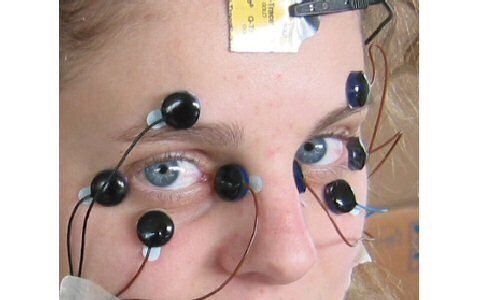
\includegraphics[width=1\textwidth,height=0.6\textwidth]{Images/Theory/eog.png}
        \caption{Electro-OculoGraphy (EOG) eye tracker.}
        \label{fig:eog}
    \end{subfigure}
    \hfill
    \begin{subfigure}[b]{0.45\textwidth}
        \centering
        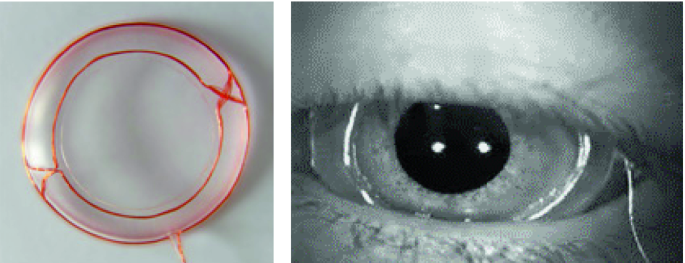
\includegraphics[width=1\textwidth,height=0.6\textwidth]{Images/Theory/coil.png}
        \caption{Scleral Contact Lens/Search Coil eye tracker.}
        \label{fig:coil}
    \end{subfigure}
    
    \vspace{0.5em}
    
    % Second row
    \begin{subfigure}[b]{0.45\textwidth}
        \centering
        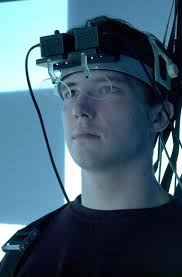
\includegraphics[width=0.7\textwidth,height=0.6\textwidth]{Images/Theory/vog.jpeg}
        \caption{Video-OculoGraphy (VOG) eye tracker.}
        \label{fig:vog}
    \end{subfigure}
    \hfill
    \begin{subfigure}[b]{0.45\textwidth}
        \centering
        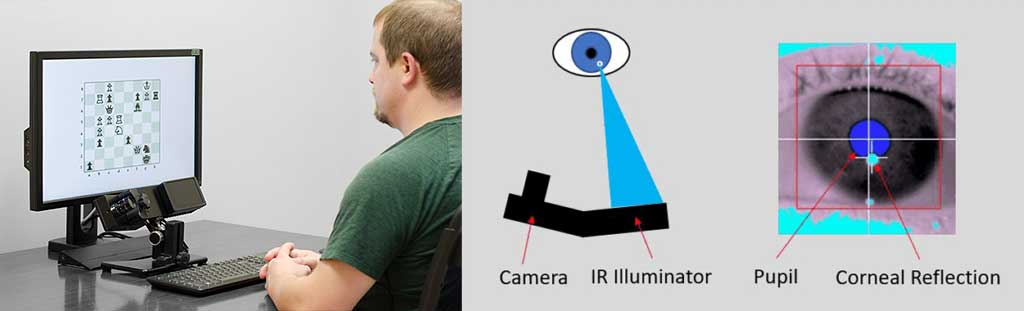
\includegraphics[width=1\textwidth,height=0.6\textwidth]{Images/Theory/corneal.jpg}
        \caption{Corneal Reflection eye tracker.}
        \label{fig:corneal}
    \end{subfigure}

    \caption{Different types of eye tracker.}
    \label{fig:four_grid}
\end{figure}

\newpage
\chapter{Related work}

This section presents an updated overview of the state of the art in gaze-based biometric solutions.
As a starting point, we draw on the work presented in Chapter 9 – Biometric Authentication to Access Controlled Areas Through Eye Tracking [25], published in 2017. 
Building upon this foundation, the review is expanded to include significant experimental studies and technological developments that have emerged in the years since, with particular attention to contributions up to 2025.
In this chapter, we deliberately exclude methods that rely on static characteristics of the human eye, such as iris-based recognition, which are already well established in biometric research. 
Instead, we focus on dynamic approaches, in which identity-related information is derived either from the manner in which an individual visually interacts with stimuli or from temporal changes in particular ocular characteristics.
The way an individual explores a visual scene, whether in a free-viewing context or under controlled conditions, can reveal distinctive patterns that serve as biometric cues.
In addition, time-dependent changes in ocular features, such as variations in pupil diameter, may provide further information useful for identity verification or recognition.
Building on this perspective, five principal categories of eye-tracking-based biometric techniques will be considered. 
The first includes ATM-like solutions, which simulate practical authentication scenarios.
The second focuses on fixation and scanpath analysis, where the sequence and duration of gaze points are examined. 
The third category emphasizes eye and gaze velocity, capturing the dynamics of eye movement. 
The fourth examines pupil size variations, which may be influenced by both physiological and cognitive factors.
Finally, the fifth category explores oculomotor characteristics and head orientation, integrating motor control features of the visual system into biometric assessment.

\section{ATM-like solutions}

This section begins with a review of gaze-driven authentication systems, which have been developed as alternatives to traditional password or PIN entry methods.
Such systems are particularly relevant in contexts resembling Automated Teller Machines (ATMs), where secure and efficient user authentication is essential. 
By replacing manual input on a keyboard with gaze-based interactions, these approaches aim not only to improve usability but also to reduce vulnerabilities such as shoulder surfing or keylogging, while at the same time opening new possibilities for integrating behavioral traits into the authentication process.
While these solutions are not strictly biometric, since the underlying information often comes from sequences of alphanumeric characters or graphical symbols, the way such sequences are entered through eye movements introduces behavioral elements that may carry biometric value.
For this reason, these approaches merit discussion as precursors to fully gaze-based biometric methods.

One of the earliest contributions in this area was presented by Maeder et al. [26], who explored gaze-directed authentication based on consciously fixating predefined regions of a visual stimulus for specified durations.
In their study, participants were shown an image of Prague divided into a non-uniform 3 × 3 grid.
Each user selected six “points of interest,” with one in each grid cell, and authentication was achieved by reproducing the same sequence of fixations.
In this design, the gaze path effectively served as a PIN, while the grid structure ensured both consistency and flexibility.

A further step toward practical implementations was proposed by Kumar et al. [27] in their system EyePassword, which aimed to reduce vulnerabilities such as shoulder surfing and eavesdropping. 
Four input modalities were compared: a traditional keyboard, gaze plus manual confirmation on an on-screen QWERTY keyboard, gaze with dwell time on a QWERTY layout, and gaze with dwell time on an alphabetic layout.
Although average entry times across the dwell and trigger-based methods were comparable (between 9.2 and 12.1 seconds), error rates were notably higher when a manual trigger was used (15\% versus 3–4\%).
These results highlighted both the feasibility of gaze input for secure authentication and the trade-offs between speed, accuracy, and usability.

In another line of research, De Luca et al. [28] proposed the use of eye gestures as authentication tokens. 
This method was inspired by the observation that visual patterns or geometric shapes are often easier to memorize than long alphanumeric strings. 
Here, authentication was performed by “drawing” gestures on the screen with the gaze, using eight basic directional strokes originating from or directed toward the screen's center. 
Such gestures represented an alternative form of input, combining memorability with the natural motor control of the eyes.

Similarly, Dunphy et al. [29] replaced numeric or textual credentials with a recognition-based scheme relying on faces. 
Users were asked to memorize a set of faces during an initial training phase and later authenticate by selecting them from sequences of grids containing distractor images. This approach emphasized recognition rather than recall, exploiting the human visual system's efficiency in face perception.

Other researchers explored the use of gaze interaction with symbolic keyboards. 
Weaver et al. [30] developed a system where authentication was achieved by looking at symbols arranged on a virtual keyboard.
Instead of relying solely on dwell time for character selection, gaze points were clustered and automatically analyzed to infer the intended input, thereby reducing delays and improving fluidity.

More recently, Cymek et al. [31] investigated authentication through smooth pursuit eye movements, which occur when the gaze follows a continuously moving target.
Their method used a moving PIN pad where each digit followed a unique trajectory, defined by a sequence of up, down, left, or right movements.
Authentication was achieved by tracking the trajectory of the correct digits with the eyes. 
Although this technique was slower than traditional dwell-time input, it offered distinct advantages: it reduced the need for calibration and made it more difficult for attackers to infer the entered PIN, since the input was encoded in movement patterns rather than in static gaze points.

Khamis et al. [37] conducted a rigorous comparison of cue-based authentication modalities for situated displays, focusing on touch, mid-air gestures, and calibration-free gaze. 
Through two in-depth user studies (N = 20, N = 17), they highlighted a clear tradeoff between usability and security. 
Gaze input was found to be more secure against shoulder-surfing attacks, but it was also more demanding and slower.
Mid-air gestures offered slightly higher security than touch, though they were less favored in public contexts.
Touch, on the other hand, remained the fastest but was less secure.
Their findings underline important design implications for balancing efficiency, security, and user acceptance in public authentication scenarios.

Omair Shahzad Bhatti et al. [36] proposed a calibration-free authentication method for interactive public displays based on saccadic eye movements, addressing the limitations of slower gaze-based approaches. 
In a user study with ten participants, their method was compared against CueAuth, a smooth pursuit-based system by Khamis et al. [37].
The results showed a substantial improvement in accuracy (82.94\% to 95.88\%) and a significant reduction in entry time (from 18.28s to 5.12s), making the approach comparable to touch-based input in speed while maintaining strong security.

Authentication systems are now widely used to protect personal information, but common approaches such as PINs, biometrics, and smart cards remain vulnerable. 
PINs are easily exposed through shoulder-surfing, biometrics can be spoofed, and smart cards are at risk of theft or duplication. 
To address these limitations, Ail Hamid Malla [38] proposes a gaze-based authentication system designed to counter shoulder-surfing, video-based observation, and spoofing attempts.
Experimental results demonstrate the effectiveness of the approach, achieving an accuracy of 97.5\% (F-measure = 0.97) in authenticating legitimate users and 89.5\% (F-measure = 0.89) in detecting intruder attempts.

Eye tracking has gained attention as a promising tool for biometric authentication, as eye movements are fast, distinctive, and require minimal effort from users.
However, earlier gaze-based systems often struggled with high error rates or slow authentication.
To address these issues, Ivo Sluganovic et al.[39] developed a method that uses reflexively triggered eye movements through interactive visual stimuli, enabling reliable feature extraction within seconds and eliminating the need for memorization. 
An additional advantage is that the stimulus can be uniquely generated for each login attempt, supporting a challenge–response mechanism that defends against replay attacks. 
A prototype tested with 30 participants demonstrated strong performance, achieving an equal error rate of 6.3\% and reducing authentication time to about 5 seconds, outperforming many prior approaches.

Matin Fallahi et al. [40] proposed a multimodal biometric authentication system for Extended Reality (XR), addressing the usability and security limitations of password-based methods. 
Traditional password entry in XR is cumbersome and error-prone, often leading to weaker password choices and reduced security. 
To overcome this, their approach combines eye movement patterns with brainwave signals, using consumer-grade sensors that can be seamlessly integrated into XR devices.
A prototype tested with 30 participants achieved an exceptionally low EER of 0.29\%, significantly outperforming single-modality systems based on eye movements (1.82\%) or brainwaves (4.92\%), as well as state-of-the-art biometric methods (EERs between 2.5\% and 7\%).
Importantly, this solution supports seamless and immersive authentication through visual stimuli, eliminating the need for complex user interactions.

Traditional authentication methods such as passwords overlook personal behavioral traits of users.
This study, suggested by Cantoni et al. [44], explores the use of eye-tracking data for biometric purposes during PIN entry via an on-screen virtual numeric keypad.
Both identification and verification are investigated. 
Machine learning algorithms are applied to analyze gaze patterns across the full PIN sequence as well as at the level of individual digits. 
The results, while not achieving the precision of traditional biometrics, are satisfactory within the context of soft biometrics, where the goal is to complement existing authentication methods—here, the PIN itself—by providing an additional layer of security.

Haochen Wang [47], in his thesis, presents four case studies evaluating gaze-based biometrics, including doorbell name inspection for building access, static image observation, moving target observation, and eye-driven soft PIN input.
Both identification and authentication were tested, including an analysis of user familiarity in the building access study. 
Results showed classification accuracies above 0.7 across most experiments, demonstrating the feasibility of gaze-based biometrics as a viable “soft biometric” method when combined with traditional authentication techniques.

\section{Methods based on fixation and scanpath analysis}

The use of fixations and scanpaths for biometric applications has been investigated for over a decade.
One of the earliest contributions was by Silver and Biggs [53], who compared keystroke dynamics with eye-tracking data for identification purposes. 
Although keystroke-based models clearly outperformed gaze-based ones, this work was among the first to highlight the potential of eye tracking as an alternative technique for biometric verification.

Subsequent studies have sought to extract and refine gaze features for improved performance. 
Holland and Komogortsev [54], for example, examined reading scanpaths using a high-frequency eye tracker (1000 Hz) and a dataset of 32 participants. 
They employed a wide range of features, such as fixation count, average fixation duration, and saccade amplitudes, as well as aggregate scanpath descriptors including path length, area, and inflection count.
By applying Gaussian cumulative distribution similarity measures and feature fusion, they achieved their best result with an EER of 27\%. 

In later work, Holland and Komogortsev [55] expanded this line of inquiry using both high-end (1000 Hz) and low-cost (75 Hz) eye trackers. 
From 32 and 173 participants, respectively, they extracted fixation and saccade features, which were analyzed with several statistical tests and machine learning classifiers. 
Their approach produced an EER of 16.5\% and a rank-1 identification rate of 82.6\%, demonstrating the potential of combining traditional statistics with machine learning for gaze-based biometrics.

Alternative methodologies have also been explored. 
Rigas et al. [56] introduced a graph-based approach in which fixations on face images were clustered using a minimum spanning tree (MST) technique.
Comparing overlap in MST structures between subjects enabled user identification with accuracies ranging from 67.5\% to 70.2\% across 15 participants and eight sessions.

Galdi et al. [57] conducted an experiment involving 88 participants across three sessions. 
Sixteen grayscale facial images were used as stimuli, and each image was divided into 17 Areas of Interest (AOIs) corresponding to facial regions (e.g., eyes, mouth, nose). 
For each participant, feature vectors were constructed by calculating the average fixation duration per AOI across all images. 
Using Euclidean and Cosine distance measures for comparison, the system achieved its best performance with combined features, reaching an EER of 0.361.

Cantoni et al. [33] extended this approach with a larger participant pool (111 from the first study plus 24 additional subjects one year later) and introduced the Gaze ANalysis Technique (GANT). 
Instead of manually defined AOIs, an automatic face normalization algorithm was applied to divide each image into a uniform 7×6 grid (42 cells).
Weights were calculated for each cell based on fixation density and duration, as well as for arcs connecting cells to capture gaze transitions. 
Similarity between models was assessed by comparing difference matrices via the Frobenius norm. Trials with both single and combined features showed that the best results were achieved when all features (density, fixation duration, and weighted paths) were fused, yielding a minimum EER of 28\%.

Further contributions expanded the scope of gaze-based biometrics beyond identity verification. Cantoni et al. [58] and Galdi et al. [59] applied features derived from GANT datasets to gender and age classification.
Using Adaboost and Support Vector Machines, they reported moderate success, with gender classification rates near 60\% and age classification rates around 55\%.

Other research has focused on task dynamics as a differentiating factor. Biedert et al. [60], for instance, examined task learning effects to detect unauthorized system access. 
They hypothesized that genuine users would navigate familiar interfaces fluidly, while impostors would exhibit higher exploratory behavior. 
To quantify this, they introduced the Relative Conditional Gaze Entropy (RCGE) method, which analyzes gaze distribution patterns.

George and Routray [61], winners of the BioEye 2015 competition, developed a highly effective approach to biometric identification. 
Using recordings from 153 participants across three sessions (two separated by 30 minutes and one by one year), they extracted extensive fixation and saccade features and applied backward feature selection with a Radial Basis Function Network (RBFN). 
Their method achieved success rates of 98\% across the shorter interval and 94\% across the one-year interval, highlighting the robustness of gaze-based biometrics under temporal variability.

Yin et al. (2022) [34] proposed a gaze-based authentication method leveraging the spatiotemporal features of eye movements.
To address the long recording times required by previous approaches, their method uses shorter eye movement recordings, recommending durations under 12 seconds based on deviations between gaze points and stimuli.
Temporal motion of gaze points and spatial saccade patterns were used to represent individual identity.
Experiments on two datasets (5 s and 12 s recordings) showed that open-set EER reached 10.62\% for 12 s and 12.48\% for 5 s, while closed-set EERs were 5.25\% and 7.82\%, respectively, demonstrating the method's effectiveness for rapid, eye-movement-based authentication.

The COVID-19 pandemic underscored the need for contactless authentication methods, particularly those based on eye or gaze features, which remain effective even when users wear masks and can complement traditional password or PIN systems. 
In this context, Porta et al. [35] presented a study on gaze-based soft biometrics that employed simple animations as visual stimuli, in which small squares moved along different patterns and trajectories without the need for preliminary calibration of the eye tracker. 
Machine learning analysis of the collected data demonstrated strong performance, especially in verification tasks, achieving accuracies above 80\% and EER often below 10\%.

The study, suggested by Yasmeen Abdrabou et al. [48], explores using gaze behaviour to assess perceived password strength, aiming to help users select passwords resistant to guessing attacks. 
We propose incorporating users' understanding of password strength into security mechanisms by analysing gaze patterns during password creation.
In a proof-of-concept study (N = 15), participants created both weak and strong passwords.
Results show that password strength can be predicted from gaze behaviour with 86\% accuracy using machine learning, paving the way for novel interfaces that encourage stronger password choices.

B. L. Tait [83] proposed a study in which 25 participants employed the EyeWriter eye-tracking system to assess whether individual eye movement behavior is sufficiently distinctive for secure biometric authentication.
The results indicate that behavioral eye movements can be effectively employed for biometric verification, particularly in a one-to-one authentication context, achieving success rates between 96\% and 100\%.
In contrast, one-to-many identification yielded an accuracy of only 21.83\%. 
While this demonstrates some potential, the limited sample size restricts the generalizability of the findings and highlights the need for further investigation with larger populations.

With the emergence of Virtual Reality (VR) displays equipped with embedded eye trackers, eye-tracking data is increasingly accessible and can be leveraged for applications such as gaze monitoring, privacy protection, and user authentication.
User identification is particularly critical in VR due to security and privacy concerns. 
Previous work has primarily relied on machine learning applied to motion-based data (e.g., body, head, eye, and hand tracking), typically requiring explicit tasks and extensive feature sets. 
In contrast, Asish SM et al. [84] proposed a system for user identification based on minimal eye-gaze features, without the need for identification-specific tasks. 
To evaluate user identification, gaze data from an educational VR application were processed with machine learning models (RF, kNN) and deep learning models (CNN, LSTM).
Results demonstrate that all models achieved identification accuracies exceeding 98\% using only six simple gaze features. 
The findings underscore the potential of eye-gaze–based identification in VR, while emphasizing its security and privacy implications and acknowledging the limitations of the current study.

\section{Methods based on eye/gaze velocity}

Bednarik et al. [62] investigated the potential of eye velocity as a distinguishing feature for biometric purposes.
They considered left-eye, right-eye, and combined velocity signals.
However, the results indicated very limited discriminative power, with identification rates ranging only between 6\% and 25\%.

Kinnunen et al. [63] proposed an approach based on the distribution of gaze angles over short temporal windows. 
The local velocity direction of the eyes was estimated using trigonometric transformations and represented in normalized histograms. 
Seventeen participants watched a 25-minute video while gaze data were collected at 120 Hz. 
Each participant was modeled using Gaussian Mixture Models, following a methodology reminiscent of speaker recognition. 
Depending on the amount of training and testing data available, error rates varied between 29.4\% and 47.1\%, reflecting moderate performance.

Rigas et al. [64] examined velocity and acceleration as biometric indicators by applying the Wald–Wolfowitz statistical test to compare distributions of dynamic eye features.
Their experimental design used a moving dot as stimulus, which jumped every 550 ms within grids of either 3×3 (Dataset A) or 2×2 (Dataset B) positions. 
Data were collected from 37 and 79 participants respectively, yielding 978 and 4168 signals. 
Fixations were extracted from these signals, and the classification results were encouraging, with identification rates of 96.6\% for Dataset A and 90.4\% for Dataset B.

Cuong et al. [65] introduced an alternative representation by encoding gaze features with Mel-Frequency Cepstral Coefficients (MFCCs). 
Features such as eye position, eye difference, and velocity were transformed into MFCC representations and classified using a single multi-class classifier, where the stimulus was represented by a moving point.
This approach emphasized the potential of signal-processing methods borrowed from speech recognition for eye-movement biometrics.

Liang et al. [66] explored acceleration-based features, focusing particularly on diagonal movements and one and two step shifts in both horizontal and vertical directions.
Five participants were instructed to repeatedly watch short video clips, and their eye movements were analyzed using both Back-Propagation neural networks and Support Vector Machine classifiers. 
The highest accuracy achieved in their work reached 82\%, suggesting that acceleration properties can provide stable biometric signatures even with relatively small sample sizes.

Darwish and Pasquier [67] concentrated on saccadic dynamics as a biometric source. 
Their study recruited 22 participants, with eye movements recorded at 120 Hz across four sessions scheduled twice weekly.
Stimuli included various patterns, such as a 4×4 dot matrix.
From the eye-movement data, several features were derived, including angular velocity and acceleration (for both left and right eyes) as well as absolute velocity. 
Mean, standard deviation, and maximum values of these metrics were then computed and used to train a Random Forest classifier with 10-fold cross-validation. 
This approach achieved strong results, with a Half Total Error Rate (HTER) of around 5\%.

Holland and Komogortsev [68] also incorporated velocity-based features into their framework.
Specifically, they extracted horizontal and vertical mean velocity along with peak velocities in both directions.
These parameters were used as part of a larger feature set to test classification models across datasets collected with both high-frequency and low-cost trackers.

Yoon et al. [69, 70] proposed a classification framework using velocity categories modeled through Hidden Markov Models (HMMs). 
In their first study [69], eye movements were captured from 12 participants with a 60 Hz eye tracker while they observed 250 still images composed of structured dot patterns (proximity grids, aligned grids, glass patterns, large shapes, and small shapes).
Velocity data were grouped into five states: extremely low velocity, fixation, smooth pursuit, saccade, and extremely high velocity. 
Using HMMs with five hidden states, classification accuracies ranged from 53\% to 76\%, with higher performance observed for participants with lower average gaze velocity. 
The second study [70] extended the analysis to 16 participants tested over morning and afternoon sessions. 
Here, HMMs were individualized by selecting the best likelihood across 2–5 hidden states per user.
While classification accuracies decreased to between 17\% and 41\%, the results confirmed that lower gaze velocity correlated with higher accuracy. 
They also noted better results for morning sessions, suggesting that fatigue might impair biometric consistency.

Juhola et al. [71] and Zhang et al. [72] focused on saccadic features for verification tasks. Juhola et al. compared data acquired from two eye trackers with very different sampling rates (400 Hz vs. 30 Hz) while participants followed a dot moving along a black bar.
They extracted amplitude, accuracy, latency, and maximum velocity of saccades and tested Linear Discriminant Analysis, Quadratic Discriminant Analysis, and Naive Bayes classifiers. 
High-frequency data led to recognition rates of around 90\%, whereas low-frequency recordings yielded 70–90\%. 
Zhang et al. extended this line of work by analyzing longer-term stability, with test intervals ranging from half a day to 16 months, using a 30 Hz tracker.
They added maximum acceleration and deceleration as features and employed classifiers such as Learning Vector Quantization, Discriminant Analysis, Naive Bayes, and Support Vector Machines. 
Verification experiments achieved up to 86\% accuracy for genuine users and 88\% for impostors with SVMs.

Srivastava et al. [73] combined velocity features with position and difference based features in an SVM multi-class classification framework. 
Using a moving point stimulus, their model consistently achieved high accuracy, exceeding 91\% across different test scenarios.

Eberz et al. [74] also incorporated temporal descriptors of saccadic dynamics into their biometric framework, focusing particularly on speed and acceleration.
These features were analyzed in conjunction with pupil size, thereby integrating both movement-based and physiological signals.
By combining dynamic saccade characteristics with pupillary responses, their study aimed to capture a richer representation of user-specific visual behavior. 
This multimodal approach demonstrated that temporal aspects of saccades, when fused with pupil-based metrics, can enhance the distinctiveness of biometric profiles and contribute to more reliable user identification.

Ali, Hoque, and Deravi [45] proposed a presentation attack detection method based on directed gaze trajectories, where randomized visual stimuli are used to trigger natural pupillary motion, making spoofing attempts harder to succeed. 
Their system was tested with photo, 2D mask, and 3D mask artifacts on data collected from 80 volunteers.
The results demonstrated that gaze trajectory features are effective in distinguishing genuine users from presentation attacks, confirming the potential of this approach for enhancing biometric security in practical applications.

Spoofing is a major challenge for biometric systems, and a gaze-based method using randomized visual stimuli has been proposed to detect such attacks.
Ali et al. [46] propose a method based on the idea that natural head–eye coordination during gaze shifts creates unique accuracy patterns that are difficult for impostors to mimic.
Data collected from genuine users and from attackers employing photographs, 2D masks, or replayed videos were analyzed using features derived from collinear and colocated gaze points. 
Experimental results, including both isolated feature evaluations and score-fusion combinations, demonstrated the effectiveness of the method in distinguishing between authentic and spoofed attempts.

Harezlak K et al. [49] evaluated biometric identification using eye movement signals by testing new features, including frequency-domain representations and the largest Lyapunov exponent, alongside velocities and accelerations.
Eye movement data were recorded in 100-ms segments from 24 participants across two sessions, as they observed a point appearing at 29 screen locations. 
Feature vectors were created for single points and sequences of three points. 
Two training/testing scenarios were tested: one with 75\% of randomly selected vectors and equal participant representation, and another using separate sessions for training and testing.
Decision tree and random forest classifiers performed best, with random forest achieving up to 100\% accuracy in the first scenario, while performance dropped significantly in the second.

\section{Methods based on pupil size}

Despite receiving relatively limited attention as a biometric trait, pupil size has emerged as a promising indicator for both identification and verification, as evidenced by several noteworthy investigations.

Bednarik et al. [62], previously discussed in relation to other ocular features, also examined the role of pupil size in biometric recognition. 
Their experimental setup included 12 participants exposed to four types of visual stimuli: text, a static cross, a moving cross, and an image.
The features extracted comprised pupil size (left, right, and combined), delta pupil size (for left, right, and combined), eye velocity (left, right, and combined), and interocular distance.
In addition, aggregate mean values of these attributes were examined, and the analysis employed Fast Fourier Transform (FFT), Principal Component Analysis (PCA), as well as their combined application.
Performance was assessed using both individual features and weighted feature fusion. 
The best single-feature result was achieved with eye distance, yielding a 90\% success rate.
However, as this measure relates more closely to physical rather than behavioral characteristics, its biometric validity is limited.
Among behavior-related features, delta pupil size achieved the strongest outcome (60\%). When feature fusion was applied, combining eye distance with other features consistently resulted in accuracies exceeding 90\%.

Nugrahaningsih and Porta [75] extended this line of inquiry by evaluating pupil size as a soft biometric in a longitudinal setting. 
Their study involved 25 participants tested across two sessions separated by one year. 
The experimental task was minimal, requiring subjects only to fixate on a plus sign displayed at the center of a white background.
Key attributes included left and right pupil sizes, along with their ratio and difference.
Each attribute was described by 15 statistical measures (e.g., minimum, maximum, mean, variance, median, geometric mean, harmonic mean, interquartile range, kurtosis, skewness, and range). 
Additional features included the sum of squared differences and the correlation between left and right pupil sizes.
Classification was performed using four algorithms: Naïve Bayes, Neural Networks, Support Vector Machines (SVM), and Random Forests.
Results indicated higher identification performance when selected subsets of features were employed (0.6194–0.7187), while verification performance remained consistently strong across both full and reduced feature sets ( $\approx$0.97).

Eberz et al. [76] further explored the discriminative power of pupil size by incorporating it into a larger framework of 21 features.
Pupil-based measures included maximum, minimum, mean, standard deviation, and range of pupil diameter. 
Participants were instructed to click as quickly as possible on red dots with white centers that appeared sequentially in random screen locations.
Three experimental conditions were used: no prior instruction, textual guidance, and a visual preview of the dot locations. 
In addition to pupil features, temporal and spatial eye-movement features were also considered. 
Classification was performed using k-Nearest Neighbors (kNN) and Support Vector Machines. 
Across the three experimental settings, EER ranged from 3.98\% to 9.27\%, underscoring the value of combining pupil size with dynamic ocular features for reliable biometric identification.

The following work, proposed by Casanova et al. [51], develops a web user identification model by analyzing behavioral biometrics from touch dynamics and periocular characteristics such as pupil movements, blinks, and fixations.
A feature-level fusion approach is applied, combining different distance measures (Euclidean, Bray-Curtis, Manhattan, Canberra, Chebyshev, Cosine) to determine whether a test sample matches the target subject.
Multi-data processing methods such as Canonical Correlation Analysis (CCA) and Principal Component Analysis (PCA) are used to further enhance performance.
Results show that fusing these biometric traits significantly improves accuracy, achieving over 92\%, surpassing individual biometrics.

\section{Methods based on oculomotor features}

Kasprowski and Ober [77] investigated the use of Cepstral analysis, the inverse Fourier transform of the logarithm of a signal's power spectrum, as a biometric feature.
Eye movement data were collected with a 250 Hz tracker from nine participants instructed to follow a 3×3 jumping point stimulus, with each participant enrolled on 30 occasions. 
The dataset consisted of “probes” representing eye movement recordings during eight-second stimulations. 
From these data, 15 cepstral coefficients were extracted across four waveforms and subsequently used as input to four classifiers: K-Nearest Neighbors (KNN), Naïve Bayes, Decision Tree, and Support Vector Machine (SVM). 
Classification performance was assessed using 10-fold cross-validation, yielding an average False Accept Rate (FAR) of 1.48\% and a False Reject Rate (FRR) ranging between 6.7\% and 43.3\%, with an overall average of 22.59\%.

Building on different physiological properties, Komogortsev et al. [78] examined oculomotor plant characteristics (OPC) as a verification biometric. 
Their method extracted saccadic parameters from eye-tracking data and transformed them into nine OPC components using a linear homeomorphic 2D oculomotor plant model. 
These components included length tension, series elasticity, passive viscosity, agonist and antagonist force–velocity relationships, tension intercept, agonist and antagonist tension slopes, and eye globe inertia. 
Two statistical techniques—Student's t-test with Voting and Hotelling's T² test—were employed to measure similarity between OPC vectors, with an additional AND/OR fusion strategy to combine classifier outcomes. 
Using a 1000 Hz eye tracker, data were collected from 59 participants across two sessions separated by a 20-minute break, during which participants followed a jumping dot stimulus. 
The best result achieved was a minimum Half Total Error Rate (HTER) of 19 \%, using both Hotelling's T² test and the OR Student's t-test with Voting for horizontal saccadic data.

In a subsequent contribution, Komogortsev et al. [79] explored a multimodal ocular biometric framework by integrating three distinct traits: OPC, Complex Eye Movement (CEM) patterns, and the physical structure of the iris.
While iris recognition is not the primary focus of this survey, it was included in their study alongside OPC and CEM features, both derived from eye movement dynamics captured via image sequences. 
A Sony PlayStation Eye camera was employed to record both iris and eye movement data, using Rorschach inkblot images as stimuli.
Data from 87 participants were analyzed, and results demonstrated that combining these ocular traits improved overall accuracy and enhanced the resistance of the system against spoofing attempts.

Liang et al. [80] complemented their use of acceleration-based features by integrating muscle properties into the framework, with particular attention to seven “optimum muscle parameters.”
These parameters were derived to capture the biomechanical characteristics of the oculomotor system, reflecting how individual differences in muscular control influence eye movement dynamics.
By integrating these physiological descriptors into their biometric model, the authors demonstrated that muscle-based features can provide complementary information to traditional kinematic measures, thereby enhancing the distinctiveness and reliability of gaze-driven biometric identification.

Dillon Lohr et al. [42] investigated the fusion of two eye-centric authentication modalities—eye movements and periocular images—within a calibration-free framework. 
While both modalities have demonstrated promise individually, their integration in a unified pipeline had not been studied extensively at scale.
Using a large in-house dataset of 9,202 subjects with eye-tracking quality comparable to consumer-grade VR devices, the authors showed that their multimodal approach consistently outperformed unimodal systems and surpassed the FIDO benchmark.
The use of advanced machine learning models enabled the system to capture complementary discriminative features from both modalities, significantly enhancing authentication performance.

In 2023 Alessandro D'Amelio et al. [43] proposed a principled framework for modeling eye movements as a form of behavioral biometrics, drawing on foraging theory as a basis for capturing the uniqueness of individual gaze behavior. 
A composite Ornstein–Uhlenbeck process is employed to characterize the exploration–exploitation dynamics of eye movements, with parameters inferred from eye-tracking data through Bayesian analysis.
These parameters serve as discriminative features for biometric identification, which is performed using standard classification techniques.
A proof of concept on a publicly available dataset demonstrates the effectiveness of the approach, highlighting its potential both for biometric applications and for advancing the analysis of eye-tracking data.

The increasing need for secure digital access, coupled with technological advances and the lack of standardized solutions, continues to drive research into eye movement–based biometrics.
This work, suggested by Harezlak and Plucienni[81], presents two neural network–based approaches to user identification from eye movement dynamics.
In the first method, a 100-element time series was constructed to represent eye movement features, including velocity, acceleration, jerk, point-to-point percentage changes, and frequency-domain characteristics. 
These were modeled using a Long Short-Term Memory (LSTM) network. 
The second method employed the same dynamic features but derived statistical descriptors from the time series, which were then classified using a dense neural network.
Experiments were conducted with the publicly available GazeBase dataset, focusing on recordings obtained under the “jumping point” stimulus condition. 
Results demonstrate strong discriminative potential: the LSTM model with time series feature vectors achieved 96\% accuracy, while the statistical feature–based method achieved 76\%. 
These outcomes were observed across a three-year span of recordings, with analyses also considering different temporal segments and stimulus configurations.

The work suggested by Abbas Seha et al. [85] examines the biometric potential of eye movement patterns from low frame rate eye-tracking devices.
It also explores recognition improvements through additional static and dynamic ocular features, such as eye blinking patterns and periocular shape characteristics.These modalities are relevant for applications like continuous driver authentication in law enforcement. 
Two datasets were collected using different low frame rate eye trackers, recording eye movements from 55 participants during real driving sessions. 
For eye gaze, fixation and saccade features—including duration, amplitude, and statistical descriptors—were extracted.
Blinking features included patterns, speed, acceleration, and power-per-unit-mass profiles, while periocular features comprised eye-opening height, width, and axial ratio. 
Each modality was evaluated individually, then combined in a multi-modal fusion. While single modalities showed moderate performance, fusion of static and dynamic features significantly improved results, achieving up to a 98.5\% recognition rate and 0\% error rate. 
This demonstrates that, although single-modality approaches may lack robustness, multi-modal fusion offers high reliability for continuous driver authentication.

\section{Methods based on head orientation}

Cazzato et al. [32] introduced an alternative to traditional eye trackers by employing the depth and RGB streams of the Microsoft Kinect sensor.
Their approach did not aim to precisely determine the exact gaze point.
Instead, it relied on cases where head orientation could be treated as a reasonable approximation of gaze direction, followed by a rough estimation of pupil position.
Because gaze could not be assessed in every video frame due to computational delays and occasional failures in detecting the face or pupil, the missing values were estimated using Kalman Filter predictions. 
The gaze detection process consisted of two stages. In the first stage, head pose was estimated using the depth and RGB data. 
In the second stage, pupil position was determined from the RGB stream. 
These two components were then combined to calculate the final X and Y gaze coordinates. 
Feature extraction was carried out using Principal Component Analysis (PCA), and the selected features were classified through a Minimax classifier.
Experiments were conducted with 12 participants who watched three short video clips. 
The results showed that precision ranged from 81\% to 83\%, while recall ranged from 80\% to 86\%.

M. Wierzbowski et al. [50] conducted an investigation involving 43 participants who viewed multiple 360-degree VR videos while their eye-tracking data and headset orientation were recorded.
Using both deep learning and classical statistical methods, the researchers tested whether a viewer of a previously unseen VR video could be identified based on prior viewing data. 
The experiments achieved a maximum average identification accuracy of 75\%, demonstrating the potential for identifying VR users under unforced behavioral conditions.

This research, conducted by Rubo et al. [52], investigates the feasibility of implicit user identification in Social Virtual Reality (VR) based solely on eye gaze patterns during dyadic interactions.
Employing Siamese Convolutional Neural Networks on data from 128 participants, the study achieved an identification accuracy of 95.50\% by combining models for gaze during speaking and listening. 
Findings indicate that gaze patterns constitute distinctive, idiosyncratic behavioral traits, largely independent of self-reported personal characteristics.
These results underscore significant privacy and security implications for Social VR environments, where gaze data may be collected passively under conditions of limited movement and variable data quality.

Identifying users of a Virtual Reality (VR) headset enables adaptive interface design, personalization of settings, and adjustment of difficulty levels in both gaming and training applications.
While most existing identification methods require explicit input, implicit user identification offers a less intrusive alternative that preserves immersion.
Liebers et al. [82] proposed a biometric identification system leveraging gaze patterns and head orientation during stimulus tracking for user recognition.
The method was validated through a user study, with a hybrid post-hoc analysis yielding identification accuracies of up to 75\% using an interpretable machine learning model and up to 100\% with a deep learning approach.
Finally, potential application scenarios are discussed, demonstrating how this approach can enable seamless and implicit user identification in VR environments.

Recent research has explored identifying users in virtual reality (VR) based on behavioral data. 
These approaches often rely on elaborate authentication tasks resistant to “shoulder surfing” but overlook whether identification is possible under natural behavior.
In the study by Wierzbowski et al. [86], involving 43 participants, the authors investigated whether a viewer of an unseen 360° VR video could be identified using eye-tracking and headset orientation data recorded while viewing other 360° VR videos.
Using deep learning and classical statistical methods, we achieved up to 75\% average identification accuracy, demonstrating the potential for VR user identification under unforced conditions.
\newpage

\chapter{Experiments}

Considering the advantages offered by behavioral biometric approaches, this research aims to investigate their effectiveness in the context of a novel application.
In particular the thesis will focus on a specific field of research in this discipline called Gaze-based biometric.
Gaze-based biometrics is a field that investigates the behaviour of a user who reacts to a visual stimulus.
In this study, we propose to record subjects gaze patterns using an eye-tracking device, capturing a range of descriptive features.
The analysis will focus on identifying the specific points of visual attention and extracting meaningful information from these gaze behaviors.
This approach not only allows for a detailed characterization of individual visual patterns but also facilitates the development of models to evaluate their performance in both identification and verification tasks.
There are two types of stimuli that can be used for Gaze-based biometrics: Static stimuli or dynamic stimuli.
A static stimulus refers to an object displayed on the screen that remains fixed, such as a still image, whereas a dynamic stimulus involves an animation that changes its properties or behavior over time.
In this work, we employed a dynamic stimulus consisting of moving text that changes its position over time.
The stimulus was designed with two speed conditions (slow and fast) and two font sizes (small and large), resulting in a total of eight distinct stimuli.
We selected dynamic text as our stimulus because this area remains largely unexplored in the context of gaze-based biometrics.
In contrast, previous studies proposed by Holland et al. [54] and Bednarik et al. [62], have primarily focused on static text stimuli for biometric applications.
The objective of this research is to apply machine learning techniques to evaluate the performance, for identification and verification, of these kinds of stimuli and determine the most effective animation. 
Although these prior studies have examined static text, we also conducted a preliminary experiment with static text to enable a direct comparison under the same experimental conditions.

\section{Set up}
At the beginning, before starting the analysis, a phase was performed to collect the data and create the dataset.
The data collection involved 35 participants, including 22 males and 13 females, the majority of whom were university students.
Of the participants, 17 were aged 25 or younger, 13 were between 26 and 40 years old, and 4 were over 40. 
Additionally, 18 wore eyeglasses, while only one wore contact lenses.

\begin{table}[ht]
    \centering
    \caption{Participants’ data.} % caption appears above
    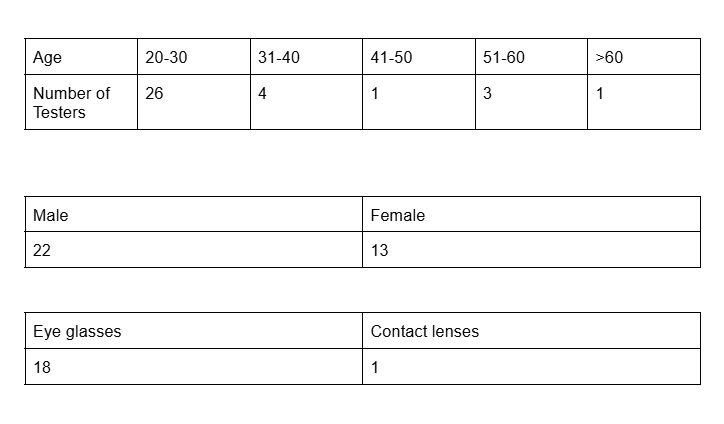
\includegraphics[width=0.6\textwidth]{Images/Experiment/tester.png}
    \label{tab:test}
\end{table}


A detailed overview is provided in Table \ref{tab:test}.

All recordings were carried out under identical artificial lighting conditions, with the same light source activated for each session.
The experiments took place in a quiet environment, free from noise and distractions, using an eye tracker mounted on a monitor to record participants' gaze. 
No additional information regarding the task was provided to the participants aside from the instruction to read and follow the text, even when it moved fast. 
Furthermore, no participant was exposed to any of the texts or animations prior to their first trial, ensuring unbiased and spontaneous responses throughout the experiment.

The participant was seated on a height-adjustable chair and asked to observe the stimuli presented on the monitor. 
The monitor, a 23-inch display with a resolution of 1920×1080 pixels (full-HD), was positioned in front of a white wall and equipped with an eye tracker. 
Research carried out in controlled laboratory settings with high-frequency eye trackers, often requiring the use of a chin rest, has demonstrated that very high recognition rates can be achieved [89].
However, such conditions are not realistic for practical applications, as high-frequency devices are costly and the use of a chin rest is inconvenient for everyday scenarios. 
In real-world contexts, lower-frequency eye trackers should be employed without physically constraining the user's head. 
For this reason the eye tracker used was a GazePoint GP3\_HD, configured with a data sampling rate of 150 Hz, and employed in our experiments without head restraints.
We also chose to conduct the recordings without calibration. 
While calibration is typically a short procedure, lasting between 15 and 30 seconds, it inevitably lengthens the overall authentication process and can become inconvenient or even frustrating for users. 
More importantly, although calibration is generally straightforward in controlled laboratory conditions, it is far less reliable in real-world contexts. 
Users may fail to remain perfectly still, or external factors such as background noise and the presence of other people can easily disrupt the process, rendering the calibration ineffective [35].
This decision, however, restricted the use of gaze coordinates as features in the analysis, due to the lower accuracy compared to a calibrated setup.
Nevertheless, we consider this approach to be more practical and representative of real-world conditions, where performing calibration is often impractical and unsuitable for continuous or everyday authentication scenarios.

With regard to the experimental procedure, each participant completed nine trials, organized into three separate sessions (S1, S2, and S3).
Each session was conducted on a different day, with the second and third sessions occurring no more than a month after the preceding ones. 
Consequently, the total testing period for each participant ranged from a minimum of 3 days to a maximum of 30 days, with an average duration of 10 days.
During each session, participants completed the test three times, referred to as “trials” (T1, T2, and T3), with a one-minute break between trials. 
Before each session, participants were simply instructed to read the text displayed on the screen without receiving any explanation of the experiment's purpose.
The participant was positioned approximately 50–60 cm from the monitor, with a possible additional adjustment of up to 15 cm to ensure a comfortable viewing angle for the eye tracker.

\begin{figure}[htbp]
    \centering
    \begin{subfigure}[t]{0.45\textwidth}
        \centering
        \includegraphics[height=5cm, angle=0]{Images/Theory/eye-tracker.png}
        \caption{GP3\_HD Eye-Tracker device.}
        \label{fig:et}
    \end{subfigure}
    \hfill
    \begin{subfigure}[t]{0.45\textwidth}
        \centering
        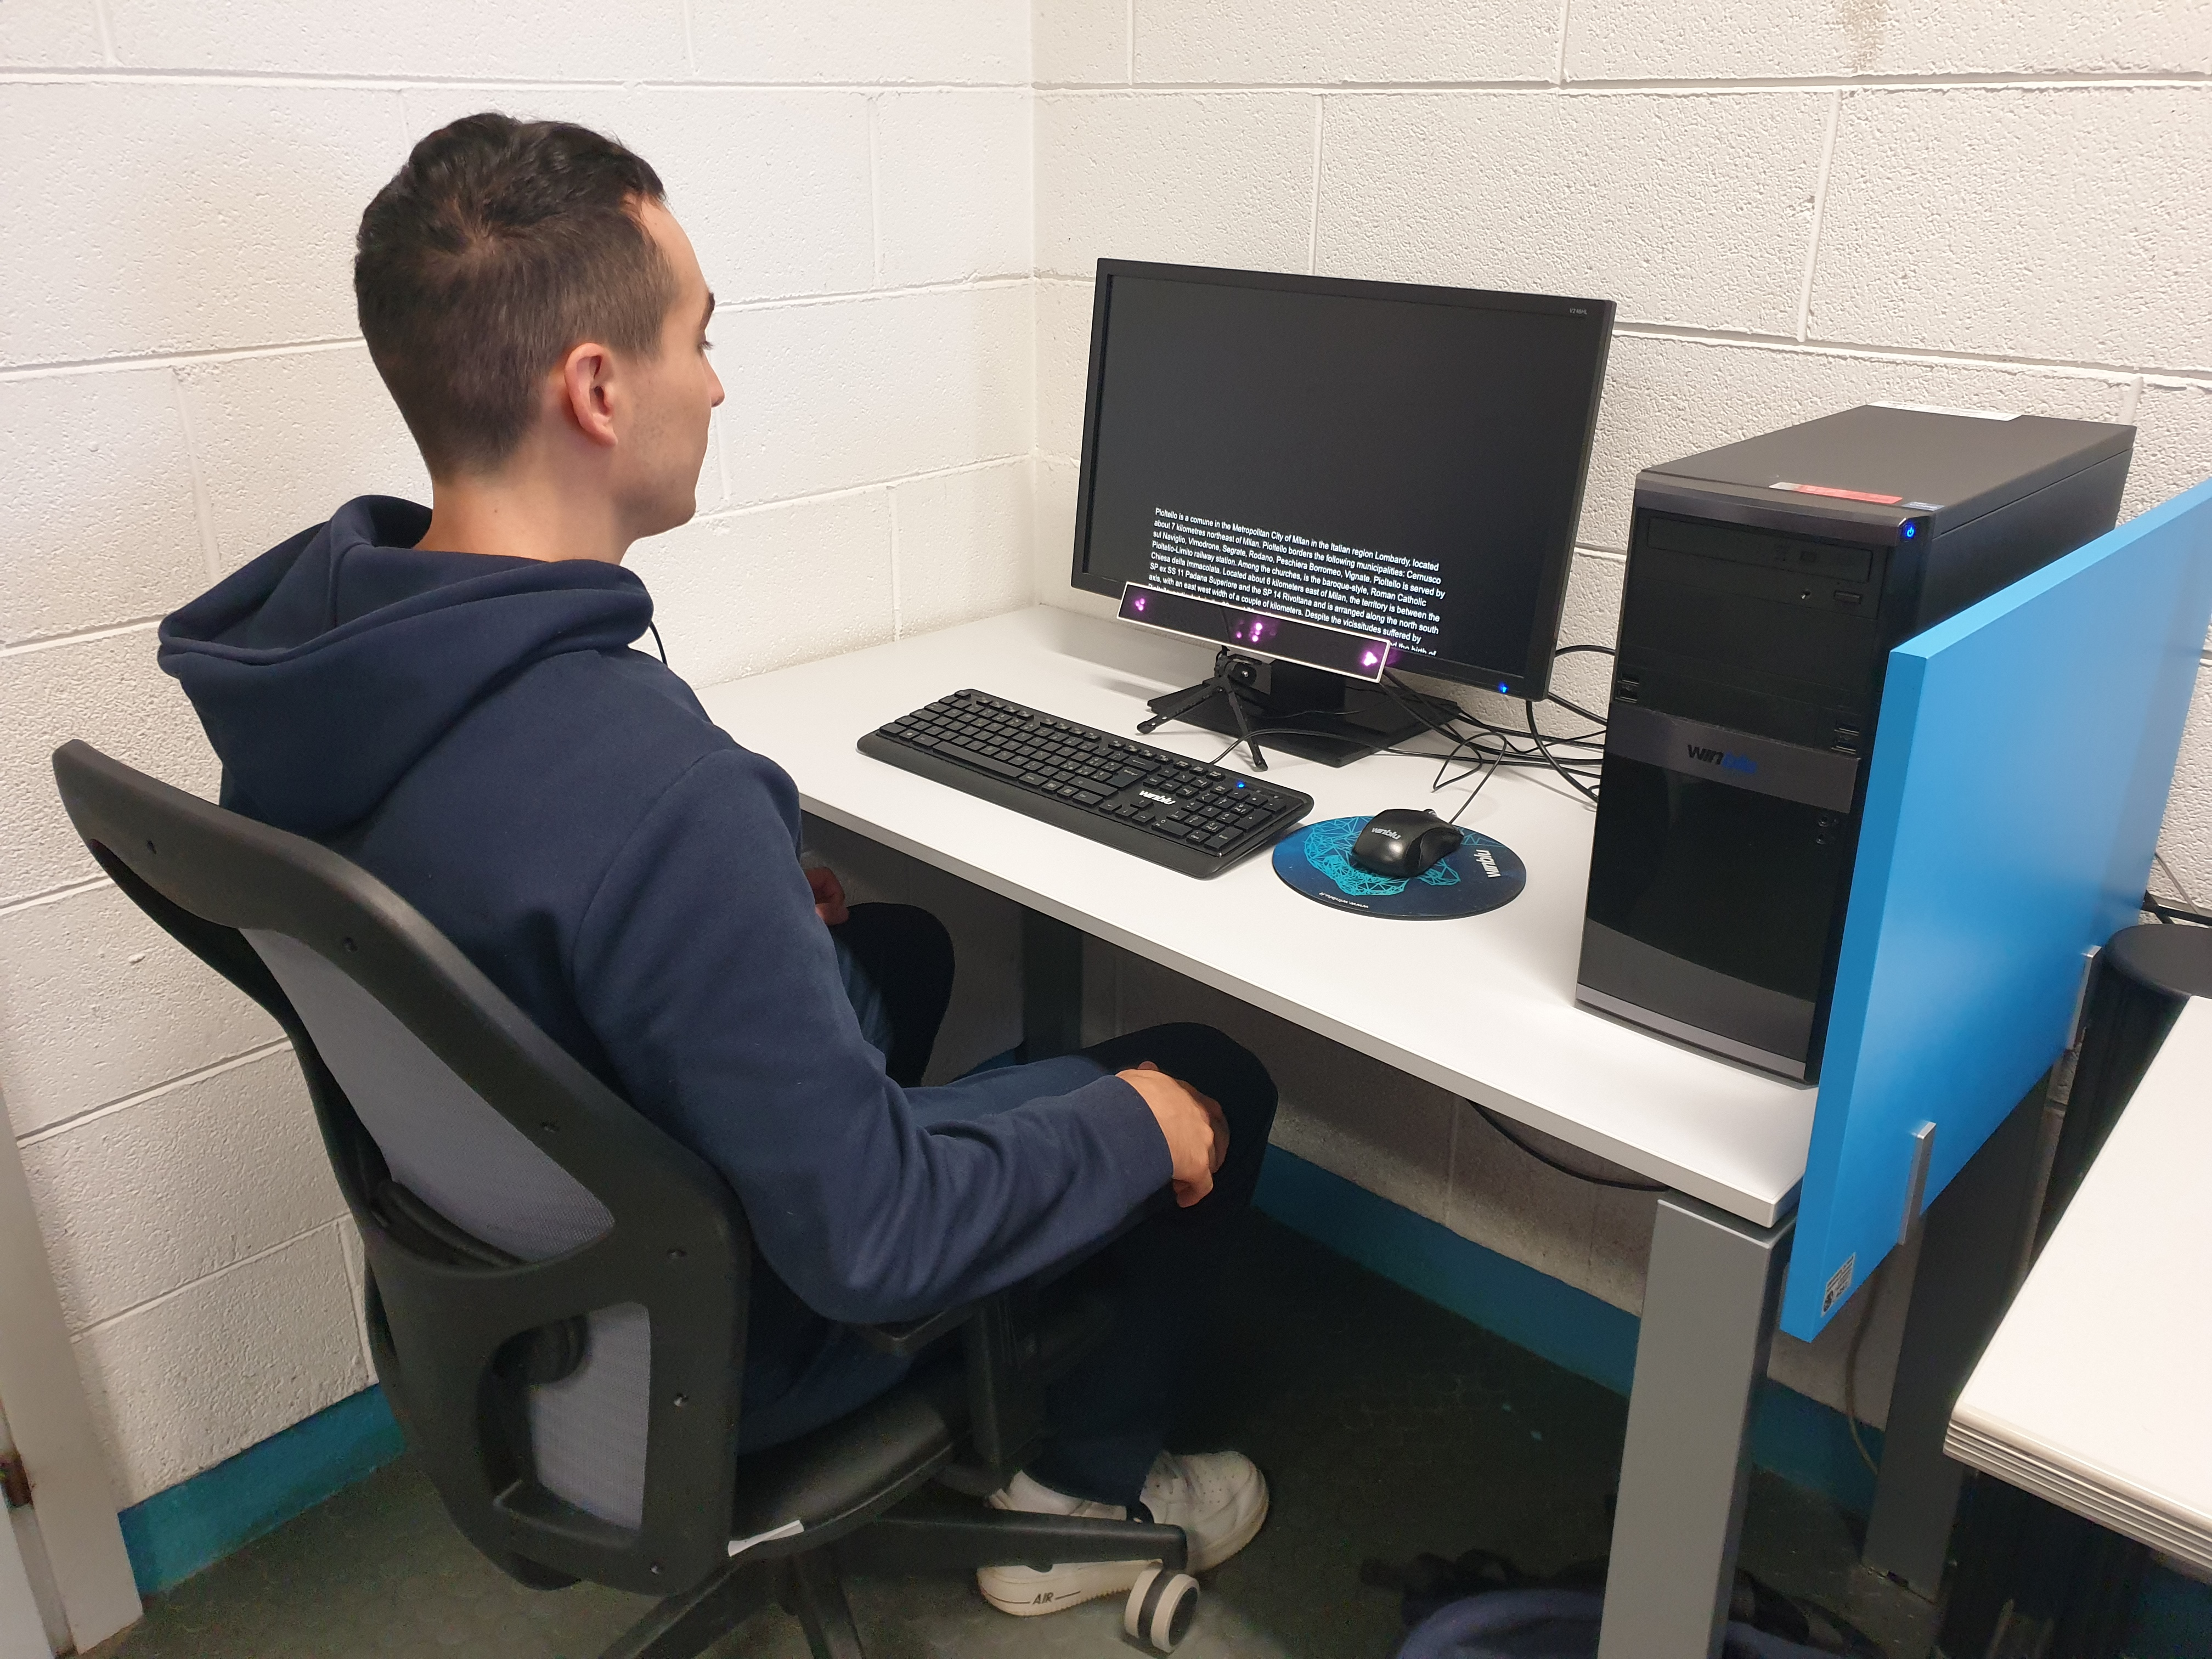
\includegraphics[height=5cm]{Images/Theory/sample.jpg} 
        \caption{Subject attending to the stimuli during data collection.}
        \label{fig:sample}
    \end{subfigure}
    \label{fig:et_sample}
\end{figure}


\FloatBarrier

\section{Stimuli}
\label{subsec:stimuli}

Since the field of gaze-based biometrics using dynamic text is largely unexplored, it was challenging to determine which types of stimuli would be most suitable to select.
The initial idea was to use a white rectangular block containing black text, displayed on a black background, which moved by bouncing off the screen borders until the animation time expired.
At that stage, only four animations were implemented, each differing in the initial position of the block and the direction of its movement.

However, these animations were unusual for text and we preferred to adhere to a classic format and employ a type of text that is most frequently encountered in everyday contexts. 
Consequently, we selected two types of animations for the study: Horizontal Scroll and Vertical Scroll.
The Horizontal Scroll animation consists of a single line of text presented continuously. 
The text initially appears at the middle right of the screen and moves steadily toward the left. 
As the animation progresses, additional characters are gradually revealed, producing a continuous scrolling effect. 
This presentation is analogous to the running text commonly utilized in television news broadcasts, thereby providing a familiar stimulus for gaze-based biometric analysis.
The Vertical Block animation consists of a block of text occupying approximately two-thirds of the screen width. 
The block moves steadily from the bottom toward the top of the screen in a continuous manner, similarly to the credit roll seen at the conclusion of films. 
This animation offers a different motion pattern for gaze behavior analysis and serves as a complementary stimulus to the Horizontal Scroll animation, enabling a comparative evaluation of gaze dynamics in distinct movement contexts.

The previously mentioned animation types were further diversified to generate a total of eight distinct stimuli for the experiment. 
Specifically, each animation type was implemented with two different font sizes (large and small) and two movement speeds (slow and fast), resulting in eight unique animation conditions to be tested.

\subsection{Preliminary experiments}

Preliminary experiments were carried out aimed at selecting appropriate text speed and size parameters. 
To address this question, we conducted a brief exploratory study in the laboratory involving seven participants.

\begin{table}[ht]
    \centering
    \caption{Participants' data.} % caption appears above
    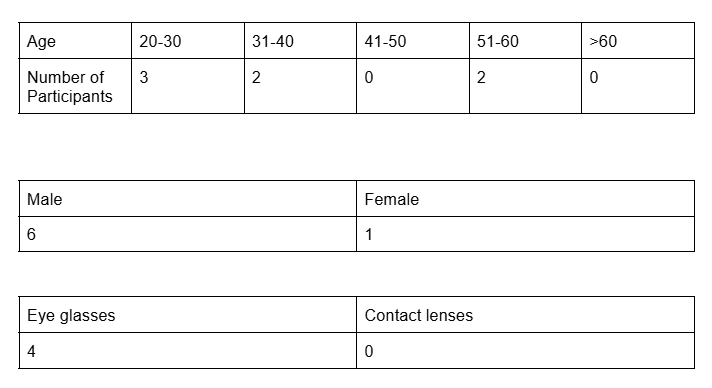
\includegraphics[width=0.6\textwidth]{Images/Experiment/tester_speeds.png}
    \label{tab:prel}
\end{table}

The demographic data of these participants are presented in Table \ref{tab:prel}. 
The group consisted of six males and one female and four participants wore eyeglasses. 
Regarding age distribution, three were between 21 and 30 years old, two between 31 and 40 years old, and two between 51 and 60 years old.

The first experiment was aimed at determining the minimum font size at which text remains comfortably readable on the screen during the movement. 
Different-sized text was displayed and participants were asked to select the smallest font size at which they felt confident in reading it. 
In addition to the animated stimuli, a static text was presented to participants to allow them to indicate their preferred font size. 
Rather than relying on specialized software, we manually selected a range of font sizes and displayed the animations to illustrate how each size would appear.
We then solicited opinions from laboratory members to determine the minimum legible size, and based on this collective input, agreed upon the most suitable values.
From these suggestions, we identified the largest value among the minimum sizes chosen, which was adopted as the baseline for the experiment. 
It should be noted that the selected font size may have been influenced by the age of certain participants, as variations in visual acuity and reading comfort can affect preferences. 
Although this size may appear relatively large, it was considered appropriate for the animation format, ensuring clarity and ease of reading under dynamic viewing conditions. 
This decision prioritizes both readability and consistency across participants, which is essential for the reliability of gaze-based biometric analysis. 
Consequently, the font size for the “small text” condition was set to 30 pixels, while the “large text” condition was defined as twice this size, at 60 pixels.

The objective of the second experiment was to determine the maximum speed at which a participant can still read our dynamic text. 
For the purposes of this research, it was not essential for participants to read the entire text. 
Rather, it was sufficient that they could perceive and process at least a portion of it. 
This approach reflects the nature of gaze-based biometric authentication, where the goal is to verify an individual's identity based on eye movement patterns rather than a full comprehension of the displayed content. 
In practical applications, authentication can be successfully achieved without requiring the user to fully understand or read every element of the stimulus, as the biometric signature lies in the gaze behavior itself rather than in the complete reading of the text.
Participants were instructed to select the highest speed at which they were still able to follow the text and comprehend it.
Specifically, for the horizontal scroll animation, they were asked to read as much as possible, while for the vertical block animation, they were required to read at least the firsts lines of the text.
For this purpose we developed a custom software application in Python to present both types of animations, namely horizontal scroll and vertical block, using the previously selected font sizes.
This resulted in a total of four animation conditions: horizontal scroll with small font (HS-small), horizontal scroll with large font (HS-large), vertical block with small font (VB-small), and vertical block with large font (VB-large).
During the experiment, participants were instructed to read the text and progressively increase its speed by pressing a keyboard key. 
They continued this process until the speed ation became too high to follow the text.
In this experiment, we deliberately set aside the requirement for participants to read the text comfortably, as our primary interest was not in reading comprehension but in determining the maximum speed at which the text could still be followed.
At that point, participants could either revert to the previous speed if the current one was too fast, or confirm the current speed as their preferred maximum readable speed by pressing a key.
This procedure allowed us to determine a personalized speed threshold for each animation condition, reflecting the highest speed at which participants could still read and track the text. 

Rather than assigning the same speed to both horizontal and vertical text scroll, we determined a distinct speed for each. 
This choice was motivated by the fact that the perceptual effort required to follow a moving text depends not only on the kind of movement (horizontal scroll vs. vertical block) and font size. 
For example, a speed that is comfortable for a large-font vertical block may become unreadable when applied to a small-font horizontal scroll.

\begin{table}[ht]
    \centering
    \caption{Speeds data per animation.} % table-style caption
    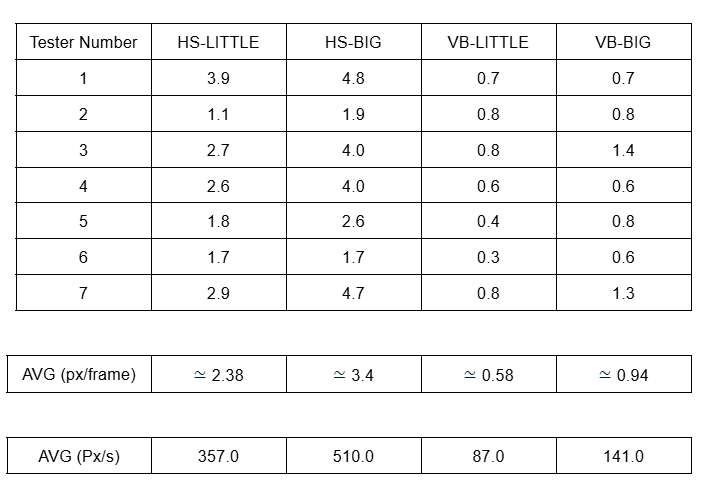
\includegraphics[width=0.6\textwidth]{Images/Experiment/speeds.png}
    \label{tab:sped}
\end{table}


In our implementation, the scrolling speed of the text stimulus is defined as the number of pixels by which its position is updated at each frame of the animation.
A frame represents a single iteration of the display update cycle in a computer-based animation or graphical application. 
In this study, the visual stimuli were implemented using Pygame, a Python library for creating interactive graphics.
In Pygame, each frame corresponds to one complete execution of the main loop, during which the visual scene is refreshed on the screen. 
Consequently, the frame rate, typically measured in frames per second (FPS), determines how many times per second the display is updated and, therefore, how smoothly motion or animation appears.
This means that speed is expressed in terms of pixels per frame inside our program. 
At first sight, the use of non-integer values for speed may seem counterintuitive, since pixels are discrete entities on the display and cannot be physically subdivided. 
The adoption of floating-point values, however, is a standard practice in computer graphics. 
While the rendering process ultimately positions the stimulus at integer pixel coordinates, the internal position of the object is stored as a floating-point variable. 
This allows the accumulation of fractional displacements across successive frames, such that sub-pixel movements are realized over time. 
Without this approach, the animation would appear jerky or imprecise at low speeds, as small displacements would be lost due to rounding. 
In this way, the use of decimal values for speed ensures the perceptual continuity of motion, despite the discreteness of the display grid.

It is important to note that the measure of speed in pixels per frame is directly dependent on the refresh rate of the display. 
In the present setup, the frame rate is explicitly fixed at 150 frames per second. 
This choice is not arbitrary, but rather motivated by the need to synchronize the visual stimulus with the eye-tracking device, which samples gaze data at the same frequency of 150 Hz. 
Such temporal alignment ensures that each frame of the animation corresponds precisely to one sample of eye-tracking data, thereby facilitating a consistent and interpretable mapping between stimulus motion and recorded gaze behavior.

To convert the per-frame displacement into a more conventional measure of velocity, namely pixels per second, it is sufficient to multiply the displacement per frame by the number of frames per second. 
Following this procedure, a speed of 2.38 pixels per frame corresponds to 357 pixels per second, while values of 3.4, 0.58, and 0.94 pixels per frame translate to 510, 87, and 141 pixels per second, respectively. 
These values provide an interpretable indication of the actual velocity of the stimulus as perceived on the screen.
All these values are summarized in Table \ref{tab:sped}, which first presents the speeds chosen by each participant for each animation, and then reports the average of these speeds expressed both in pixels per frame and in pixels per second.

From the perspective of the participant, these velocities determine the apparent rate at which the text traverses the display from right to left. 
Higher values, such as 357 or 510 pixels per second, result in a rapid motion where the text crosses the screen in a relatively short amount of time, demanding faster eye movements to track it. 
In contrast, lower values such as 87 or 141 pixels per second correspond to a slower drift of the text, allowing for more prolonged fixations and smoother pursuit. 
Thus, expressing the stimulus velocity in terms of pixels per second not only provides a standardized physical measure of speed but also offers a direct connection to the perceptual experience of the task and to the temporal dynamics of oculomotor responses.

Although in the present study the frame rate was fixed at 150 Hz to match the sampling rate of the eye tracker, the same principle applies to different refresh rates. 
If the animation were instead run at 60 Hz or 120 Hz, the conversion from pixels per frame to pixels per second would need to be recalculated accordingly, leading to proportionally different velocities for the same per-frame displacement. 
This illustrates that the absolute value of stimulus speed cannot be interpreted independently of the frame rate, and highlights the importance of reporting both parameters in experimental contexts.

In conclusion we decided to adopt the mean speeds computed for each type of animation, averaged across the data collected from the seven participants, as the reference values for the “fast” condition of the experiment.
This approach allowed us to derive a standardized measure of fast speed that reflects the natural preferences of the participants while ensuring consistency across stimulus types. 
For the “slow” condition, we chose to set the speed at exactly half of the corresponding fast speed for each animation. 
This decision was motivated by the desire to create a clear and perceptually meaningful distinction between the two conditions, while maintaining proportional scaling across animations. 
Subsequently, we implemented these values in the experimental program and performed a qualitative verification of the resulting motion. 
The observed scrolling speeds were found to be perceptually acceptable and consistent with the intended experimental design, providing confidence that the chosen parameters would yield reliable and interpretable results in subsequent testing.

\subsection{Animations}

In the previous sub-section, we conducted a preliminary study to define the parameters of the experimental setup—specifically, the text speed and character size—ensuring that these values were selected based on empirical evidence rather than chosen arbitrarily. 
This preparatory step was essential to establish a solid methodological foundation for the subsequent experiments. 
Having established the parameters, we can now present and describe in detail the eight animations used as stimuli in our gaze-based biometric research. 
These were systematically constructed by combining the two animation types (Horizontal Scroll and Vertical Block) with two font sizes (small and big) and two movement speeds (slow and fast). 
This design yielded eight distinct conditions, providing a comprehensive basis for evaluating the effectiveness of dynamic text as a biometric modality.

The animations are detailed below:

\begin{itemize}
    \item \textbf{VB\_SL\_SMA}: Vertical Block animation with \emph{slow speed} and \emph{small text size}. 
    In this condition, the block of text scrolls upward from the bottom to the top of the screen at the low speed, with characters displayed at the minimum legible size identified during the preliminary study.
    The parameters correspond to a font size of 30 pixels and a scrolling speed of 0.29 px/frame.

    \item \textbf{VB\_SL\_BIG}: Vertical Block animation with \emph{slow speed} and \emph{large text size}. 
    Similar to VB\_SL\_SMA, but the increased character size facilitates readability, while maintaining the slower scrolling speed. 
    In this case, the configuration employs a font size of 60 pixels with a speed of 0.47 px/frame. 

    \item \textbf{VB\_FA\_SMA}: Vertical Block animation with \emph{fast speed} and \emph{small text size}. 
    In this case, the upward scrolling occurs at the maximum speed identified in the preliminary study, with the minimum character size, representing a challenging condition for the user.  
    The setting combines a font size of 30 pixels with a speed of 0.58 px/frame.

    \item \textbf{VB\_FA\_BIG}: Vertical Block animation with \emph{fast speed} and \emph{large text size}. 
    The rapid upward motion is combined with larger text, allowing participants to more easily perceive and follow the characters despite the increased pace.  
    This version uses a font size of 60 pixels together with a scrolling rate of 0.94 px/frame. 

    \item \textbf{HS\_SL\_SMA}: Horizontal Scroll animation with \emph{slow speed} and \emph{small text size}. 
    The text enters from the right edge of the screen and scrolls steadily toward the left at the slower rate, with characters displayed at the smaller size.  
    The parameters here are a font size of 30 pixels and a speed of 1.19 px/frame. 

    \item \textbf{HS\_SL\_BIG}: Horizontal Scroll animation with \emph{slow speed} and \emph{large text size}. 
    This condition presents the same horizontal scrolling movement, but with larger text, facilitating readability at the slower pace. 
    The chosen configuration corresponds to a font size of 60 pixels and a scrolling speed of 1.7 px/frame. 

    \item \textbf{HS\_FA\_SMA}: Horizontal Scroll animation with \emph{fast speed} and \emph{small text size}. 
    The text moves quickly from right to left, with small character dimensions, providing the most visually demanding condition in terms of both speed and size. 
    In this setup, the font size is 30 pixels and the speed reaches 2.38 px/frame. 

    \item \textbf{HS\_FA\_BIG}: Horizontal Scroll animation with \emph{fast speed} and \emph{large text size}. 
    In this case, the high-speed scrolling is mitigated by the increased character dimensions, offering a balance between perceptual clarity and dynamic movement.  
    The applied parameters are a font size of 60 pixels combined with a scrolling speed of 3.4 px/frame.
\end{itemize}

An important aspect to consider in the design of the experiment concerns the textual material used in the animations. 
Since the primary objective of this research is to investigate gaze-based biometrics, it was crucial to ensure that the chosen text did not introduce biases related to content interest or familiarity. 
If certain passages were perceived as more engaging, informative, or familiar than others, this could have inadvertently affected participants' reading behavior and consequently distorted the study. 
To minimize this risk, we opted for neutral and homogeneous material by selecting descriptive texts taken from Wikipedia entries of municipalities in Lombardy, Italy.

A total of 72 unique texts were employed, corresponding to the experimental design (8 animations × 3 trials × 3 sessions). 
This ensured that each stimulus presentation featured a distinct text, thereby minimizing the risk of repetition effects or memorization influencing the results.
To further enhance methodological rigor, texts were randomly selected for each trial, ensuring that each participant was exposed to a unique sequence of stimuli. 
This approach prevented systematic biases and increased the generalizability of the findings by diversifying the conditions across participants.
Similarly, the order of animation presentation was randomized for every trial, mitigating potential sequence effects such as learning, fatigue, or adaptation.
To manage these randomizations and guarantee appropriate stimulus distribution, the experimental software integrated an SQL database to track previously displayed texts. 
This system automatically assigned unused texts for each trial, ensuring that all participants experienced varied and unbiased stimuli. 
By combining randomized text selection with randomized animation order, the design maintained both experimental consistency and stimulus neutrality across sessions and participants.

Prior to the presentation of each animation within a trial, a fixation stimulus consisting of a white cross displayed on a black background was shown(Figure \ref{fig:cross}).
This cross was positioned at the center of the screen to act as a visual anchor, directing participants' gaze to a consistent starting point before the animation began. 
The inclusion of this fixation stimulus serves two important purposes. 
First, it standardizes the initial gaze position across trials and participants, which reduces variability that could affect gaze tracking accuracy. 
Second, it ensures that participants are focused and visually prepared for the upcoming stimulus.
This procedure enhances the reliability of the data by controlling for differences in initial eye position, which is especially critical in gaze-based biometric research where precise tracking of eye movement patterns is essential.

In conclusion each trial comprised eight animations, each with a duration of 15 seconds. 
Before each animation, a fixation cross was presented for 2 seconds at the center of the screen to (implicitly) guide the participant's gaze and establish a consistent starting point. 
The total duration for a single trial was therefore (8 × 15) + (8 × 2) = 136 seconds per trial.
During the same day, each tester completed three trials, each lasting 136 seconds, for a total of 136×3=408 seconds, or approximately 6 minutes and 48 seconds. 
To complete the three sessions, the tester engaged in 136 × 3 × 3 = 1,224 seconds, which corresponds to a total of 20 minutes and 24 seconds of experimental exposure.

\begin{figure}[ht]
    \centering
    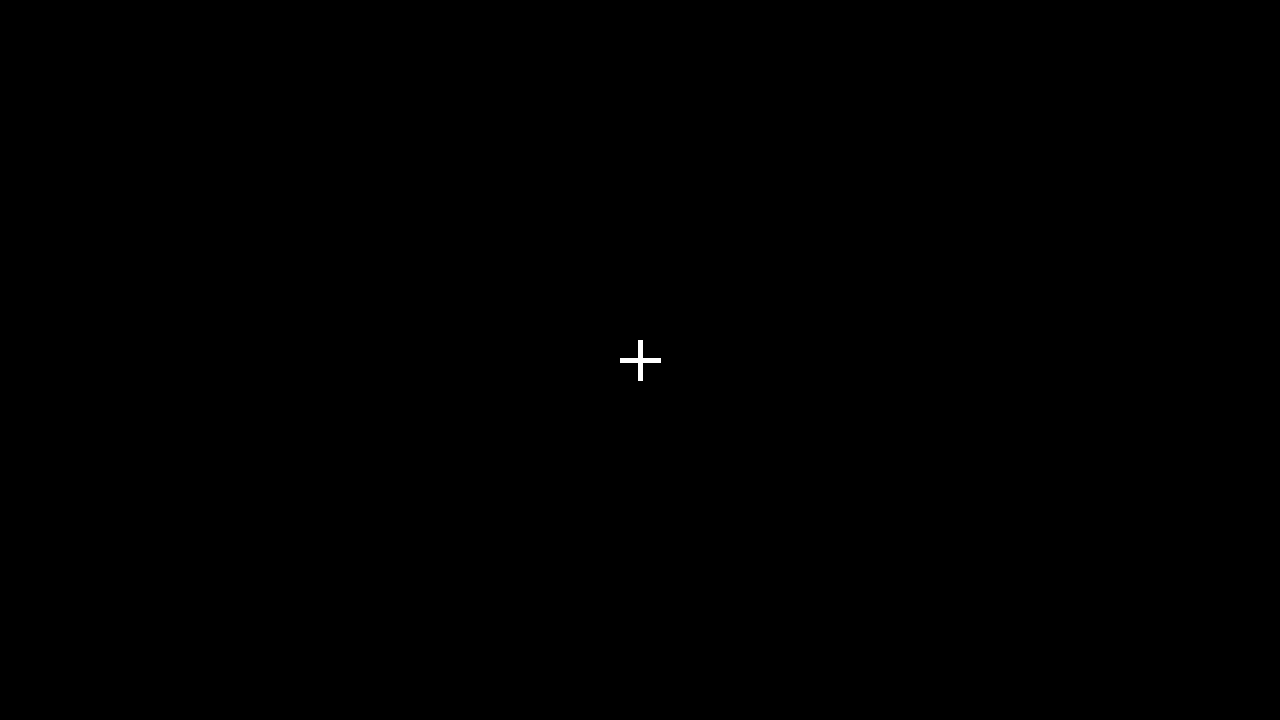
\includegraphics[width = 0.6
    \textwidth]{Images/Experiment/cross.png}
    \caption{White cross animation.}
    \label{fig:cross}
\end{figure}

\begin{figure}[ht]
    \centering
    % First row
    \begin{subfigure}[b]{0.45\textwidth}
        \centering
        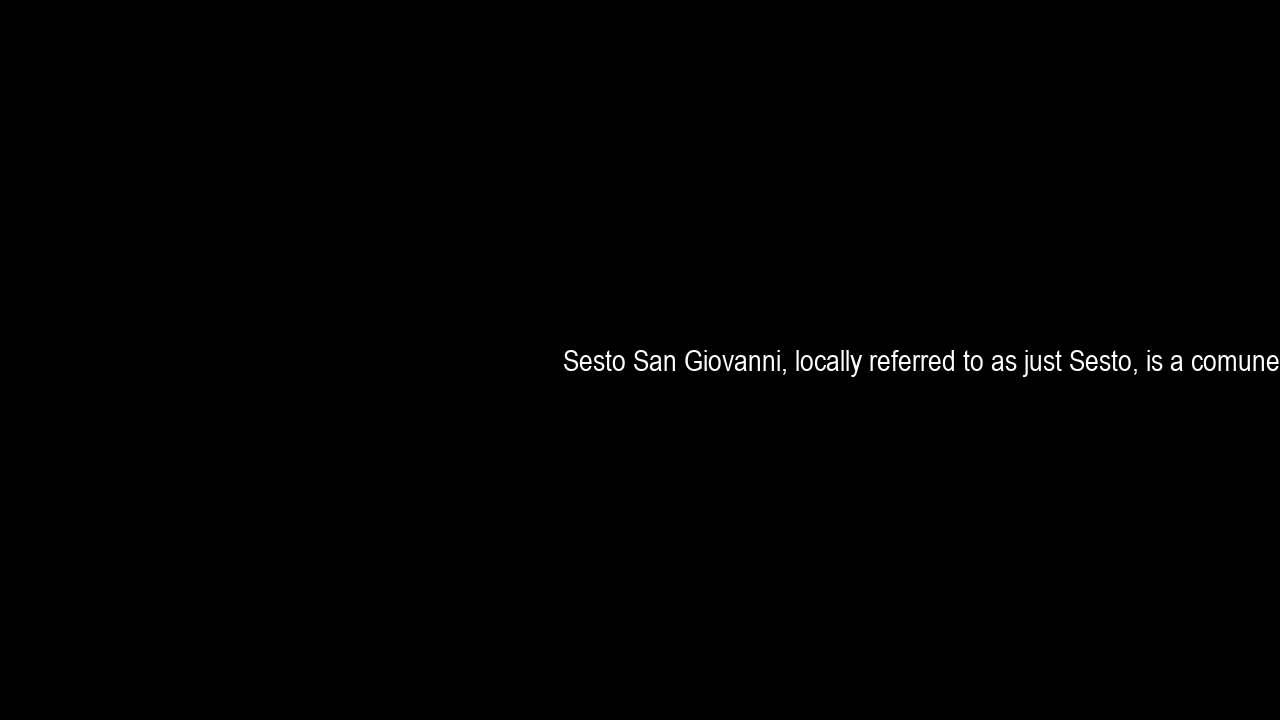
\includegraphics[width=1\textwidth,height=0.6\textwidth]{Images/Experiment/HS_little.png}
        \caption{Horizontal scroll, small text.}
        \label{fig:HS_L}
    \end{subfigure}
    \hfill
    \begin{subfigure}[b]{0.45\textwidth}
        \centering
        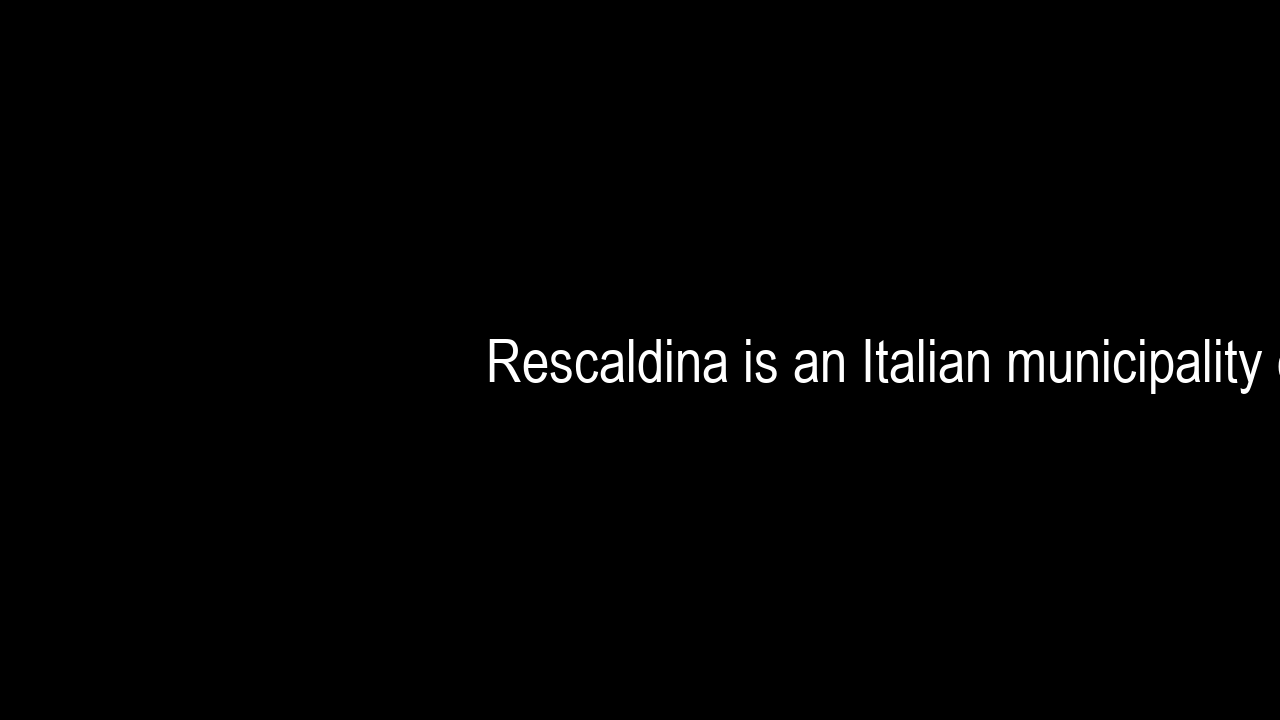
\includegraphics[width=1\textwidth,height=0.6\textwidth]{Images/Experiment/HS_big.png}
        \caption{Horizontal scroll, big text.}
        \label{fig:HS_B}
    \end{subfigure}
    
    \vspace{0.5em}
    
    % Second row
    \begin{subfigure}[b]{0.45\textwidth}
        \centering
        
\includegraphics[width=0.7\textwidth,height=0.6\textwidth]{Images/Experiment/VB_little.png}
        \caption{Vertical block, small text.}
        \label{fig:VB_L}
    \end{subfigure}
    \hfill
    \begin{subfigure}[b]{0.45\textwidth}
        \centering
        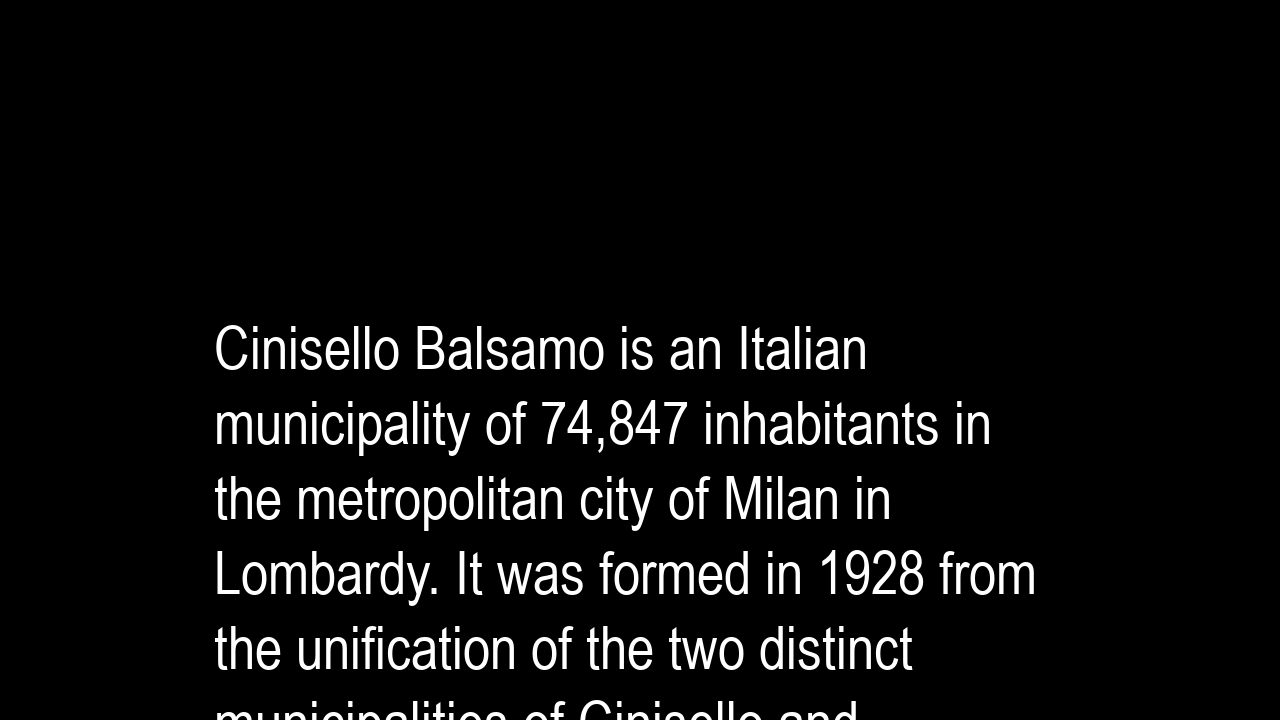
\includegraphics[width=1\textwidth,height=0.6\textwidth]{Images/Experiment/VB_big.png}
        \caption{Vertical block, big text.}
        \label{fig:VB_B}
    \end{subfigure}

    \caption{The different types of animations.}
    \label{fig:anims}
\end{figure}

The figure \ref{fig:anims} provides a representation of the two types of animations employed in the study. 
Each animation type was implemented at two distinct speeds and with two font sizes, resulting in a total of eight unique animation conditions.
\FloatBarrier

\section{Captured Eye Tracking Features}

In the present study, the set of ocular features was recorded using the GazePoint GP3\_HD eye tracker, which outputs a wide range of parameters designed to characterize visual behavior with both spatial and physiological precision. 
These features, according to [90], can be organized into several functional categories, namely fixation parameters, raw gaze coordinates, corneal reflection and pupil metrics, three-dimensional eye position, pupil dynamics, and blink-related measures. 
Each category not only describes a specific aspect of eye activity but also provides potential discriminative cues for biometric modeling.

The first group of features concerns fixations, which are intervals in which the eyes remain relatively stable on a spatial location, thereby enabling information intake and cognitive processing. 
The GP3\_HD eye tracker provides normalized screen coordinates of each fixation (FPOGX, FPOGY), which indicate the point of regard on the display. 
Alongside this spatial information, the system records the onset time of the fixation (FPOGS), its duration (FPOGD), and a unique identifier (FPOGID) for reference across the data stream. 
An additional validity flag (FPOGV) specifies the confidence of the measurement. 
Fixation duration is particularly important, as longer fixations are often associated with increased cognitive load or the processing of more complex visual material, while shorter ones may indicate scanning behavior. 
The spatial distribution of fixations across the screen, in turn, reflects attentional allocation and search strategies. 
Together, these measures provide a temporal and spatial fingerprint of how an individual interacts with visual stimuli.

Complementing the fixation measures are raw gaze coordinates, which provide the instantaneous location of the eyes on the screen without aggregation into fixation events. 
These are reported separately for the left (LPOGX, LPOGY, LPOGV) and right eyes (RPOGX, RPOGY, RPOGV), as well as for a binocular average (BPOGX, BPOGY, BPOGV). 
By distinguishing between monocular and binocular tracking, the system allows for evaluation of convergence behavior (i.e., how well the two eyes align on a target) as well as interocular differences, which may emerge from physiological asymmetries or small errors in ocular coordination. 
The binocular values represent a fused estimate of the point of regard, often more stable than monocular readings, but the monocular data themselves may carry subtle inter-eye differences that are individual-specific and thus of biometric relevance.

The third group of features relates to corneal reflection and pupil properties, which are detected by the infrared illumination system of the tracker. 
For each eye, the GP3\_HD eye tracker reports the estimated coordinates of the pupil center on the image plane (LPCX, LPCY for the left eye; RPCX, RPCY for the right eye), along with values describing pupil diameter and pupil size (LPD, LPS for the left eye; RPD, RPS for the right eye). 
Each of these measurements is associated with a validity flag (LPV, RPV), indicating whether the tracking conditions were sufficient for reliable recording. 
Pupil size is not static: it responds dynamically to changes in illumination, but is also modulated by cognitive and affective processes such as attention, emotional arousal, and mental workload. 
These fluctuations are partially involuntary, making them difficult to consciously manipulate, and thus potentially stable individual signatures. 
In addition, the spatial estimation of the pupil center contributes to precise gaze localization, while differences in pupil metrics across individuals can form part of a biometric profile.

Beyond two-dimensional gaze data, the GP3\_HD eye tracker also captures three-dimensional eye position features, reporting the x-, y-, and z-coordinates of each eye relative to the eye tracker (LEYEX, LEYEY, LEYEZ for the left eye; REYEX, REYEY, REYEZ for the right eye). 
The x and y values provide lateral and vertical offsets, while the z coordinate specifies the distance between the eye and the tracker, effectively measuring head-to-screen distance. 
These measures are particularly valuable because they reveal natural head movements, posture adjustments, or minor asymmetries in eye alignment. 
While such variability might traditionally be considered noise, in the context of biometrics, these natural tendencies may carry person-specific information. 
For example, an individual may habitually lean closer to or further from the screen, or present consistent horizontal offsets due to ocular dominance.

Closely related to pupil size are the pupil diameter dynamics, reported as LPUPILD and RPUPILD for the left and right eyes, each paired with validity indicators (LPUPILV, RPUPILV). 
These values offer fine-grained recordings of moment-to-moment changes in pupil diameter, complementing the more general pupil size parameters described earlier. 
Unlike fixation duration or gaze coordinates, which directly reflect attentional allocation, pupil dynamics provide a physiological signal that is largely involuntary and influenced by a combination of environmental, cognitive, and emotional factors.
The stability of these responses across repeated sessions, combined with their resistance to voluntary control, makes them a promising source of biometric information.

Finally, the dataset includes blink-related features, which capture involuntary eyelid closures that briefly interrupt gaze tracking. 
For each blink, the GP3\_HD eye tracker assigns a unique identifier (BKID), records its duration (BKDUR), and stores the minimum pupil size observed during the event (BKPMIN), which reflects the degree of occlusion. 
Blink dynamics are an integral part of ocular behavior, influenced by ocular physiology, fatigue levels, environmental factors, and cognitive state. 
However, inter-individual variability in blink frequency, duration, and regularity has been documented, suggesting that blinking patterns may themselves provide discriminative information. 
Importantly, because blinks are largely automatic and difficult to consciously regulate in a consistent manner, they can serve as a robust biometric trait resistant to intentional manipulation.

Taken together, the features recorded by the GP3\_HD eye tracker provide a comprehensive view of ocular activity. 
These measurements span spatial aspects of gaze location, temporal aspects of fixations and blinks, as well as physiological characteristics related to pupil dynamics and three-dimensional eye positioning.
While some features directly represent visual exploration of stimuli (e.g., gaze coordinates, fixation positions), others capture involuntary physiological responses (e.g., pupil size fluctuations, blink dynamics) or natural head/eye geometry (3D coordinates). 
The integration of these diverse signals is particularly valuable in a biometric context, as it enables the system to combine behavioral and physiological aspects of eye activity, thereby enhancing robustness, discriminative power, and resistance to spoofing.

\section{Dataset creation}

In this section, we describe the methodology employed to process the gaze-related features introduced in the previous chapter and transform them into the analytical features of the dataset. 
It is important to note from the outset that the raw gaze coordinates along the x and y axes were not included as direct features. 
This decision stems from the absence of a calibration procedure, which is intentional. 
The aim is to design a system suitable for practical, everyday applications where calibration may not be feasible. 
While this approach enhances usability and applicability in real-world scenarios, it comes at the cost of a slight reduction in the precision of gaze coordinate measurements.
In this study, a total of 83 features were derived from the raw gaze and pupil data recorded by the GazePoint GP3\_HD eye tracker. 

\subsection[Fixation-Based Features (f0–f10)]{Fixation-Based Features (\(f_0\)–\(f_{10}\))}

Fixations are periods during which the gaze remains relatively stable, enabling detailed visual processing of stimuli. 
This group of features captures both the frequency and statistical properties of fixation durations.  

Feature \(f_0\) represents the total number of fixations recorded during a trial for each animation, reflecting the frequency with which gaze stabilization occurs.  

All remaining fixation-based features (\(f_1\)–\(f_{10}\)) are derived from fixation durations, which are calculated from the relative gaze feature \(\mathrm{FPOGD}\) for each fixation's unique identifier (\(\mathrm{FPOGID}\)). 
Statistical descriptors of these durations provide insights into attentional control and scanning behavior:

\begin{itemize}
    \item \(f_1\) — \textbf{Minimum fixation duration}: The shortest fixation duration in the trial, indicating rapid scanning behavior.
    \item \(f_2\) — \textbf{Maximum fixation duration}: The longest fixation duration, showing sustained attention to a specific location.
    \item \(f_3\) — \textbf{Arithmetic mean fixation duration}: Average fixation time, representing typical gaze stability.
    \item \(f_4\) — \textbf{Geometric mean fixation duration}: A measure of central tendency less sensitive to extreme values, useful for skewed distributions.
    \item \(f_5\) — \textbf{Median fixation duration}: Middle value of fixation durations, robust against outliers.
    \item \(f_6\) — \textbf{Standard deviation fixation duration}: Variability in fixation times across the trial.
    \item \(f_7\) — \textbf{Median absolute deviation fixation duration}: Robust measure of variability, less influenced by extreme durations.
    \item \(f_8\) — \textbf{Skewness fixation duration}: Asymmetry in the distribution of fixation durations.
    \item \(f_9\) — \textbf{Interquartile range fixation duration}: Dispersion between the 25th and 75th percentile, excluding extremes.
    \item \(f_{10}\) — \textbf{Kurtosis fixation duration}: Describes the "peakedness" of the fixation duration distribution.
\end{itemize}


\subsection[Fixation Distance Features (f11–f20)]{Fixation Distance Features (\(f_{11}\)–\(f_{20}\))}

These features quantify spatial distances between consecutive fixations, characterizing gaze exploration and scanning behavior.  

Distances are computed from the normalized gaze coordinates, \(\mathrm{FPOGX}\) and \(\mathrm{FPOGY}\), for each fixation. 
For each pair of consecutive fixations \((x_i, y_i)\) and \((x_{i+1}, y_{i+1})\), the Euclidean distance \(d_i\) is calculated as:

\[
d_i = \sqrt{(x_{i+1} - x_i)^2 + (y_{i+1} - y_i)^2}.
\]

These distances form a distribution for each trial, from which statistical descriptors are extracted to capture the spatial patterns of gaze movement:

\begin{itemize}
    \item \(f_{11}\) — \textbf{Minimum distance}: Smallest shift between consecutive fixations, indicating very local gaze changes.
    \item \(f_{12}\) — \textbf{Maximum distance}: Largest shift, reflecting broad scanning movements.
    \item \(f_{13}\) — \textbf{Arithmetic mean distance}: Average spatial shift, representing typical scanning magnitude.
    \item \(f_{14}\) — \textbf{Geometric mean distance}: Central tendency less influenced by extreme distances.
    \item \(f_{15}\) — \textbf{Median distance}: Middle value of fixation-to-fixation distances.
    \item \(f_{16}\) — \textbf{Standard deviation distance}: Variability of spatial shifts.
    \item \(f_{17}\) — \textbf{Median absolute deviation distance}: Robust measure of spatial variability.
    \item \(f_{18}\) — \textbf{Skewness distance}: Asymmetry of the distance distribution.
    \item \(f_{19}\) — \textbf{Interquartile range distance}: Dispersion measure excluding extreme values.
    \item \(f_{20}\) — \textbf{Kurtosis distance}: Shape of the spatial distance distribution.
\end{itemize}

\subsubsection[Saccade Speed Features (f21–f30)]{Saccade Speed Features (\(f_{21}\)–\(f_{30}\))}

Saccades are rapid eye movements occurring between fixations, responsible for shifting the line of sight toward new visual targets. 
To quantify their dynamics, saccade speeds are computed using the normalized gaze coordinates \(\mathrm{FPOGX}\) and \(\mathrm{FPOGY}\), combined with temporal markers from the gaze data. 
For each pair of successive fixation points, the Euclidean distance between consecutive gaze positions is first determined. 
The corresponding time interval is calculated as the difference in starting times of consecutive fixations, \(\mathrm{FPOGS}_{i+1} - \mathrm{FPOGS}_i\), adjusted by subtracting the duration of the first fixation \(\mathrm{FPOGD}_i\). 
This ensures that the interval reflects only the transition time between fixations. 
Saccade speed for the transition is then defined as:

\[
v_i = \frac{\sqrt{(x_{i+1} - x_i)^2 + (y_{i+1} - y_i)^2}}{t_{i+1} - t_i - d_i},
\]

where \((x_i, y_i)\) and \((x_{i+1}, y_{i+1})\) denote successive fixation coordinates, \(t_i\) the start time of fixation \(i\), and \(d_i\) its duration. 
This procedure yields a distribution of saccade speeds for each trial, summarized through descriptive statistics.

\begin{itemize}
    \item \(f_{21}\) — Minimum saccade speed: The lowest velocity observed among saccades, indicating the slowest gaze transitions.
    \item \(f_{22}\) — Maximum saccade speed: The highest velocity recorded, reflecting the most abrupt shifts in gaze.
    \item \(f_{23}\) — Arithmetic mean saccade speed: Average speed across all saccades within the trial.
    \item \(f_{24}\) — Geometric mean saccade speed: Central tendency of saccade speeds, less influenced by extreme values.
    \item \(f_{25}\) — Median saccade speed: The middle speed value, robust against outlier influence.
    \item \(f_{26}\) — Standard deviation saccade speed: Variability of saccadic velocities across the trial.
    \item \(f_{27}\) — Median absolute deviation saccade speed: Robust measure of variation in saccade dynamics.
    \item \(f_{28}\) — Skewness saccade speed: Asymmetry of the saccade speed distribution, indicating bias toward slower or faster movements.
    \item \(f_{29}\) — Interquartile range saccade speed: Spread of saccade velocities within the 25th–75th percentile range.
    \item \(f_{30}\) — Kurtosis saccade speed: Peakedness or tail heaviness of the speed distribution.
\end{itemize}

\subsection[Scanpath Feature (f31)]{Scanpath Feature (\(f_{31}\))}

The scanpath length provides a global measure of the total extent of visual exploration during a trial. 
It is computed as the cumulative sum of Euclidean distances between consecutive fixation points, based on their normalized screen coordinates \(\mathrm{FPOGX}\) and \(\mathrm{FPOGY}\). 
Formally, for fixation points \((x_i, y_i)\), the scanpath length \(L\) is:

\[
L = \sum_{i=1}^{N-1} \sqrt{(x_{i+1} - x_i)^2 + (y_{i+1} - y_i)^2},
\]

where \(N\) is the total number of fixation points. 

\begin{itemize}
    \item \(f_{31}\) — Scanpath length: Total cumulative distance of gaze movements during a trial, representing the overall extent of visual exploration.
\end{itemize}


\subsection[Pupil Diameter Features (f32–f51)]{Pupil Diameter Features (\(f_{32}\)–\(f_{51}\))}

Pupil diameter is a physiological indicator influenced by luminance, cognitive load, and emotional state. 
Values were extracted separately for the left and right eyes (\(\mathrm{LPD}\) and \(\mathrm{RPD}\)), including only valid samples (\(\mathrm{LPV} = 1\) or \(\mathrm{RPV} = 1\)). 
For each eye, pupil diameters across the trial were summarized using descriptive statistics, generating two parallel groups of features: \(f_{32n}\)--\(f_{41n}\) for the left eye and \(f_{42n}\)--\(f_{51n}\) for the right eye.

\begin{itemize}
    \item \(f_{32}, f_{42}\) — Minimum pupil diameter
    \item \(f_{33}, f_{43}\) — Maximum pupil diameter
    \item \(f_{34}, f_{44}\) — Arithmetic mean pupil diameter
    \item \(f_{35}, f_{45}\) — Geometric mean pupil diameter
    \item \(f_{36}, f_{46}\) — Median pupil diameter
    \item \(f_{37}, f_{47}\) — Standard deviation pupil diameter
    \item \(f_{38}, f_{48}\) — Median absolute deviation pupil diameter
    \item \(f_{39}, f_{49}\) — Skewness pupil diameter
    \item \(f_{40}, f_{50}\) — Interquartile range pupil diameter
    \item \(f_{41}, f_{51}\) — Kurtosis pupil diameter
\end{itemize}

\subsection[Pupil Diameter Ratio Features (f52–f61)]{Pupil Diameter Ratio Features (\(f_{52}\)–\(f_{61}\))}

The ratio between left and right pupil diameters (\(\mathrm{LPD}/\mathrm{RPD}\)) was computed using valid samples from both eyes (\(\mathrm{LPV} = 1\) and \(\mathrm{RPV} = 1\)). 
Descriptive statistics summarize the distribution across the trial, yielding features \(f_{52n}\)--\(f_{61n}\).

\begin{itemize}
    \item \(f_{52}\) — Minimum ratio
    \item \(f_{53}\) — Maximum ratio
    \item \(f_{54}\) — Arithmetic mean ratio
    \item \(f_{55}\) — Geometric mean ratio
    \item \(f_{56}\) — Median ratio
    \item \(f_{57}\) — Standard deviation ratio
    \item \(f_{58}\) — Median absolute deviation ratio
    \item \(f_{59}\) — Skewness ratio
    \item \(f_{60}\) — Interquartile range ratio
    \item \(f_{61}\) — Kurtosis ratio
\end{itemize}

\subsection[Pupil Diameter Difference Features (f62–f70)]{Pupil Diameter Difference Features (\(f_{62}\)–\(f_{70}\))}

Direct differences between left and right pupil diameters were computed as \(D = \mathrm{LPD} - \mathrm{RPD}\), using only valid samples. 
Descriptive statistics were then extracted, resulting in features \(f_{62n}\)--\(f_{70n}\). The geometric mean is excluded due to possible negative values.

\begin{itemize}
    \item \(f_{62}\) — Minimum difference
    \item \(f_{63}\) — Maximum difference
    \item \(f_{64}\) — Arithmetic mean difference
    \item \(f_{65}\) — Median difference
    \item \(f_{66}\) — Standard deviation difference
    \item \(f_{67}\) — Median absolute deviation difference
    \item \(f_{68}\) — Skewness difference
    \item \(f_{69}\) — Interquartile range difference
    \item \(f_{70}\) — Kurtosis difference
\end{itemize}

\subsection[Blink Features (f71–f74)]{Blink Features (\(f_{71}\)–\(f_{74}\))}

Blink features were extracted from identifiers (\(\mathrm{BKID}\)) and durations (\(\mathrm{BKDUR}\)).

\begin{itemize}
    \item \(f_{71}\) — Number of blinks
    \item \(f_{72}\) — Mean blink duration
    \item \(f_{73}\) — Minimum blink duration
    \item \(f_{74}\) — Maximum blink duration
\end{itemize}

\subsection[Directional Movement Features (f75–f82)]{Directional Movement Features (\(f_{75}\)–\(f_{82}\))}

Directional movements capture horizontal and vertical gaze displacements:

\begin{itemize}
    \item \(f_{75}\) — Total upward distance (\(\Delta y < 0\))
    \item \(f_{76}\) — Total downward distance (\(\Delta y > 0\))
    \item \(f_{77}\) — Total leftward distance (\(\Delta x < 0\))
    \item \(f_{78}\) — Total rightward distance (\(\Delta x > 0\))
    \item \(f_{79}\) — Number of upward transitions
    \item \(f_{80}\) — Number of downward transitions
    \item \(f_{81}\) — Number of leftward transitions
    \item \(f_{82}\) — Number of rightward transitions
\end{itemize}

\newpage

\chapter{Machine Learning Analysis}

This section presents the machine learning analysis conducted on the collected data, which has been represented through the diverse set of features described in the previous section. 
Given that the domain of behavioral biometrics based on dynamic text remains largely unexplored, our study also investigates the feasibility of performing user identification. 

It is well established that biometric identification based on behavioral signals often achieves limited performance, making it unsuitable for reliable use in soft biometric applications. 
Nevertheless, prior research has shown that certain modalities, such as keystroke dynamics [9], represent notable exceptions. 
Accordingly, our first objective is to assess whether gaze- and pupil-based features in our setting also exhibit such exceptionality in the identification task. 

In addition to this evaluation, the identification analysis is leveraged as a methodological step to optimize hyperparameters and to determine the most informative subsets of features via the SelectKBest method [91]. 
The insights obtained from this stage are subsequently applied to the verification analysis, which constitutes the core of our biometric evaluation. 
Specifically, by transferring the optimized hyperparameters and reduced feature sets from the identification task, we significantly lower the computational cost of verification. 
This step is crucial, as verification requires training a separate model for each individual in the dataset, and performing hyperparameter optimization for every subject would otherwise lead to prohibitive computational demands.

In our analysis, we employ seven different machine learning classifiers to construct and evaluate predictive models.
As an initial step, we used the Naïve Bayes classifier to obtain a preliminary understanding of the potential performance that could be achieved.
However, due to its strong assumption of feature independence, which is rarely satisfied in practice, this model is utilized solely for exploratory purposes.
Consequently, Naïve Bayes results are not included in the main performance tables, as the classifier is primarily used for a rapid baseline estimation, and its performance is typically inferior to more advanced methods.

Among the classifiers employed in this study, the k-Nearest Neighbors (kNN) algorithm [94] represents a well-established and widely used method across various application domains.
One of the principal strengths of k-NN lies in its simplicity and interpretability, making it an effective baseline model before the adoption of more complex techniques.
It often provides satisfactory performance without extensive parameter tuning, which makes it particularly suitable for exploratory analysis.
While the construction of a k-NN model is computationally efficient, prediction time can become relatively slow when dealing with large datasets, either in terms of the number of features or the number of samples [93].

The next classifier employed is Logistic Regression [95], which is widely used due to its simplicity, interpretability, and efficiency. 
One of its main advantages is that it is easy to implement and does not require strong assumptions about the distribution of the classes in the feature space. 
Moreover, Logistic Regression can be naturally extended to handle multiple classes through multinomial regression, providing a probabilistic interpretation of class predictions that is both intuitive and informative.
However, the primary limitation of Logistic Regression lies in its assumption of linearity between the independent variables and the log odds of the dependent variable. 
As a result, it can only model linear decision boundaries and therefore struggles to capture more complex, nonlinear relationships that may exist within the data [96].

To proceed we used SVC [97] and one of its variants Nusvc [98].
According to [93], Kernelized Support Vector Machines (SVMs) are highly effective models capable of learning complex decision boundaries, even with few features. 
They perform well on both low- and high-dimensional data but scale poorly with the number of samples. 
While datasets up to around 10,000 samples are manageable, larger ones can cause significant runtime and memory issues. 
Moreover, SVMs require careful data preprocessing and precise parameter tuning to achieve optimal performance.
Unlike SVC, which relies on the parameter C to balance the trade-off between maximizing the margin and minimizing classification errors, NuSVC introduces the parameter v (nu).
This parameter defines an upper bound on the proportion of training errors and a lower bound on the proportion of support vectors. 
As a result, NuSVC offers a more interpretable and direct means of controlling model complexity and the number of support vectors involved in the decision function [99].

The next classifier is one of the most well-known and widely used: Random Forest [100].
Random forests are powerful machine learning methods for both regression and classification, requiring minimal parameter tuning and no data scaling. 
They retain the strengths of decision trees while overcoming many of their limitations. 
However, their complexity—arising from combining numerous deep trees—reduces interpretability, making single decision trees preferable when a simple, visual explanation of the decision process is needed [93].

Finally, the last classifier used is the multilayer perceptron (MLP) [101]. 
Neural networks have regained prominence in machine learning due to their ability to capture complex patterns from large datasets. 
With sufficient data, computation, and parameter tuning, they often outperform other algorithms in both classification and regression tasks. 
However, they require extensive training time, careful data preprocessing, and are best suited for homogeneous data [93]. 

The classifiers presented above will be employed throughout the analysis. 
A single classifier is not used because, in machine learning, there is no universally best algorithm.
In fact performance depends on the characteristics of the data and the specific problem being addressed.

As previously stated, the first part of the analysis focuses on the identification problem. 
This phase employs two distinct data-splitting strategies to create training and testing sets. 
The first is the classic random split using 80\% of the data for the train set and 20\% for the test set.
The second is a session-based split, where data from the first two sessions (S1 and S2) form the training set, and data from the third session (S3) is used as the test set.
Initially, a general identification will be performed using the entire dataset, both with and without feature selection, to evaluate any potential improvements in performance.
An analysis involving every single animation taken singularly is then performed to assess which is the best-performing animation and see if a single animation can be used for identification purposes.
This analysis is divided into two types, based on the data used in the training set.
The first method is called Single Train (ST), where the model is trained and tested on data from a single animation.
While the second approach is called Full Train (FT), where the model is trained on data from all animations combined and tested on a single animation.
The latter method has been used in previous studies and, in some cases, achieved better results due to the larger amount of training data. 
However, in other cases, performance worsened because the inclusion of all animations introduced confusion between different data distributions.

Afterward, we proceed to the verification phase, which represents the main objective of this work.
In this stage, we employ only the session-based split, applied in the same manner as in the identification analysis.
This choice reflects a more realistic, real-world scenario, where user verification occurs across different sessions.
Similar to the identification phase, we first conduct a global analysis using the entire dataset across all animations, both with and without feature selection, to obtain a general overview of the achievable performance.
Subsequently, we focus on single-animation analyses, maintaining the two training strategies previously adopted for identification.
However, this part introduces an additional division.
Specifically, we evaluate two modes, st and ft, to compare a standard verification approach with one that uses only the best-performing model for testing. 
These modes will be discussed in detail in the dedicated chapter.
For all these configurations, we also performed an open-set analysis to evaluate how the system responds when an unregistered and previously unseen user attempts authentication.
Finally, to complete the verification analysis, we conducted a temporal scaling experiment, reducing the duration of all animations. 
The objective was to assess how the best-performing animation behaves when using only the first 10 or 5 seconds instead of the full 15-second duration.

Finally, we perform a comparative analysis between identification and verification using the full dataset, rather than single animations, in order to assess the performance differences between static and dynamic text under similar experimental conditions.

\section{Identification}
The first analysis focuses on identification.
In this case, a multiclass evaluation is performed to assess the application's performance in this domain. 
Although this is not the final objective of the study, evaluating identification performance remains important, as previous applications have demonstrated promising results in this area.
Furthermore, this analysis serves to identify the optimal combination of hyperparameters and to select the most relevant features, which will later be used in the subsequent verification phase.

\subsection{Identification without feature selection}
\label{subsec:id_fs_ch}

We begin the identification analysis using the entire dataset, without distinguishing between different animations.
In this initial phase, feature selection through SelectKBest [91] is intentionally omitted, as the objective is to establish a baseline reference. 
These results will serve as a comparison point to evaluate potential improvements obtained when applying feature selection in subsequent analyses.
The program goal is to use two different types of splits: random split and session split.

The random split is performed using the train\_test\_split function [102], where 80\% of the dataset is randomly selected to form the training set, and the remaining 20\% is used as the test set.
To ensure balanced representation across individuals, stratification based on the tester identifier is applied.
This guarantees that approximately 80\% of each participant's data is included in the training set, while the remaining 20\% is allocated to the test set, maintaining consistent class proportions across both subsets.
To minimize the randomness inherent in this approach, the procedure was repeated ten times, and the results were averaged across all runs.
This repetition reduces the impact of particularly favorable or unfavorable data splits that could otherwise bias the performance evaluation.

The session-based split corresponds to the three recording sessions conducted on different days. 
This design was chosen primarily to minimize the influence of temporary conditions such as fatigue or momentary distraction, ensuring that the data reflect a more stable and representative ocular behavior. 
Moreover, performing the recordings on separate days allows us to average out day-to-day variability. 
The second motivation for this setup is methodological: the data from the first two sessions (S1 and S2) are used to train the model, while the third session (S3) serves as the test set, enabling an evaluation of the model's generalization capability across sessions.

A hyperparameter tuning procedure was implemented using a pipeline [103] composed of three main stages.
The first stage employs the SimpleImputer [105] to handle missing values by replacing them with the mean of the corresponding feature column. 
The second stage performs feature scaling, tested with three different normalization methods: MinMaxScaler [106], StandardScaler [107], and RobustScaler [108]. 
Finally, the third stage involves hyperparameter optimization, using the parameter grids reported in Table \ref{tab:pg_nofs} and GridSearchCV [104]. 
It is important to note that each time a GridSearchCV strategy was applied to determine the optimal hyperparameters, the complete pipeline configuration was consistently employed. 
The hyperparameter optimization was conducted using a 5-fold cross-validation procedure (\texttt{cv = 5}), in which the training data were divided into five equally sized folds. 
In each iteration, four folds were used for model training and the remaining one for validation. 
This process was repeated five times so that every fold served once as the validation set, and the resulting performance metrics were averaged to obtain a more reliable and unbiased estimate of the model's performance.

We're now ready to present the results obtained during this analysis.

\begin{table}[ht]
    \centering
    \caption{Identification results without feature selection.} % appears above
    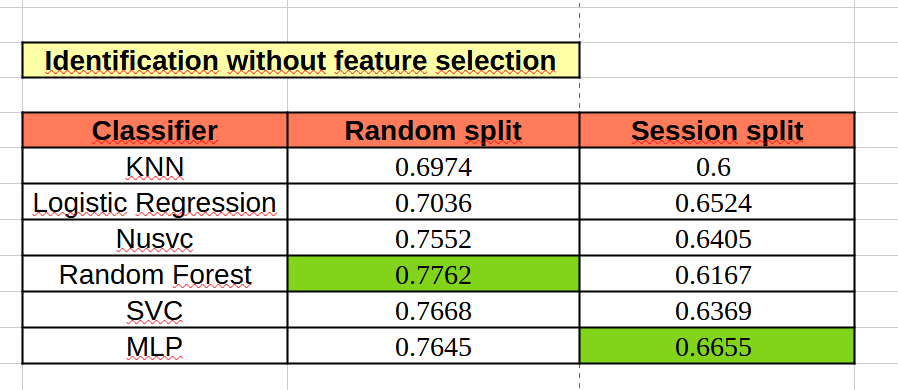
\includegraphics[width=0.6\textwidth]{Images/Results/Identification/nofs.png}
    \label{tab:id_nofs}
\end{table}


The Table \ref{tab:id_nofs} illustrates that, for the random split type, the best performance is achieved by the Random Forest classifier, yielding an accuracy of 77.62\%.
In contrast, for the session split type, the highest accuracy is obtained by the Multilayer Perceptron (MLP) model, with a value of 66.55\%.

A notable performance drop is observed when transitioning from the random split to the session split. 
This decline is expected and can be attributed to the reduced amount of training data available in the session split scenario. 
Specifically, the random split allocates 80\% of the data to the training set, whereas the session split allocates only 66.6\%.
Moreover, the random split introduces a potential data leakage issue, as samples from the same session may appear in both the training and testing sets. 
This overlap provides the model with indirect information about the test data, thereby inflating performance compared to the session split, where such leakage is avoided.
\FloatBarrier

\subsection{Identification with feature selection.}

We now proceed to perform the identification analysis with an additional step: feature selection.
The overall procedure and implementation remain identical to those described in Appendix \ref{subsec:id_fs_ch}.
In particular two data split strategies were used, random and session, together with GridSearchCV for hyperparameter optimization.
The main difference lies in the inclusion of the feature selection stage, illustrated in Table \ref{tab:pg_fs}. 
Specifically, we employed the SelectKBest method[91] to identify the subset of features (k) that yielded the highest mean cross-validation accuracy during the grid search.
This approach not only enhances model interpretability but also reduces the dimensionality of the feature space, thereby potentially improving generalization performance.

\begin{table}[ht]
    \centering
    \caption{Identification results with feature selection.}
    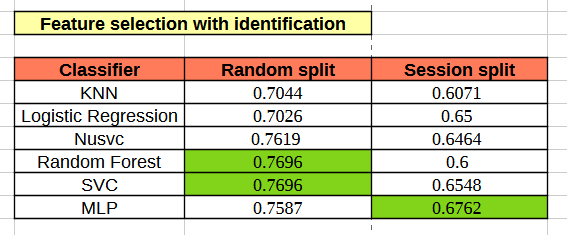
\includegraphics[width=0.6\textwidth]{Images/Results/Identification/fs.png}
    \label{tab:id_fs}
\end{table}


The Table \ref{tab:id_fs} presents the results obtained from this analysis.
For the random split type, the Random Forest classifier remains the best performer, achieving an accuracy of 76.69\%.
This represents a slight decrease compared to the accuracy of 77.62\% obtained without the feature selection step, corresponding to a reduction of 13 features (from 83 to 70).
Interestingly, the Support Vector Classifier (SVC) achieved the same accuracy of 76.69\% using the reduced feature set of 70 features, matching the performance of the Random Forest under these conditions.

For the session split, a modest improvement was observed with the Multilayer Perceptron (MLP) classifier, whose accuracy increased from 66.55\% to 67.62\% when using only 70 features.

The number of selected features, along with their corresponding identities, is presented in Appendix \ref{subsec:id_fs_k}.
\begin{table}[htbp]
\centering
\scriptsize
\setlength{\tabcolsep}{3pt}
\caption{Top 30 features for Identification with feature selection ranked by cumulative F-score.}
\label{tab:top30_id}
\begin{tabular}{lll}
\toprule
\textbf{Feature ID} & \textbf{Feature name} & \textbf{Cumulative F-score} \\
\midrule
f44 & Arithmetic mean right pupil diameter & 2777.22 \\
f45 & Geometric mean right pupil diameter & 2724.38 \\
f46 & Median right pupil diameter & 2658.24 \\
f34 & Arithmetic mean left pupil diameter & 2482.82 \\
f35 & Geometric mean left pupil diameter & 2443.10 \\
f36 & Median left pupil diameter & 2384.14 \\
f64 & Arithmetic mean difference between left and right pupil diameter & 1734.38 \\
f65 & Median difference between left and right pupil diameter & 1697.57 \\
f33 & Maximum left pupil diameter & 1644.71 \\
f43 & Maximum right pupil diameter & 1561.86 \\
f55 & Geometric mean ratio between left and right pupil diameter & 1139.40 \\
f56 & Median ratio between left and right pupil diameter & 1125.79 \\
f54 & Arithmetic mean ratio between left and right pupil diameter & 1065.89 \\
f71 & Number of blinks & 760.39 \\
f52 & Minimum ratio between left and right pupil diameter & 599.55 \\
f62 & Minimum difference between left and right pupil diameter & 529.04 \\
f58 & Median absolute deviation ratio between left and right pupil diameter & 437.26 \\
f60 & Interquartile range ratio between left and right pupil diameter & 410.47 \\
f67 & Median absolute deviation difference between left and right pupil diameter & 385.03 \\
f69 & Interquartile range difference between left and right pupil diameter & 374.81 \\
f66 & Standard deviation difference between left and right pupil diameter & 357.18 \\
f63 & Maximum difference between left and right pupil diameter & 340.73 \\
f39 & Skewness left pupil diameter & 250.94 \\
f53 & Maximum ratio between left and right pupil diameter & 234.36 \\
f37 & Standard deviation left pupil diameter & 228.57 \\
f57 & Standard deviation ratio between left and right pupil diameter & 227.71 \\
f49 & Skewness right pupil diameter & 223.79 \\
f80 & Number of movements in descending direction & 210.63 \\
f42 & Minimum right pupil diameter & 196.55 \\
f32 & Minimum left pupil diameter & 196.55 \\
\bottomrule
\end{tabular}
\end{table}

Table \ref{tab:top30_id} displays the top 30 features selected across the entire analysis.
These features were ranked according to their cumulative F-score, aggregated across all classifiers and session splits.
Each time a feature appeared during the selection process, its F-score was added to an accumulator. 
If the same feature appeared again in subsequent analyses, its score was added cumulatively to the previous total.
As shown in the table, the top 10 positions are predominantly occupied by pupil-related features, either referring to a single eye or derived from ratios or differences between the two eyes.

{\raggedright
In contrast, Table \ref{tab:ns_id} displays the set of features that were never selected in any model or split type.
We can observe that many of these are saccade speed features, along with two distance-between-consecutive-fixations features.
Interestingly, the kurtosis ratio between left and right pupil diameter is also never selected, despite pupil diameter being among the best features. 
This suggests that kurtosis may not be a representative metric in this context.
\par}

\begin{table}[H]
\centering
\small
\setlength{\tabcolsep}{4pt} % same as top 30 table
\caption{List of features never selected in Identification with feature selection.}
\label{tab:ns_id}
\begin{tabular}{lll}
\toprule
\textbf{Feature ID} & \textbf{Feature name} & \textbf{Description} \\
\midrule
f11 & Minimum distance between consecutive fixations & Saccade-related metric \\
f16 & Standard deviation distance between consecutive fixations & Saccade-related metric \\
f21 & Minimum saccade speed & Saccade speed metric \\
f23 & Arithmetic mean saccade speed & Saccade speed metric \\
f24 & Geometric mean saccade speed & Saccade speed metric \\
f25 & Median saccade speed & Saccade speed metric \\
f28 & Skewness saccade speed & Saccade speed metric \\
f30 & Kurtosis saccade speed & Saccade speed metric \\
f61 & Kurtosis ratio between left and right pupil diameter & Pupil diameter ratio metric \\
\bottomrule
\end{tabular}st
\end{table}
\FloatBarrier


\subsection{Identification with single animation - Single Train (ST)}
\label{subsec:id_s_st}

The main goal of this stage was to identify which animation performs best among the eight selected stimuli. 
We began with a full identification analysis to establish a general baseline of the performance achievable when using all animations together. 
Building on this, we refined the analysis to examine the performance of each animation individually. 
This refined procedure, referred to as the Single Train (ST) approach, trains the model using data from one animation only and then tests it on data from the same animation.

Two data splitting strategies were used to ensure robust evaluation. 
The first, a random split, allocates 80\% of the data for a given animation to training and the remaining 20\% to testing.
This process was stratified by tester ID to ensure a fairer distribution and was repeated ten times to reduce variability caused by random sampling.

The second, a session-based split, uses data from the first two sessions of an animation for training and the third session for testing. 
This method was executed once to simulate a real-world scenario of session progression.

The analysis was conducted through a structured pipeline composed of four sequential steps. 
First, missing values were addressed using an imputation procedure that replaced them with the mean value of each respective feature, ensuring completeness of the dataset. 
Second, a scaling step was applied to standardize the feature values, bringing them onto a comparable range and preventing scale-related bias in the model. 
Third, a feature selection process was performed, following the same methodology as in the previous analysis, to identify and retain the most informative features for the model. 
Finally, hyperparameter tuning was carried out using GridSearchCV with the parameter grid presented in Table \ref{tab:pg_fs}, optimizing the model's performance.

This analysis serves a dual purpose. 
Primarily, it evaluates the performance of each animation within the context of an identification task, providing insight into their relative effectiveness. 
Additionally, it establishes the optimal parameters for the subsequent verification analysis, which is considerably more computationally intensive as it requires constructing a separate model for each individual. 
By performing parameter tuning within the single-animation identification analysis, this process becomes significantly more efficient. 
The parameters identified through this analysis, together with the top k features selected, constitute the foundation for the verification analysis, in which feature selection determines the final set of features used for model evaluation.

\begin{table}[ht]
    \centering
    \caption{Results for identification with single animation - ST.}
    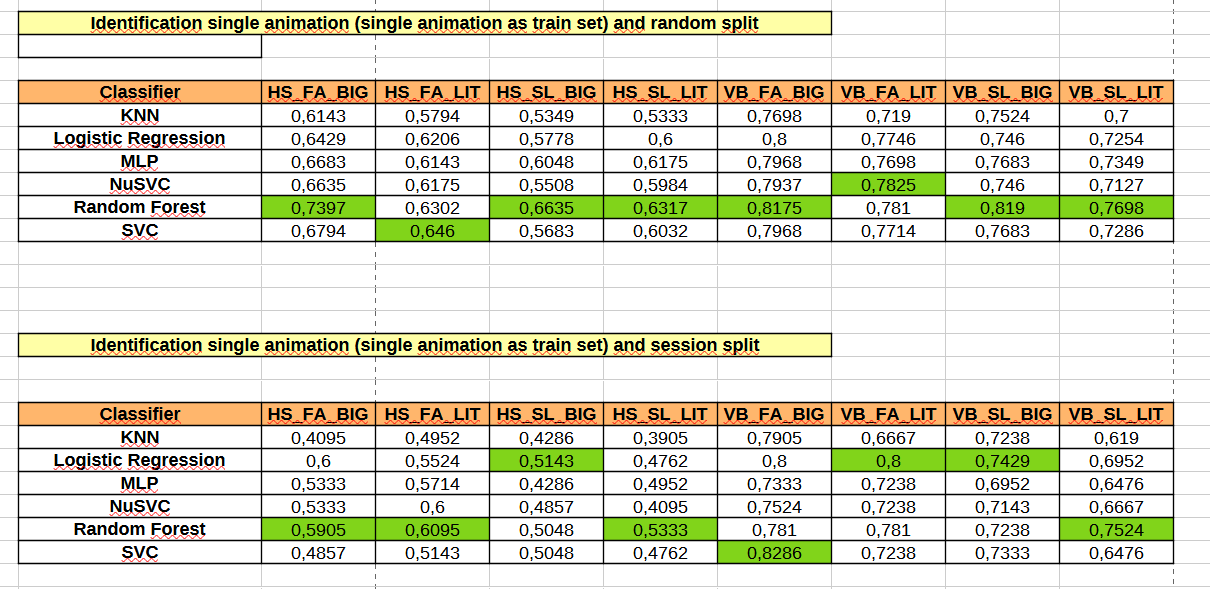
\includegraphics[width=0.8\textwidth]{Images/Results/Identification_single/single_id_st.png}
    \label{tab:id_s_st}
\end{table}

The Table \ref{tab:id_s_st} presents a comprehensive collection of the results obtained during the analysis. 
For each type of data split, the figure includes a table showing the performance of each animation using the selected classifier.

Considering the random split, the best-performing animations are VB\_SL\_BIG with an accuracy of $81.9\%$ and VB\_FA\_BIG with an accuracy of $81.75\%$.
Both of these results were achieved using the Random Forest classifiers. 
In contrast, when evaluating the session split, VB\_FA\_BIG emerges as the best performer, with accuracy increasing from $81.75\%$ to $82.86\%$ using SVC. 
This is followed by VB\_FA\_SMA, whose accuracy rises from $78.25\%$ to $80\%$, while VB\_SL\_BIG shows a notable decrease from $81.9\%$ to $74.29\%$.
These resulst were obtained with a Logistic regression classifier.

At first glance, this behaviour may seem counterintuitive, as one would generally expect performance to decrease under a session split compared to a random split. 
This expectation is based on the fact that the training set for the random split contains 80\% of the data, whereas the training set for the session split contains only 66.6\%, and in the random split samples from the same session can appear in both the training and test sets. 
However, the results reveal a more nuanced pattern: certain animations experience a drop in accuracy, particularly horizontal scroll types, while others show slight improvements despite having a smaller training set.

This improvement may be attributed to the reduced risk of overfitting when training on more distinct session data. 
By excluding samples from the same session in training and testing, the model may generalise better to unseen data, particularly in animations with more consistent and robust patterns. 
This behaviour appears to be a characteristic of dynamic text stimuli, and further evidence supporting this observation will be discussed in Appendix \ref{subsec:s_vs_d}.

\begin{table}[htbp]
\centering
\scriptsize
\setlength{\tabcolsep}{3pt}
\caption{Top 30 features for Identification single animation - ST.}
\label{tab:top30_id_s_st}
\begin{tabular}{lll}
\toprule
\textbf{Feature ID} & \textbf{Feature name} & \textbf{Cumulative F-score} \\
\midrule
f44 & Arithmetic mean right pupil diameter & 2658.73 \\
f46 & Median right pupil diameter & 2640.75 \\
f45 & Geometric mean right pupil diameter & 2626.95 \\
f34 & Arithmetic mean left pupil diameter & 2461.19 \\
f35 & Geometric mean left pupil diameter & 2430.31 \\
f36 & Median left pupil diameter & 2408.50 \\
f64 & Arithmetic mean difference between left and right pupil diameter & 2052.77 \\
f43 & Maximum right pupil diameter & 2049.28 \\
f65 & Median difference between left and right pupil diameter & 2032.88 \\
f33 & Maximum left pupil diameter & 1846.29 \\
f56 & Median ratio between left and right pupil diameter & 1452.92 \\
f55 & Geometric mean ratio between left and right pupil diameter & 1448.45 \\
f54 & Arithmetic mean ratio between left and right pupil diameter & 1386.62 \\
f67 & Median absolute deviation difference between left and right pupil diameter & 1121.41 \\
f69 & Interquartile range difference between left and right pupil diameter & 1073.47 \\
f71 & Number of blinks & 1046.55 \\
f58 & Median absolute deviation ratio between left and right pupil diameter & 963.74 \\
f78 & Total distance in absolute value in the left direction & 954.15 \\
f77 & Total distance in absolute value in the right direction & 933.19 \\
f60 & Interquartile range ratio between left and right pupil diameter & 893.48 \\
f82 & Number of movements in the ascending direction & 844.49 \\
f52 & Minimum ratio between left and right pupil diameter & 770.60 \\
f62 & Minimum difference between left and right pupil diameter & 766.01 \\
f0 & Number of fixations & 732.23 \\
f14 & Geometric mean distance between consecutive fixations & 706.63 \\
f66 & Standard deviation difference between left and right pupil diameter & 690.05 \\
f4 & Geometric mean fixation duration & 654.63 \\
f15 & Median distance between consecutive fixations & 644.81 \\
f3 & Arithmetic mean fixation duration & 643.15 \\
f80 & Number of movements in the ascending direction & 635.33 \\
\bottomrule
\end{tabular}
\end{table}

The Table \ref{tab:top30_id_s_st} presents the top 30 features identified in this analysis.
The ranking was determined by summing the F-scores of each feature across all selections and ordering them from highest to lowest.
Notably, the leaderboard is largely dominated by pupil size-related features, which appear to be highly descriptive of individual human behavior.
In contrast, the only two features that were never selected are Feature 30: Kurtosis of Saccade Speed and Feature 61: kurtosis ratio between left and right pupil diameter, suggesting that there are not particularly informative descriptors for the identification task.
\FloatBarrier

\subsection{Identification with single animation - Full Train(FT)}
\label{subsec:id_s_ft}

This type of analysis originates from previous research conducted at the University of Pavia [35], where a similar data split was employed. 
In several cases, this approach yielded better results compared to the standard Single Train(ST) version presented previously.
We also aim to evaluate this alternative approach to determine whether it yields improved or degraded performance compared to the classical procedure described in Section \ref{subsec:id_s_st}. 

The current analysis follows the same methodology as the counterpart, with one key modification: the model is trained on the entire animation dataset and tested on a single animation. 
This design intends to assess whether incorporating a larger and more diverse training set enhances the model's generalization performance, or instead introduces noise that may reduce accuracy.

As before, the first step in this program is a random “80/20” split, which partitions the dataset into training and testing subsets by selecting 80\% of the data for training and 20\% for testing, while preserving the label distribution through stratification. 
This splitting procedure is performed separately for each animation category to ensure balanced representation across classes. 
For each animation, the samples are divided so that both the training and testing sets contain data from all participants, maintaining diversity within each subset. 
The resulting training subsets from all animations are then aggregated into a single global training set, which is used to train the model, while the testing subsets are kept individually in a structured collection for per-animation evaluation. 

The session split type works in a similar way to the random spli,t but is organized by recording sessions rather than random selection. 
Specifically, for each animation, the first two sessions (S1 and S2) are collected and combined to form the training set, ensuring that the model learns from multiple recordings of each animation. 
Then, the test set for each animation is constructed exclusively from the corresponding third session (S3) data. 
Each of these animation-specific test sets is used to evaluate the model individually, allowing a detailed assessment of performance for each animation under unseen session conditions.

\begin{table}[ht]
    \centering
    \caption{Results for identification with single animation - FT.}
    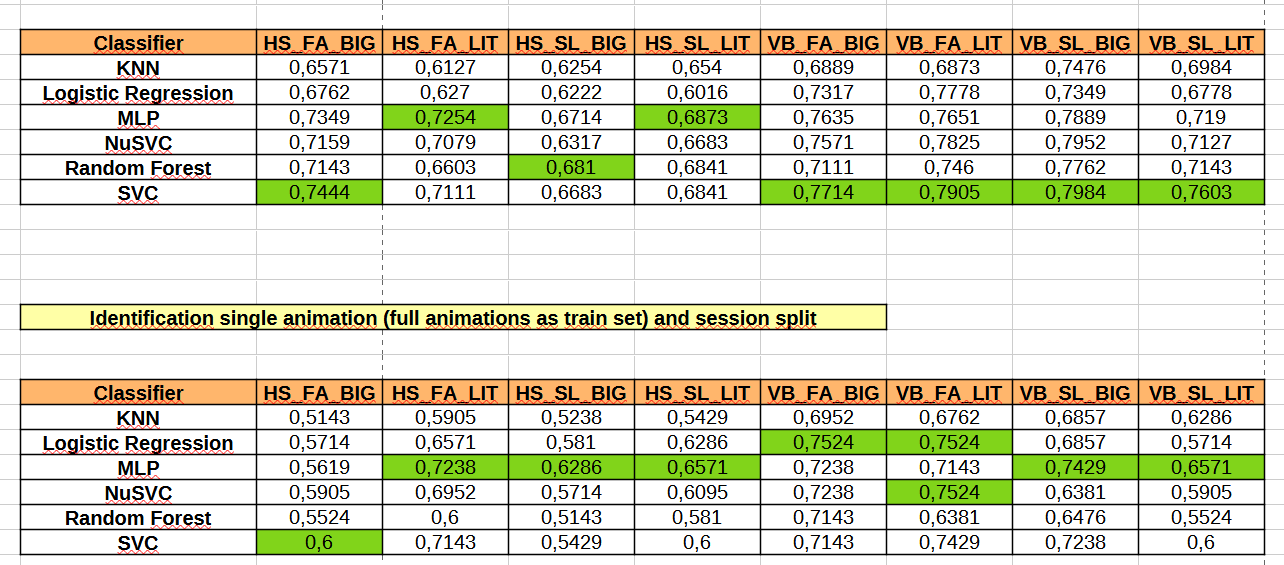
\includegraphics[width=0.8\textwidth]{Images/Results/Identification_single/single_id_ft.png}
    \label{tab:id_s_ft}
\end{table}


The Table \ref{tab:id_s_ft} contains the results obtained evaluating the different models during the analysis.

The best-performing animation in the random split procedure is VB\_SL\_BIG, which achieves an accuracy of 79.84\%, followed by VB\_FA\_SMA and VB\_FA\_BIG, with accuracies of 79.05\% and 77.14\%, respectively.
All these results were obtained using the SVC classifier.

In contrast to the ST variation, the performance tends to decrease when using the session split approach.
Specifically, the highest accuracy under this condition is achieved by VB\_FA\_SMA and VB\_FA\_BIG, both reaching 75.24\%, with the Logistic Regression classifier performing best in this case.

As we can see from these results we don't have a clear winner where the performance are always better.
We have that some animation like HS\_FA\_SMA is better in the FT version while VB\_FA\_BIG reaches better accuracy in the ST mode.
For this reason we move on keeping both of the mode and we will maintain this distinction even with verification analysis.

As in the previous section we collected all the selected features during the feature selection part in the Appendix \ref{subsec:topk_ft}.

\begin{table}[htbp]
\centering
\scriptsize
\setlength{\tabcolsep}{3pt}
\caption{Top 30 features for Identification single animation - FT.}
\label{tab:top30_id_s_ft}
\begin{tabular}{lll}
\toprule
\textbf{Feature ID} & \textbf{Feature name} & \textbf{Cumulative F-score} \\
\midrule
f44 & Arithmetic mean right pupil diameter & 19373.10 \\
f45 & Geometric mean right pupil diameter & 18978.84 \\
f46 & Median right pupil diameter & 18572.92 \\
f34 & Arithmetic mean left pupil diameter & 17313.59 \\
f35 & Geometric mean left pupil diameter & 17028.64 \\
f36 & Median left pupil diameter & 16574.98 \\
f43 & Maximum right pupil diameter & 12642.19 \\
f64 & Arithmetic mean difference between left and right pupil diameter & 11695.21 \\
f65 & Median difference between left and right pupil diameter & 11469.39 \\
f33 & Maximum left pupil diameter & 11258.05 \\
f55 & Geometric mean ratio between left and right pupil diameter & 7811.42 \\
f56 & Median ratio between left and right pupil diameter & 7766.50 \\
f54 & Arithmetic mean ratio between left and right pupil diameter & 7331.78 \\
f71 & Number of blinks & 5124.24 \\
f52 & Minimum ratio between left and right pupil diameter & 4128.59 \\
f62 & Minimum difference between left and right pupil diameter & 3890.36 \\
f58 & Median absolute deviation ratio between left and right pupil diameter & 3033.60 \\
f60 & Interquartile range ratio between left and right pupil diameter & 2845.82 \\
f67 & Median absolute deviation difference between left and right pupil diameter & 2648.79 \\
f69 & Interquartile range difference between left and right pupil diameter & 2566.08 \\
f66 & Standard deviation difference between left and right pupil diameter & 2466.93 \\
f63 & Maximum difference between left and right pupil diameter & 2361.47 \\
f39 & Skewness left pupil diameter & 1706.41 \\
f53 & Maximum ratio between left and right pupil diameter & 1623.34 \\
f57 & Standard deviation ratio between left and right pupil diameter & 1601.76 \\
f49 & Skewness right pupil diameter & 1569.37 \\
f37 & Standard deviation left pupil diameter & 1541.31 \\
f80 & Number of movements in the ascending direction & 1465.06 \\
f68 & Skewness difference between left and right pupil diameter & 1365.49 \\
f32 & Minimum left pupil diameter & 1348.24 \\
\bottomrule
\end{tabular}
\end{table}

Consistent with the previous results, the ranking presented in Table \ref{tab:top30_id_s_ft} is once again dominated by pupil-related features.

The Table \ref{tab:never_selected_features_ft} presents the list of the least informative features that were never selected during the analysis.


\begin{table}[H]
\centering
\small
\setlength{\tabcolsep}{4pt} % same as top 30 table
\caption{Features never selected in identification single - FT.}
\label{tab:never_selected_features_ft}
\begin{tabular}{lll}
\toprule
\textbf{Feature ID} & \textbf{Feature name} & \textbf{Description} \\
\midrule
f11 & Minimum distance between consecutive fixations \\
f16 & Standard deviation distance between consecutive fixations \\
f21 & Minimum saccade speed \\
f23 & Arithmetic mean saccade speed \\
f24 & Geometric mean saccade speed \\
f25 & Median saccade speed \\
f28 & Skewness saccade speed \\
f30 & kurtosis saccade speed \\
f70 & kurtosis difference between left and right pupil diameter \\
f79 & Number of movements in the ascending direction \\
\bottomrule
\end{tabular}st
\end{table}
\FloatBarrier

\section{Verification single animation - ST type}
\label{subsec:prima_ver}

The following section presents the initial stage of the identification process.
As the overarching objective of this work is to employ the proposed soft biometric modality for verification purposes, several analyses are conducted to explore different configurations of the verification framework.
In particular, the first analysis comprises a series of experiments performed using single animations in conjunction with the Single-Trial (ST) variation mode.
This configuration restricts both the training and testing phases to data derived exclusively from the same animation, thereby enabling an evaluation of the system's performance under animation-specific conditions.

\subsection{Verification single animation without intruders - Single Train(ST)}
\label{subsec:vs_st}

We now proceed to the verification analysis.
In this stage, the focus is directly placed on the single-animation configuration, as the primary objective of the project is to identify the animation that yields the best verification performance.
The verification experiments are designed to assess the practical applicability and effectiveness of the proposed system in real-world scenarios, representing its main use case.

Specifically, this and the subsequent verification analyses employ only the session-based split strategy.
This choice is motivated by its closer resemblance to real application conditions.
For instance, in a potential deployment within a banking environment, a user would perform three separate recording sessions: the first two would be used to train the model, while the third would serve as a test to verify the user's identity.
The use of a single animation is intentional, aiming to minimize the time required for data acquisition.
This ensures a more efficient and user-friendly procedure, reducing the likelihood of user fatigue or inattentive behavior during the recording phase.

This section presents the verification analysis using the Single Train (ST) configuration.
This setup corresponds to a closed-set scenario, as all subjects used for model evaluation also have data included in the training phase.
Consequently, the analysis does not involve testing on data from previously unseen individuals.

The model parameters employed here are those obtained from the identification-single animation (ST) analysis described earlier.
By reusing these optimized hyperparameters, the computationally intensive parameter tuning stage can be bypassed.
Each classifier is retrained using its previously determined best configuration, and the dataset is reduced to the top-k selected features in order to decrease memory requirements and improve efficiency.

The verification task differs substantially from the identification one.
While the identification process is a multi-class problem aimed at determining the correct class of each sample, the verification process is formulated as a binary classification problem that answers the question: “Does this sample belong to the claimed user?”

In this analysis, a separate model is trained for each tester within the dataset.
For the Single Train (ST) configuration, a modified version of the session-based split is applied.
Specifically, for each model, only the genuine data from a single tester and a single animation—corresponding to sessions S1 and S2—are included in the training set.
To balance the dataset, an equal number of feature vectors is randomly selected from the S1 and S2 data of other testers to represent impostor samples.
This results in a training set composed of n genuine and n impostor feature vectors.
The model is then trained using the previously optimized hyperparameters to maximize its ability to generalize and discriminate between genuine and impostor samples.

To account for the randomness introduced by the selection of impostor samples, the creation of the training set is repeated twenty times using different random seeds.
For each repetition, a separate model is trained, and the best-performing one is selected based on its training accuracy.

This step represents a crucial component of the analysis, as it allows us to assess the difference in performance between evaluating each test set using the globally best-performing model and testing with its corresponding model.
The latter approach will be further explored in the comparative analysis presented in Section \ref{subsec:s_vs_cst}.

Using the same twenty seeds, twenty corresponding test sets are generated.
Each test set is composed of the genuine data from the corresponding user and animation for session three (S3), together with an equal number of impostor feature vectors randomly sampled from other users’ session three data.
As in the training phase, the evaluation is carried out independently for each animation.

The final performance for each user is obtained by testing the best-trained model on all twenty test sets and averaging the results.
To obtain a general estimate of classifier performance, the results are then averaged across all users.

In this analysis, the evaluation does not rely solely on accuracy but also considers other metrics that provide a more comprehensive view of model behavior, including precision, recall, specificity, and the Equal Error Rate.
Precision quantifies the proportion of correctly identified genuine samples among all those predicted as genuine, while recall measures the proportion of genuine samples correctly recognized by the model.
Specificity, on the other hand, indicates how effectively the system identifies impostor samples as non-genuine.
Finally, the Equal Error Rate represents the point at which the false acceptance rate equals the false rejection rate, providing a single, balanced indicator of the system's verification performance.

\begin{table}[ht]
    \centering
    \caption{Verification results for single animations using the ST configuration and VB\_FA\_BIG animation.}
    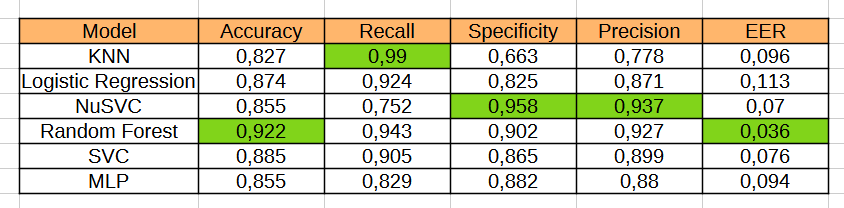
\includegraphics[width=0.8\textwidth]{Images/Results/Verification_single/st/VB_FA_BIG.png}
    \label{tab:VB_FA_BIG_st}
\end{table}

The Table \ref{tab:VB_FA_BIG_st} illustrates that the best-performing animation, in terms of accuracy, is VB\_FA\_BIG, achieving an accuracy of 92.2\% with the Random Forest classifier and an EER of 3.6\%.

\begin{table}[ht]
    \centering
    \caption{Verification results for single animations using the ST configuration and VB\_FA\_SMA animation.}
    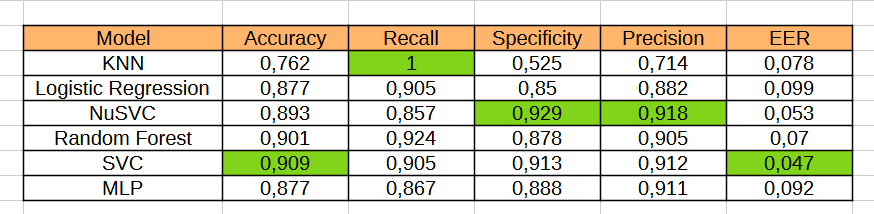
\includegraphics[width=0.8\textwidth]{Images/Results/Verification_single/st/VB_FA_LIT.png}
    \label{tab:VB_FA_LIT_st}
\end{table}


This animation is followed by VB\_FA\_SMA, which, as shown in Table \ref{tab:VB_FA_LIT_st}, achieves an accuracy of 90.9\% using the SVC classifier and an EER of 4.7\%.
The rest of the animation results are contained in Appendix \ref{subsec:vs_st_a}.

\begin{figure}[ht]
    \centering
    \includegraphics[width = 0.6
    \textwidth]{Images/Results/Verification_single/st/best_animation_roc_curves_st.png}
    \caption{ROC curves.}
    \label{fig:roc_st}
\end{figure}

The Figure \ref{fig:roc_st} presents the ROC curves for each individual animation, obtained using the best-performing classifier based on the Equal Error Rate.
For each curve and corresponding classifier, the Area Under the Curve (AUC) value is also reported in the legend as a performance indicator.
\FloatBarrier

\subsection{Verification single animation with intruders - Single Train (ST)}
\label{subsec:vsi}

After completing the closed-set verification analysis for the single animation and Single Train (ST) configuration, we proceed to perform the open-set analysis.
This analysis aims to evaluate how the system behaves when exposed to test data from users who were not included in the training phase.
In practical terms, this scenario simulates an unauthorized individual attempting to authenticate within a system where their identity is not previously registered.

As in the previous experiments, all classifiers are trained using the optimal hyperparameters identified during the identification phase, and the dataset is limited to the top k selected features to reduce computational load.
For this setup, the pool of 35 testers is divided into 24 enrolled users (representing authorized system members) and 11 intruders, approximately one-third of the total sample.
This division is governed by a fixed random seed to ensure the reproducibility of results across different runs.

For each of the 24 enrolled users, an individual model is trained using only the genuine data from that user for a single animation, considering samples from the first two sessions.
The training set is then balanced by adding an equal number of feature vectors randomly sampled from sessions 1 and 2 of other enrolled users.
This process is repeated 20 times with different random seeds, and the best-performing model is selected based on the highest training score.

Subsequently, 20 distinct test sets are generated, each containing the genuine user's data from session 3 along with an equal number of impostor samples randomly drawn from the intruder pool.
In this way, each test set includes both authorized and unauthorized data, effectively simulating real-world verification conditions.

Each of the 20 test sets is then used to evaluate the best-trained model, and the performance metrics are averaged to obtain a representative result for the corresponding user.
Finally, an overall performance estimate is computed by averaging the results across all 24 models, providing a general measure of system effectiveness under open-set verification conditions.

In this analysis, the accuracy of each animation generally decreases compared to the closed-set scenario, with the exception of VB\_SL\_SMA, which emerges as the best-performing animation.
This unexpected behavior may be attributed to the choice of evaluating all test sets using the globally best-performing model.
For this reason, an additional analysis employing the classic one-to-one training and testing approach will be conducted to enable a more direct comparison with the current results.
In principle, we would expect the best-performing animation to remain consistent between the open-set and closed-set verification analyses.
For VB\_SL\_SMA, accuracy increases from 85.9\% to 91.9\% when using the SVC classifier, while the EER decreases from 7.0\% to 6.1\%.
The corresponding results are illustrated in Table \ref{tab:VB_SL_LIT_sti}.

\begin{table}[ht]
    \centering
    \caption{Verification with intruders using the ST configuration and VB\_SL\_SMA animation.}
    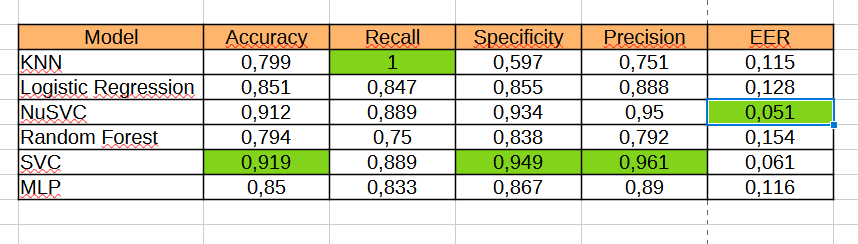
\includegraphics[width=0.8\textwidth]{Images/Results/Verification_single_intruders/st/VB_SL_LIT.png}
    \label{tab:VB_SL_LIT_sti}
\end{table}

The best-performing animation from the closed-set analysis, VB\_FA\_BIG, exhibits a decrease in accuracy from 92.2\% to 87.2\% when using the Random Forest classifier, while its EER increases from 3.6\% to 8.3\%.

\begin{table}[ht]
    \centering
    \caption{Verification with intruders using the ST configuration and VB\_FA\_BIG animation.}
    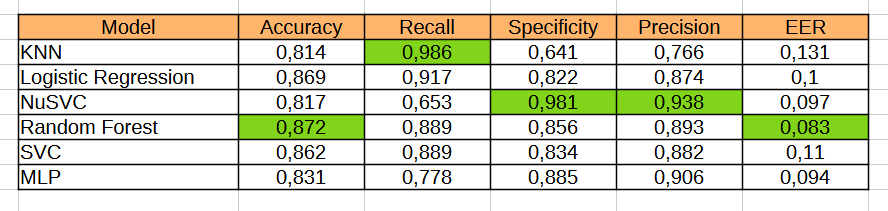
\includegraphics[width=0.8\textwidth]{Images/Results/Verification_single_intruders/st/VB_FA_BIG.png}
    \label{tab:VB_FA_BIG_sti}
\end{table}

Similarly, VB\_FA\_SMA, the second-best animation in terms of accuracy from the closed-set analysis, shows a slight decrease in accuracy from 90.9\% to 90.5\% when using the SVC classifier.
At the same time, its EER improves, decreasing from 4.7\% to 3.3\%.

\begin{table}[ht]
    \centering
    \caption{Verification with intruders using the ST configuration and VB\_FA\_SMA animation.}
    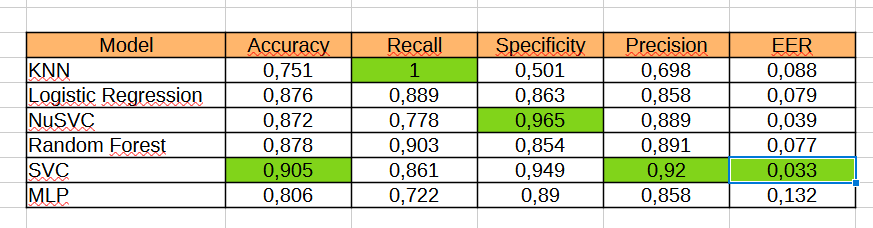
\includegraphics[width=0.8\textwidth]{Images/Results/Verification_single_intruders/st/VB_FA_LIT.png}
    \label{tab:VB_FA_LIT_sti}
\end{table}

All the remaining results are reported in Appendix \ref{subsec:vs_sti_a}.
To conclude the analysis, Figure \ref{fig:roc_sti} illustrates the ROC curves corresponding to each animation, generated using the classifier that achieved the lowest EER.


\begin{figure}[ht]
    \centering
    \includegraphics[width = 0.6
    \textwidth]{Images/Results/Verification_single_intruders/st/best_animation_roc_curves_st.png}
    \caption{ROC curves.}
    \label{fig:roc_sti}
\end{figure}
\FloatBarrier

\subsection{Verification Single Animation with Reduced Session Duration - Single Train (ST)}

The goal of the following section is to extend the single-animation verification using the Single Train (ST) configuration in order to evaluate the performance of the best animation when the recording duration is reduced.
In particular, the same program described in Section \ref{subsec:vs_st} is executed, with the only modification being the dataset composition.
In this case, the datasets consist of data recorded during the first ten seconds and first five seconds from the start of each animation.
The GP3\_HD eye tracker operates at a sampling rate of 150 Hz, meaning that 150 data points are collected per second and stored as rows in the output CSV file.
Accordingly, the dataset for the 10-second variation includes the first 1,500 samples (150 x 10) of each recording, while the 5-second variation contains the first 750 samples (150 x 5).

This analysis is particularly important, as it aims to evaluate how the performance of the best animation changes when the recording duration is reduced.
The objective is to identify an optimal trade-off between accuracy and acquisition time, a factor that will be crucial in real-world applications.
In practice, if the animation duration is too long, users may lose focus or abandon the procedure, negatively affecting both data quality and system usability.

\begin{table}[ht]
    \centering
    \caption{Verification results with 10-second recordings using the ST configuration and VB\_FA\_BIG animation.}
    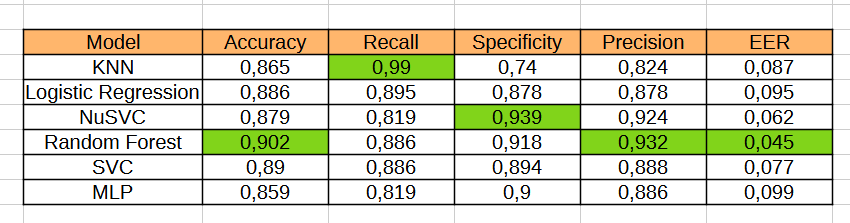
\includegraphics[width=0.8\textwidth]{Images/Results/Verification_single_five_ten/st/ten/VB_FA_BIG.png}
    \label{tab:VB_FA_BIG_10_st}
\end{table}

\begin{table}[ht]
    \centering
    \caption{Verification results with 5-second recordings using the ST configuration and VB\_FA\_BIG animation.}
    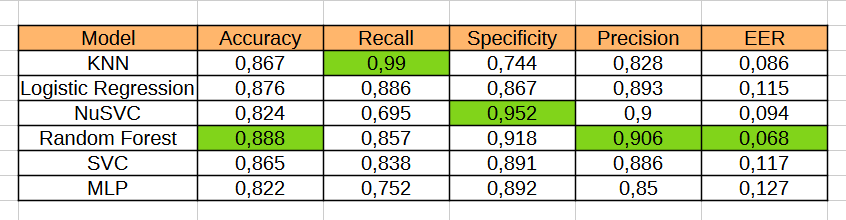
\includegraphics[width=0.8\textwidth]{Images/Results/Verification_single_five_ten/st/five/VB_FA_BIG.png}
    \label{tab:VB_FA_BIG_5_st}
\end{table}


As expected, the best-performing animation remains VB\_FA\_BIG, consistent with the results obtained in the 15-second analysis.
When considering only the first 10 seconds, its accuracy decreases slightly from 92.2\% to 90.2\% using the Random Forest classifier, while the EER increases from 3.6\% to 4.5\%.
When the duration is further reduced to 5 seconds, accuracy drops to 88.8\%, and the EER rises to 6.8\%.

These results are highly encouraging, as they demonstrate that the model maintains strong performance even with significantly shorter recording times.
With a 10-second window, accuracy remains around 90\%, indicating minimal degradation, while the 5-second configuration still achieves a notably high accuracy of 88.8\%.
Depending on the intended application and operational constraints, any of these configurations may be selected to balance efficiency and reliability according to specific requirements.

We are interested only in the results obtained with the best-performing animation.
The remaining results for the other animations are presented in Appendix \ref{subsec:vs_st_ft}, due to space constraints.

\begin{figure}[ht]
    \centering
    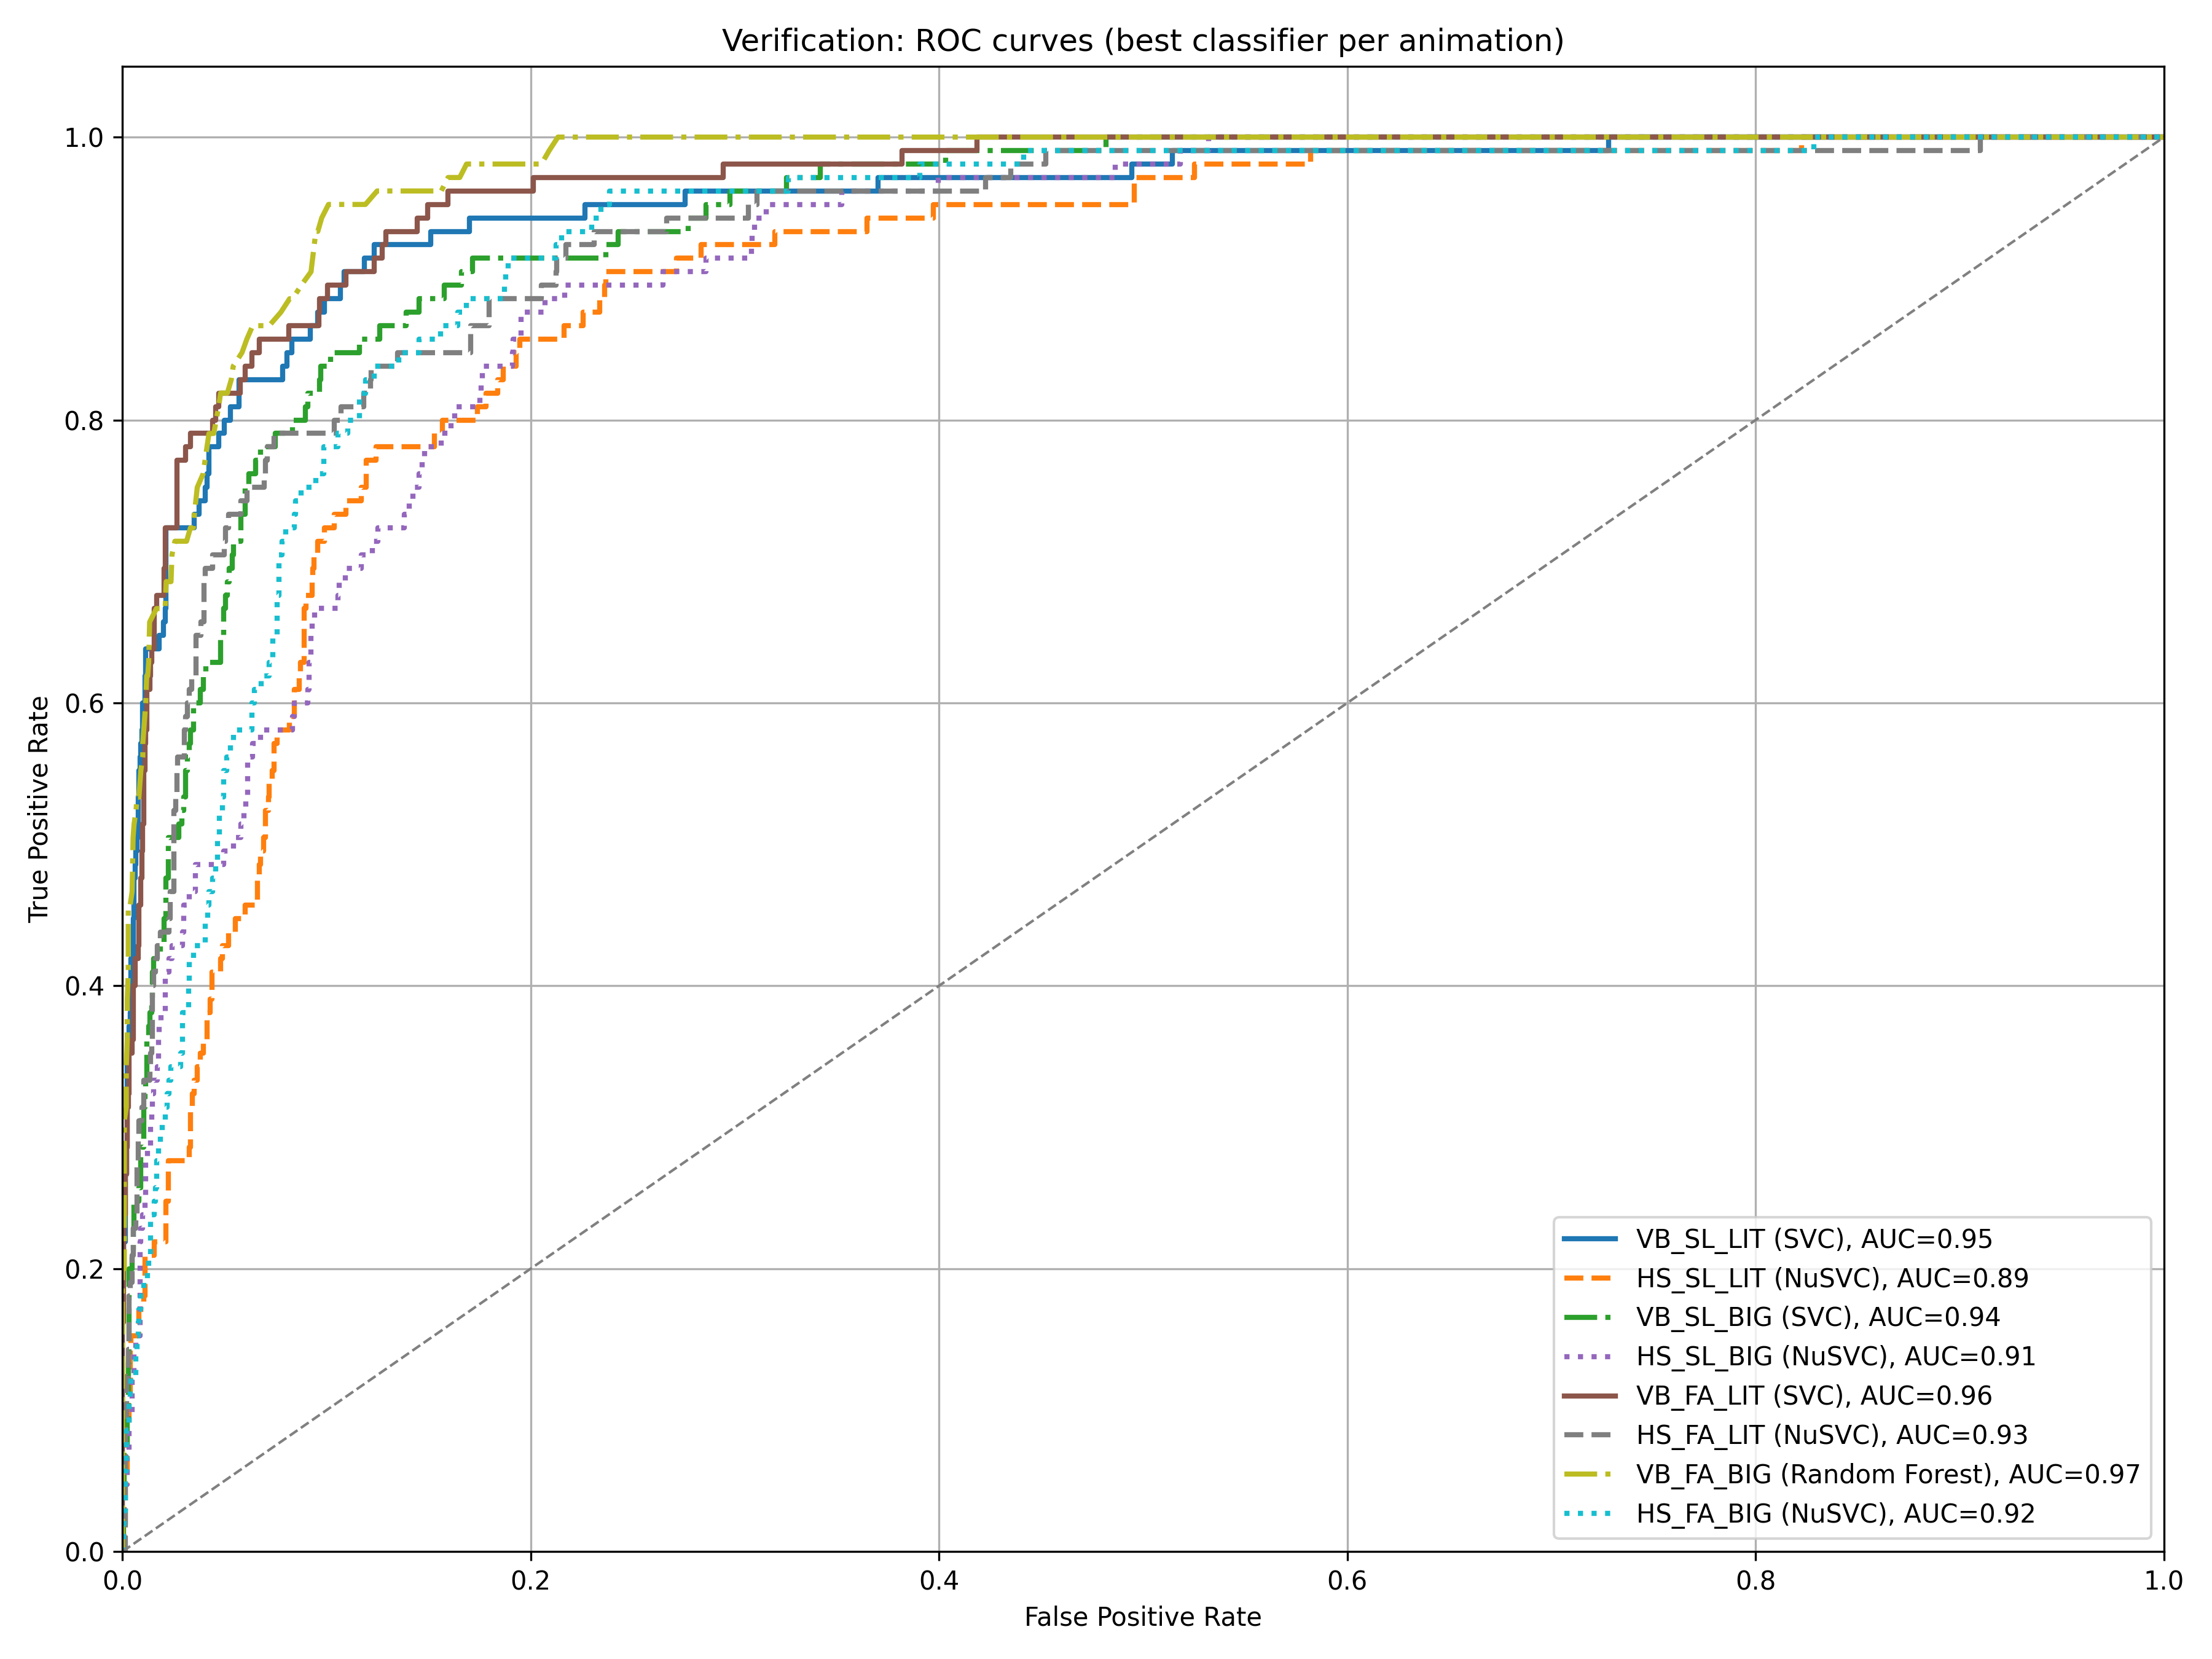
\includegraphics[width = 0.6
    \textwidth]{Images/Results/Verification_single_five_ten/st/ten/best_animation_roc_curves_ten_st.png}
    \caption{ROC curves 10 seconds.}
    \label{fig:roc_t}
\end{figure}

\begin{figure}[ht]
    \centering
    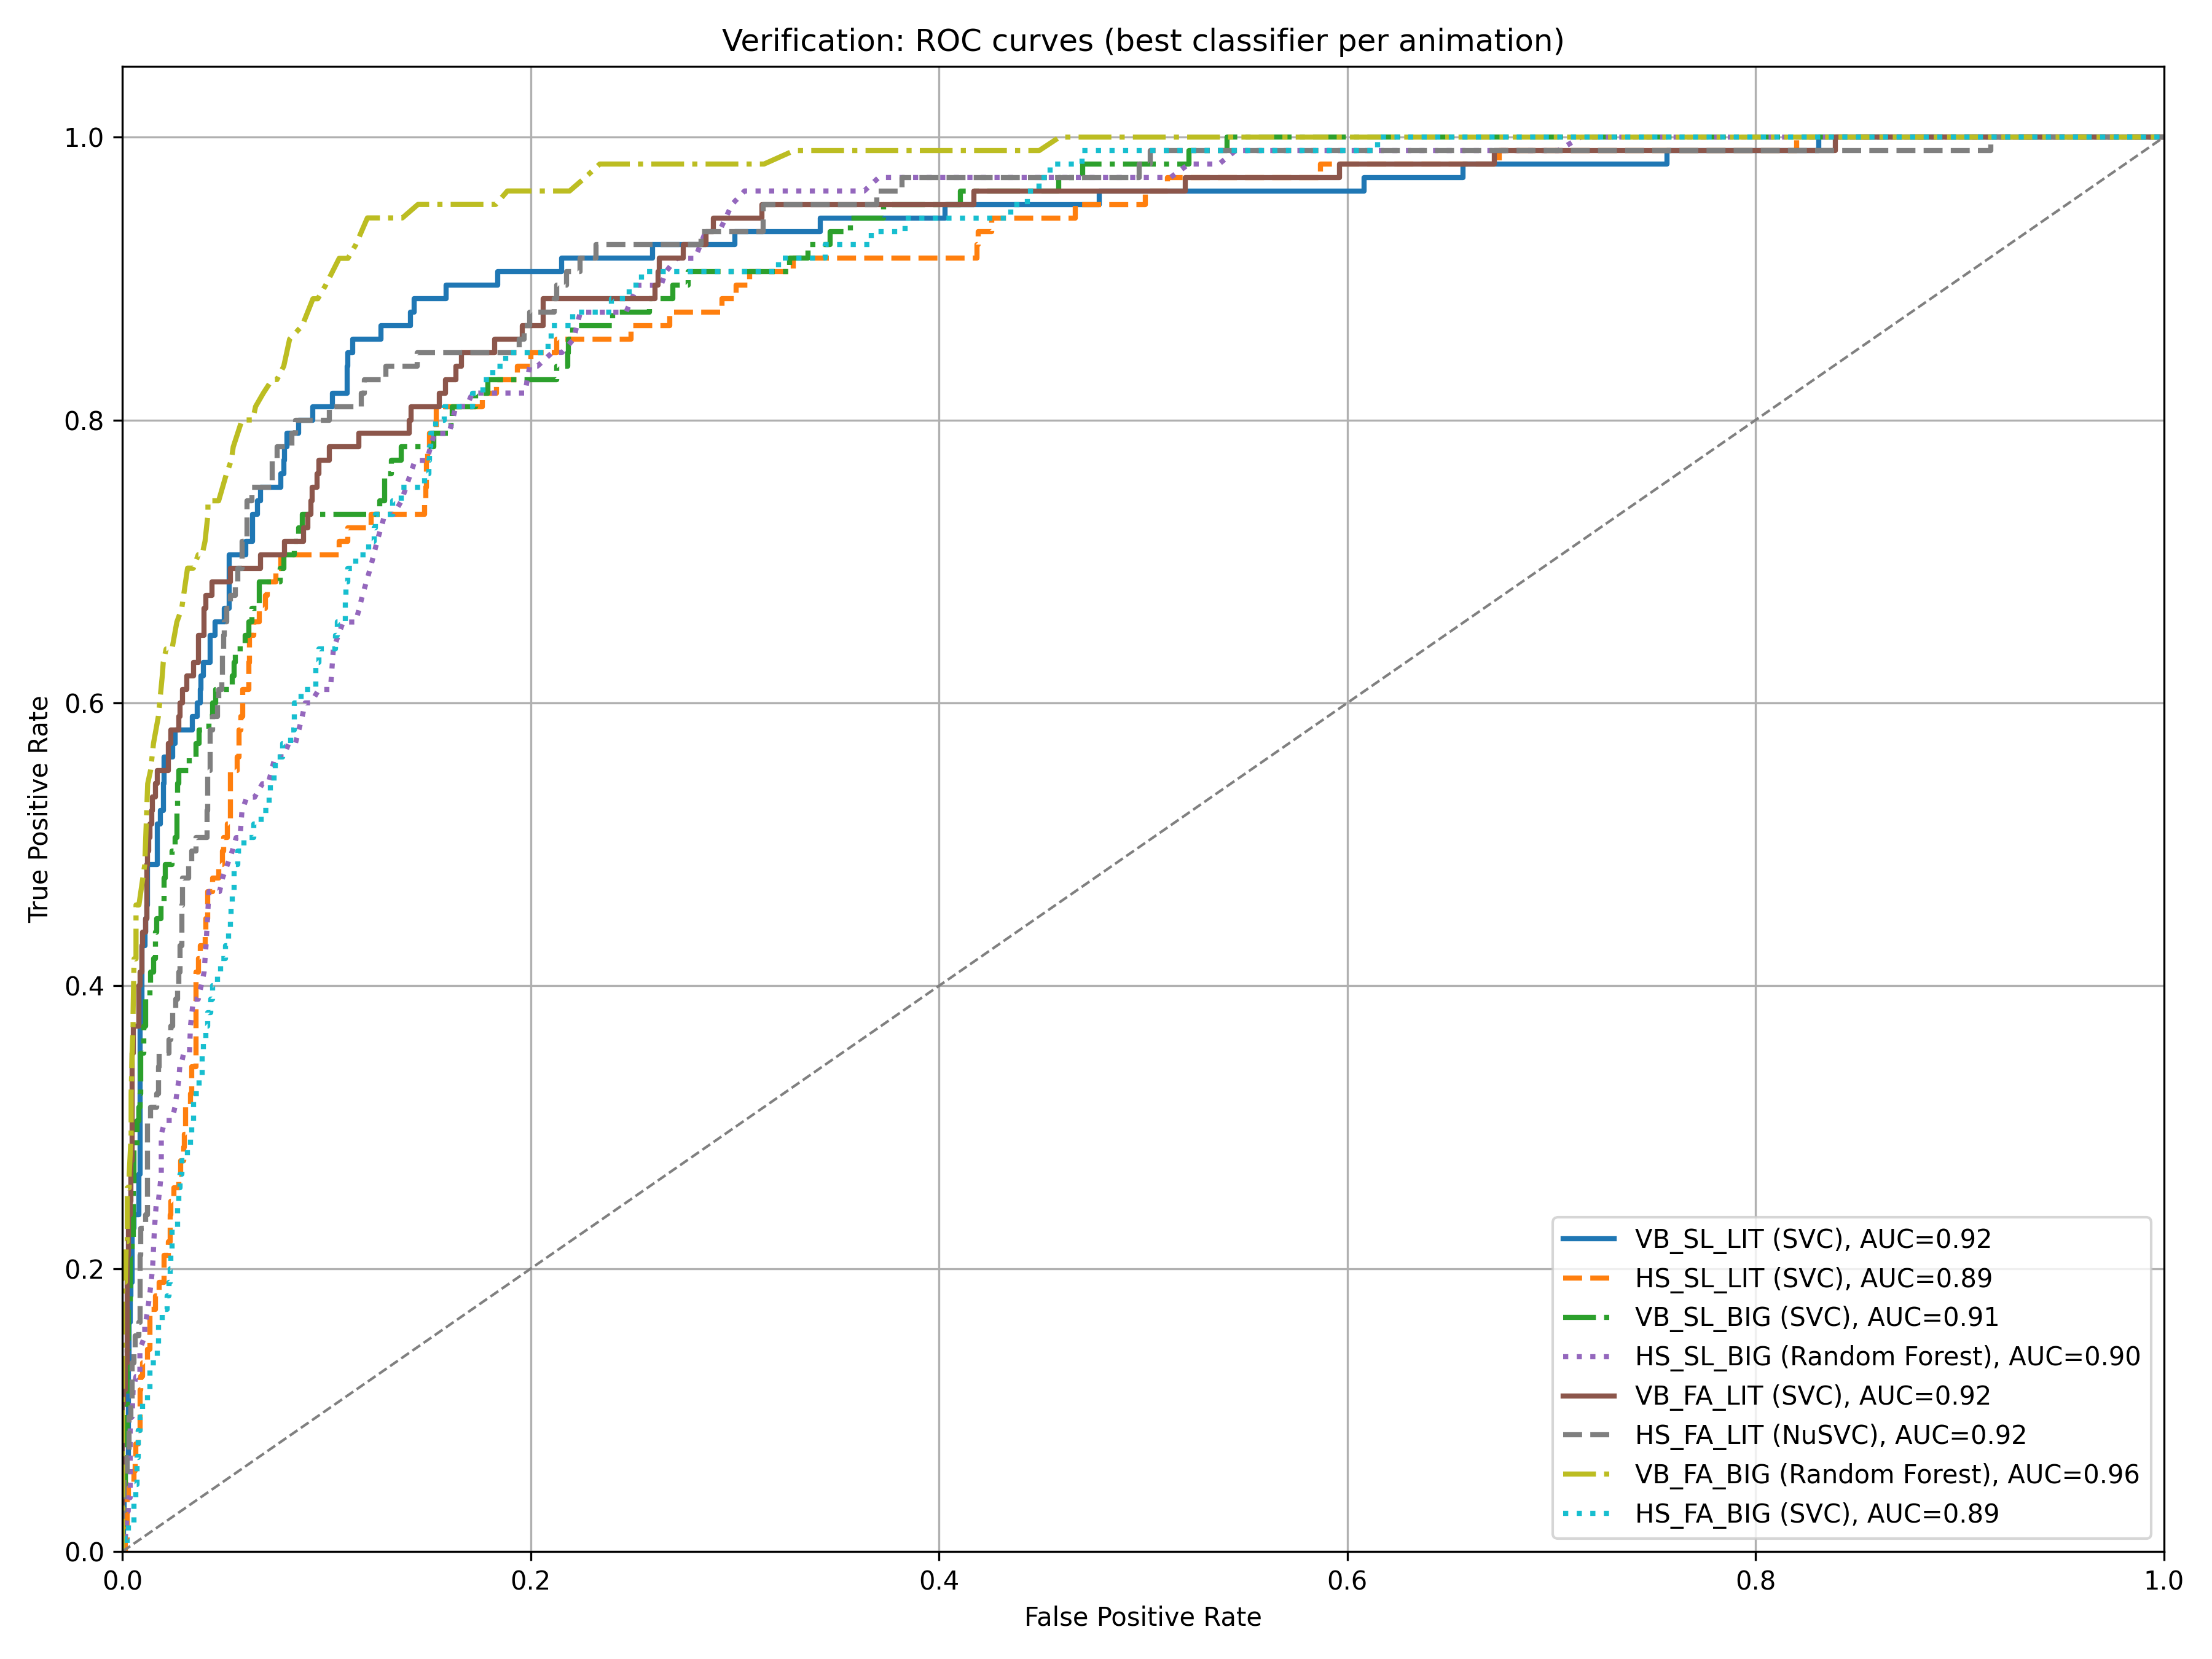
\includegraphics[width = 0.6
    \textwidth]{Images/Results/Verification_single_five_ten/st/five/best_animation_roc_curves_five_st.png}
    \caption{ROC curves 5 seconds.}
    \label{fig:roc_f}
\end{figure}

To conclude this section, we present the two ROC curves based on the EER obtained from both analyses.
Specifically, Figures \ref{fig:roc_t} and \ref{fig:roc_f} correspond respectively to the 10-second and 5-second analyses.
\FloatBarrier

\section{Verification 'classic' single animation - ST type}

The following section presents the same analysis described in Section \ref{subsec:prima_ver}, with a minor modification in the evaluation procedure.

In the previous section, twenty models were trained for each individual, with each model corresponding to a distinct random seed.
Among these twenty training configurations, only the model achieving the highest training accuracy was selected as the best-performing instance.
Using the same twenty random seeds, an equivalent number of independent test sets were subsequently generated.
These test sets were employed exclusively for the evaluation of the selected best model, ensuring that all testing procedures were conducted on the same trained model.
In contrast, the current procedure differs in that twenty separate models are both trained and evaluated, one for each random seed.

The rationale behind the previous approach, evaluating all configurations using the single best model, was to explore whether such a strategy could yield superior results.
To provide a meaningful comparison, the results of this more conventional verification analysis are also included.

\subsection{Verification single animation classic without intruders - single train(ST)}
\label{subsec:s_vs_cst}

This and the following sections present the classic verification analysis performed on single animations.
The term classic refers to the fact that, instead of evaluating only the best-performing model based on training accuracy, each model is trained and tested as a pair for every individual seed.
As before, two levels of averaging are computed: one across all repetitions for each participant, and another across participants for each classifier.

This analysis is therefore a direct mirror of the previous one, still employing the Single Train (ST) configuration.
For this reason, the methodological details will not be repeated here.
Instead, we will focus on presenting the results and comparing them to identify the most consistent and effective approach.

As in the previous analysis, the best-performing animation remains VB\_FA\_BIG, achieving an accuracy of 92.4\% using the NuSVC classifier and an EER of 4.6\%.
When comparing the two analyses, the results are almost identical, with this configuration showing a slight improvement of 0.2\% in accuracy, but a small increase in EER from 3.6\% to 4.6\%.

\begin{table}[ht]
    \centering
    \caption{‘Classic’ verification results using the ST configuration and VB\_FA\_BIG animation.}
    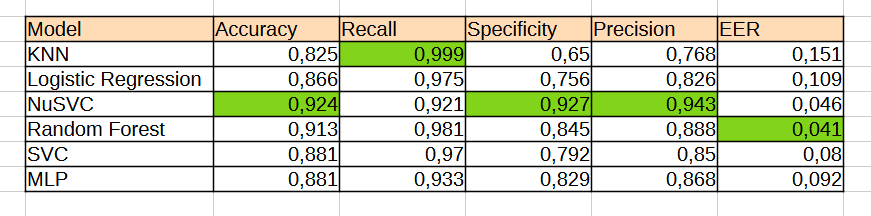
\includegraphics[width=0.8\textwidth]{Images/Results/Classic_procedure/Verification_single/st/VB_FA_BIG.png}
    \label{tab:VB_FA_BIG_cst}
\end{table}

The Table \ref{tab:VB_FA_BIG_cst} display the best performing animation, while the additional results regarding the other animations are contained in Appendix \ref{subsec:vsc_st_ft}.

As in the previous chapter, this analysis includes the ROC curves for the best-performing animations, selected based on their EER, as shown in Figure \ref{fig:roc_cst}.

\begin{figure}[ht]
    \centering
    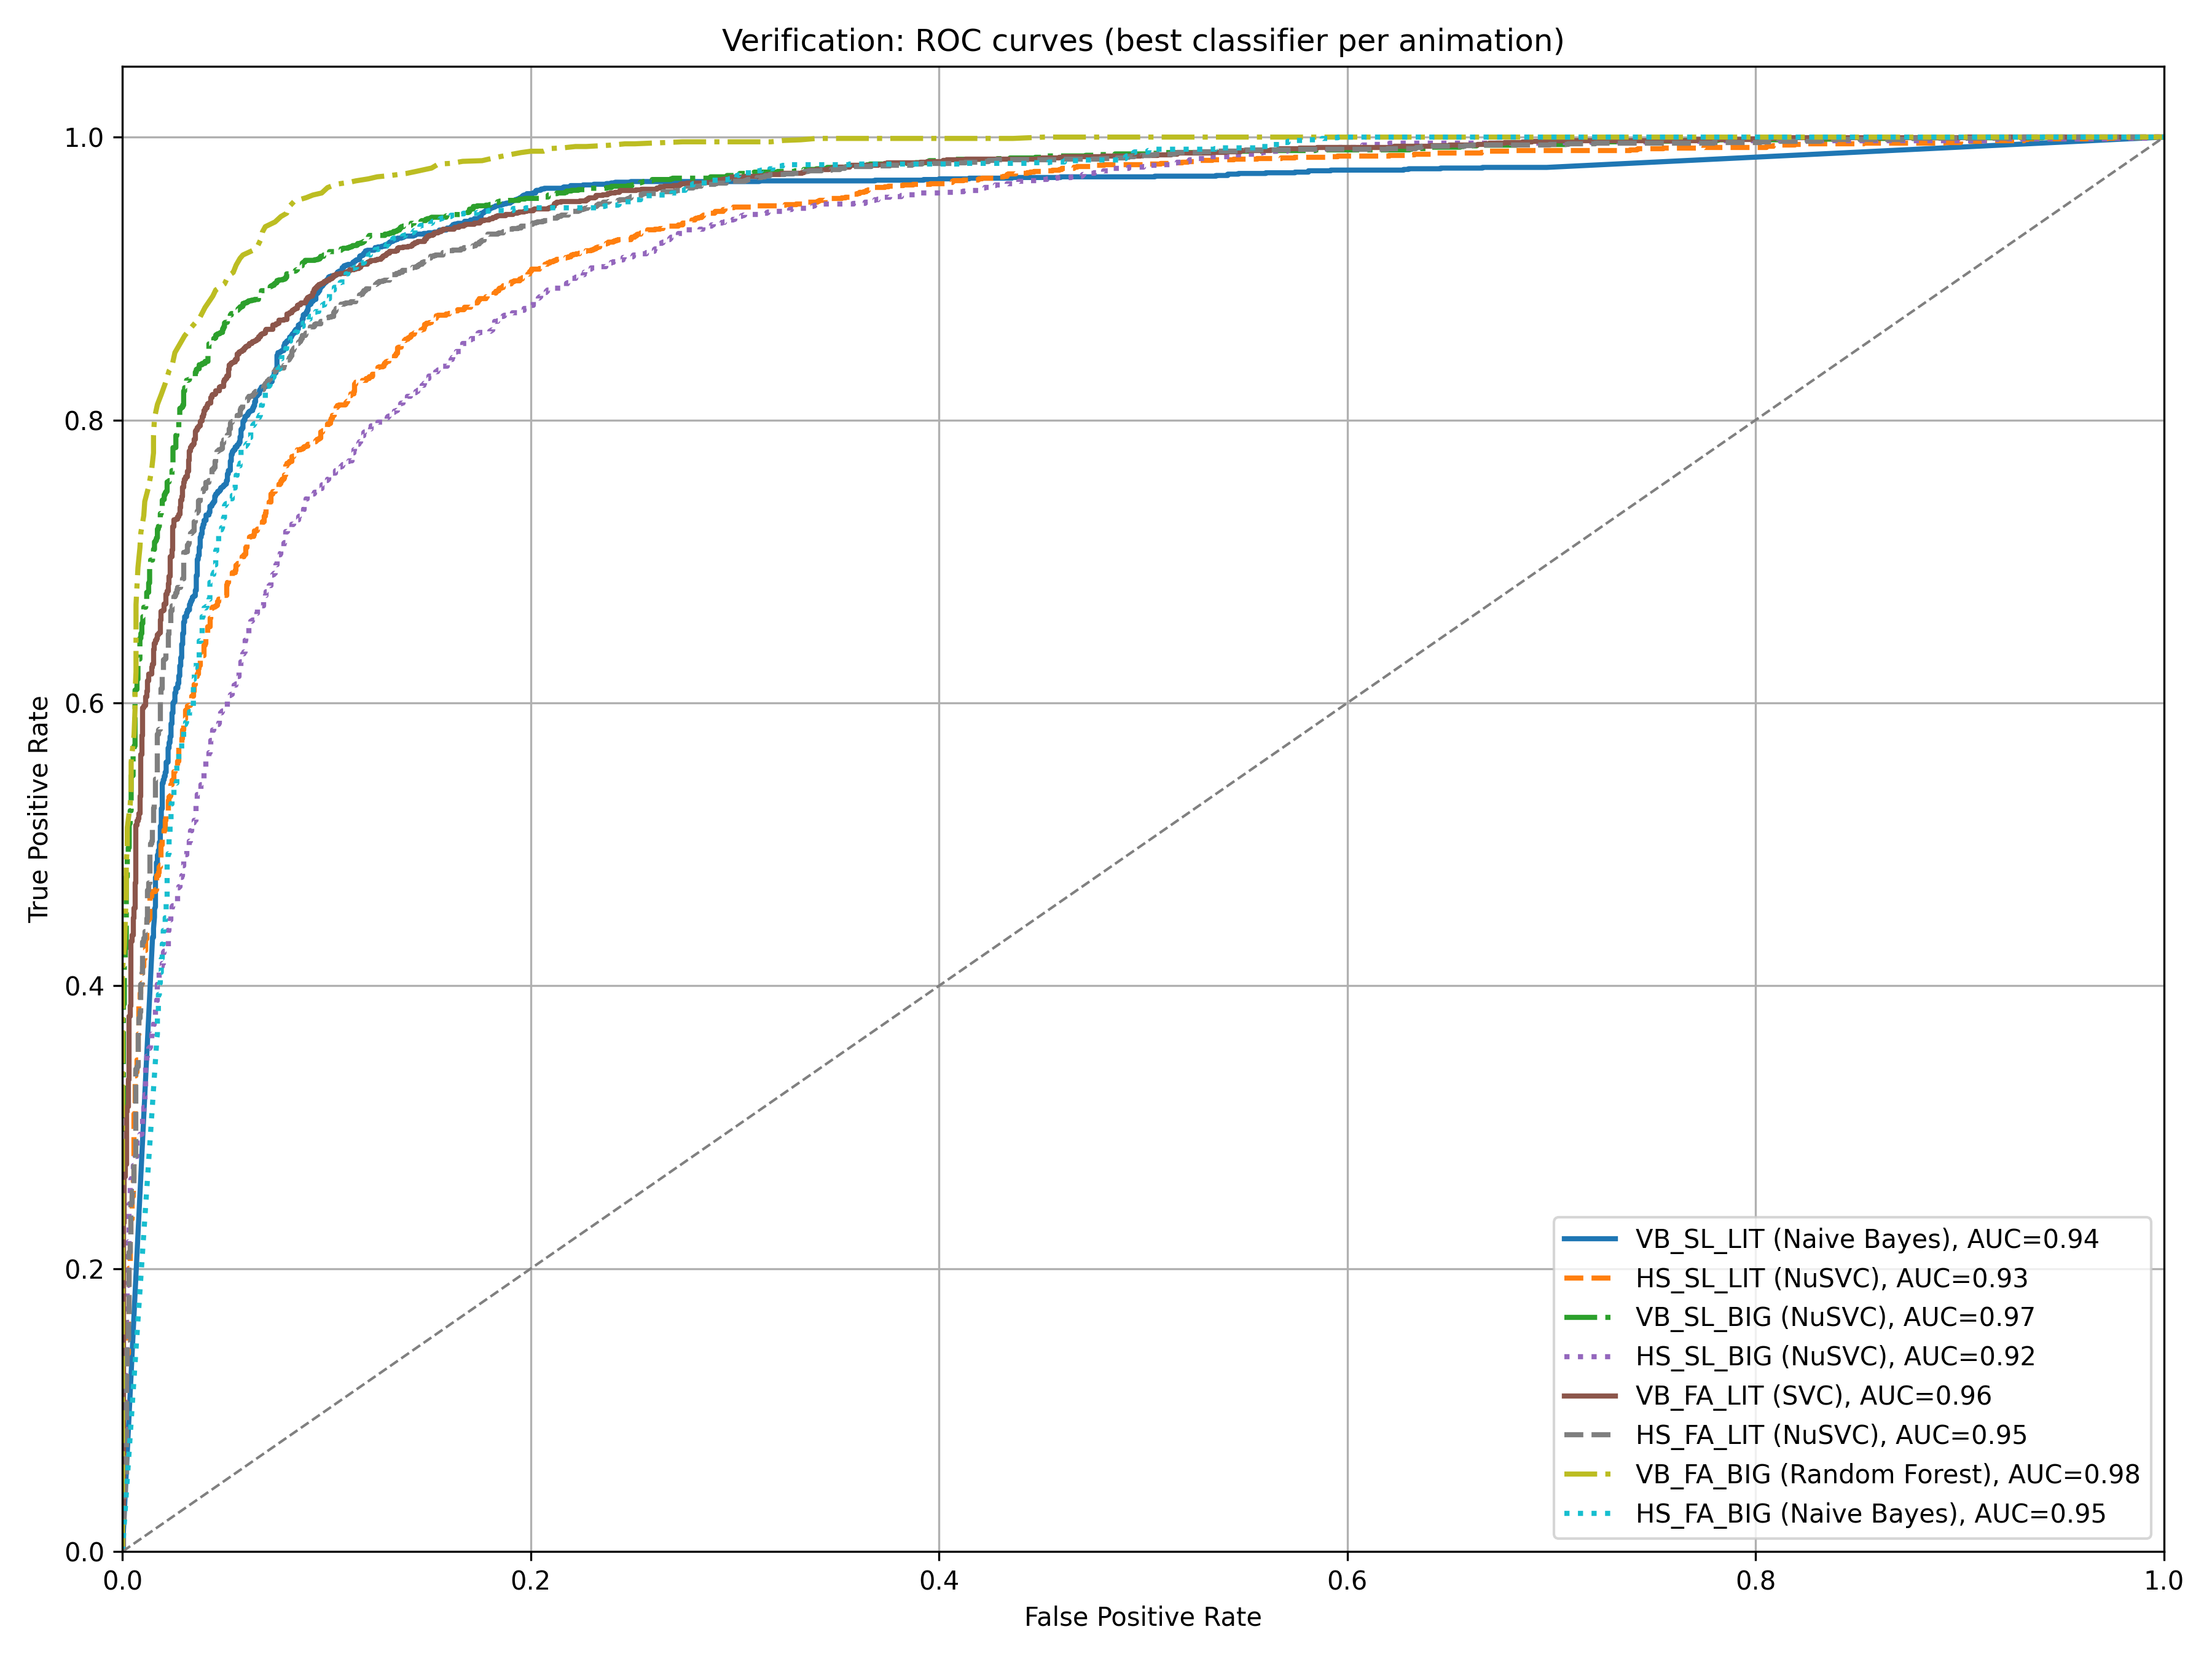
\includegraphics[width = 0.6
    \textwidth]{Images/Results/Classic_procedure/Verification_single/st/Verification_single_roc_classic_st.png}
    \caption{ROC curves.}
    \label{fig:roc_cst}
\end{figure}
\FloatBarrier


\subsection{Verification 'classic' single animation with intruders - Single Train(ST)}

To proceed, we performed the analysis with unseen users in the test set, referred to as intruders.
Following the closed-set analysis, this intruder-based evaluation was carried out in the same way as in the previous section, with only minor updates to the evaluation procedure.

The first observation from these results is that the best-performing animation remains consistent with the previous section, regarding the closed set analysis.
This continuity is particularly important, as it suggests that the anomalous behavior observed earlier was likely due to the evaluation procedure rather than inherent differences in the data or model performance.

\begin{table}[ht]
    \centering
    \caption{‘Classic’ verification with intruders using the ST configuration and VB\_FA\_BIG animation.}
    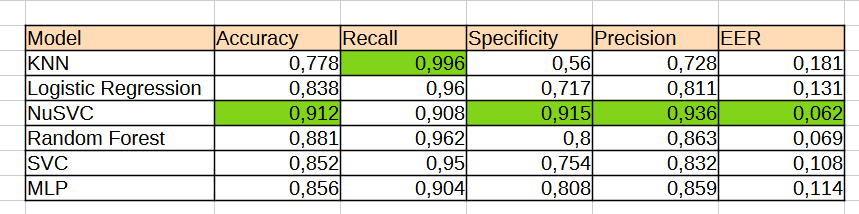
\includegraphics[width=0.8\textwidth]{Images/Results/Classic_procedure/Verification_intruders/st/VB_FA_BIG.png}
    \label{tab:VB_FA_BIG_cist}
\end{table}


As we observe from Table \ref{tab:VB_FA_BIG_cist} we have a decrease in accuracy from 92.4\% to 91.2\% using nuSVC classifier and an increase of the EER from 4.6\% to 6.2\%.
This behavior is expected due to the presence of unseen users in the dataset.
However, the performance decrease remains relatively small, indicating that the system continues to perform effectively even under this more challenging evaluation scenario.

When comparing these results with the analysis performed using the best model for evaluation, we observe comparable performance: 91.2\% with nuSVC versus 91.9\% obtained with SVC. 
The equal error rate is also nearly identical, with 6.2\% in the current analysis compared to 6.1\% previously. 
However, we consider the current results preferable for everyday applications, as they offer continuity in performance with the same animation. 
In practical scenarios, it is advantageous to maintain a single animation that performs optimally in both closed-set and open-set conditions.

\begin{figure}[ht]
    \centering
    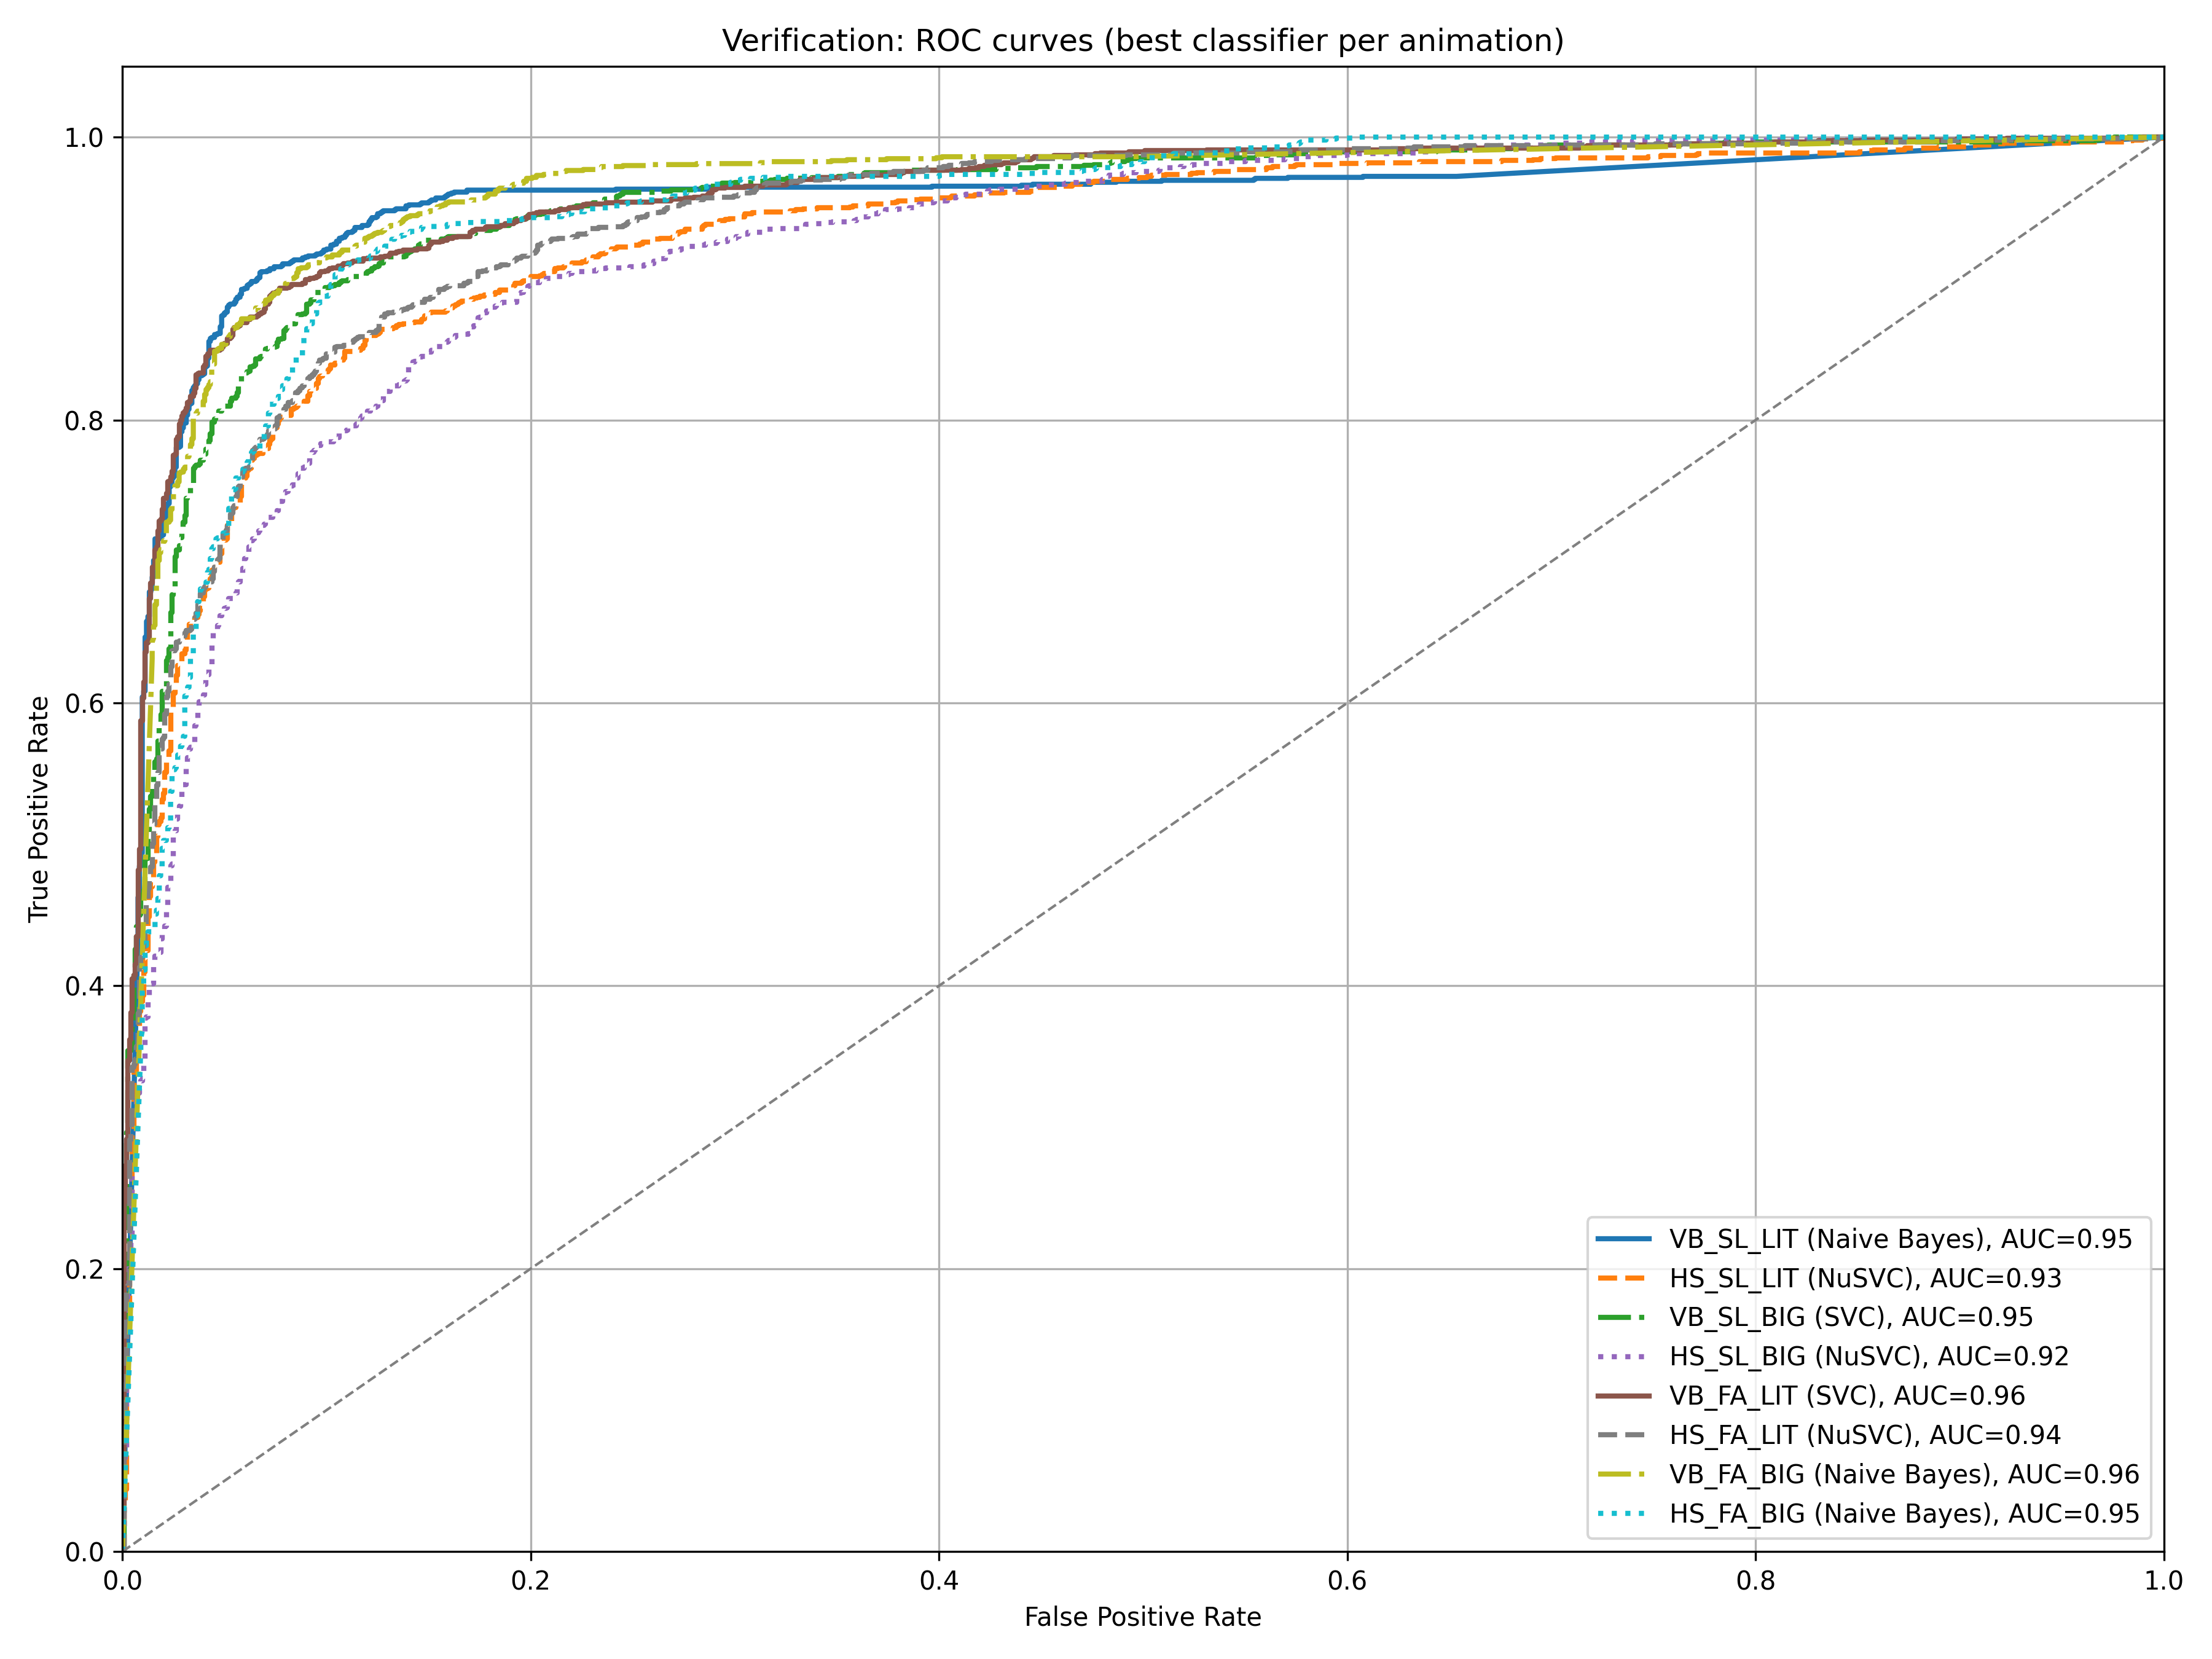
\includegraphics[width = 0.6
    \textwidth]{Images/Results/Classic_procedure/Verification_intruders/st/Verification_single_intruders_roc_two_st.png}
    \caption{ROC curves.}
    \label{fig:roc_cist}
\end{figure}

To maintain consistency with the previous analyses, the ROC curve based on the Equal Error Rate is presented in Figure \ref{fig:roc_cist}. 
Additional results related to this analysis are provided in the corresponding appendix (Appendix \ref{subsec:vsci_st_ft}).
\FloatBarrier

\subsection{Verification 'classic' Single Animation with Reduced Session Duration - Single Train (ST)}

We conclude this analysis in the same manner as in the previous subsection, by conducting a reduced animation time evaluation. 
Specifically, we examine how the results change when reducing the total duration from 15 seconds to 10 seconds, and then to 5 seconds.

The results remain consistent with our expectations, with VB\_FA\_BIG maintaining its position as the best-performing animation based on the accuracy score. 
Notably, its performance declines only slightly, from 92.4\% to 91.5\% using nuSVC, when the recording time is reduced to 10 seconds. 
Concurrently, its EER increases modestly from 4.6\% to 5.3\%.

If recordings are limited to only the first 5 seconds of data, performance further decreases to 90.8\%, and the EER rises to 8\%. 
These findings indicate a trade-off between recording duration and system performance, with relatively minor degradation for shorter recordings.

The best-performing animation resulst are collected in Tables \ref{tab:VB_FA_BIG_cst_10} and \ref{tab:VB_FA_BIG_cst_5}.
While the ROC  curves of this analysis are presented in figures \ref{fig:roc_cst_10} and \ref{fig:roc_cst_5}.
All the additional material related to this type of analysis is placed in Appendix \ref{subsec:vsc_rt}.

\begin{table}[ht]
    \centering
    \caption{Verification ’classic’ results with 10-second recordings using the ST configuration and VB\_FA\_BIG animation.}
    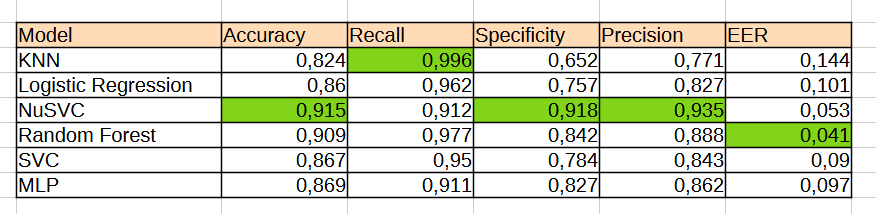
\includegraphics[width=0.8\textwidth]{Images/Results/Classic_procedure/five_ten/st/ten/VB_FA_BIG.png}
    \label{tab:VB_FA_BIG_cst_10}
\end{table}

\begin{table}[ht]
    \centering
    \caption{Verification ’classic’ results with 5-second recordings using the ST configuration and VB\_FA\_BIG animation.}
    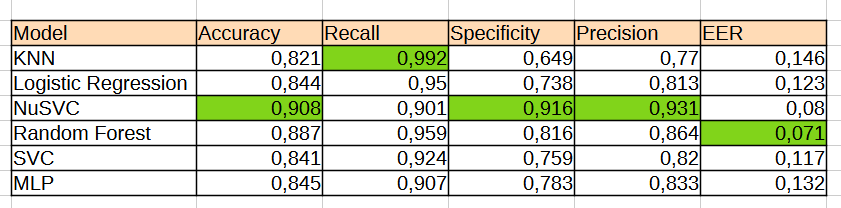
\includegraphics[width=0.8\textwidth]{Images/Results/Classic_procedure/five_ten/st/five/VB_FA_BIG.png}
    \label{tab:VB_FA_BIG_cst_5}
\end{table}


\begin{figure}[ht]
    \centering
    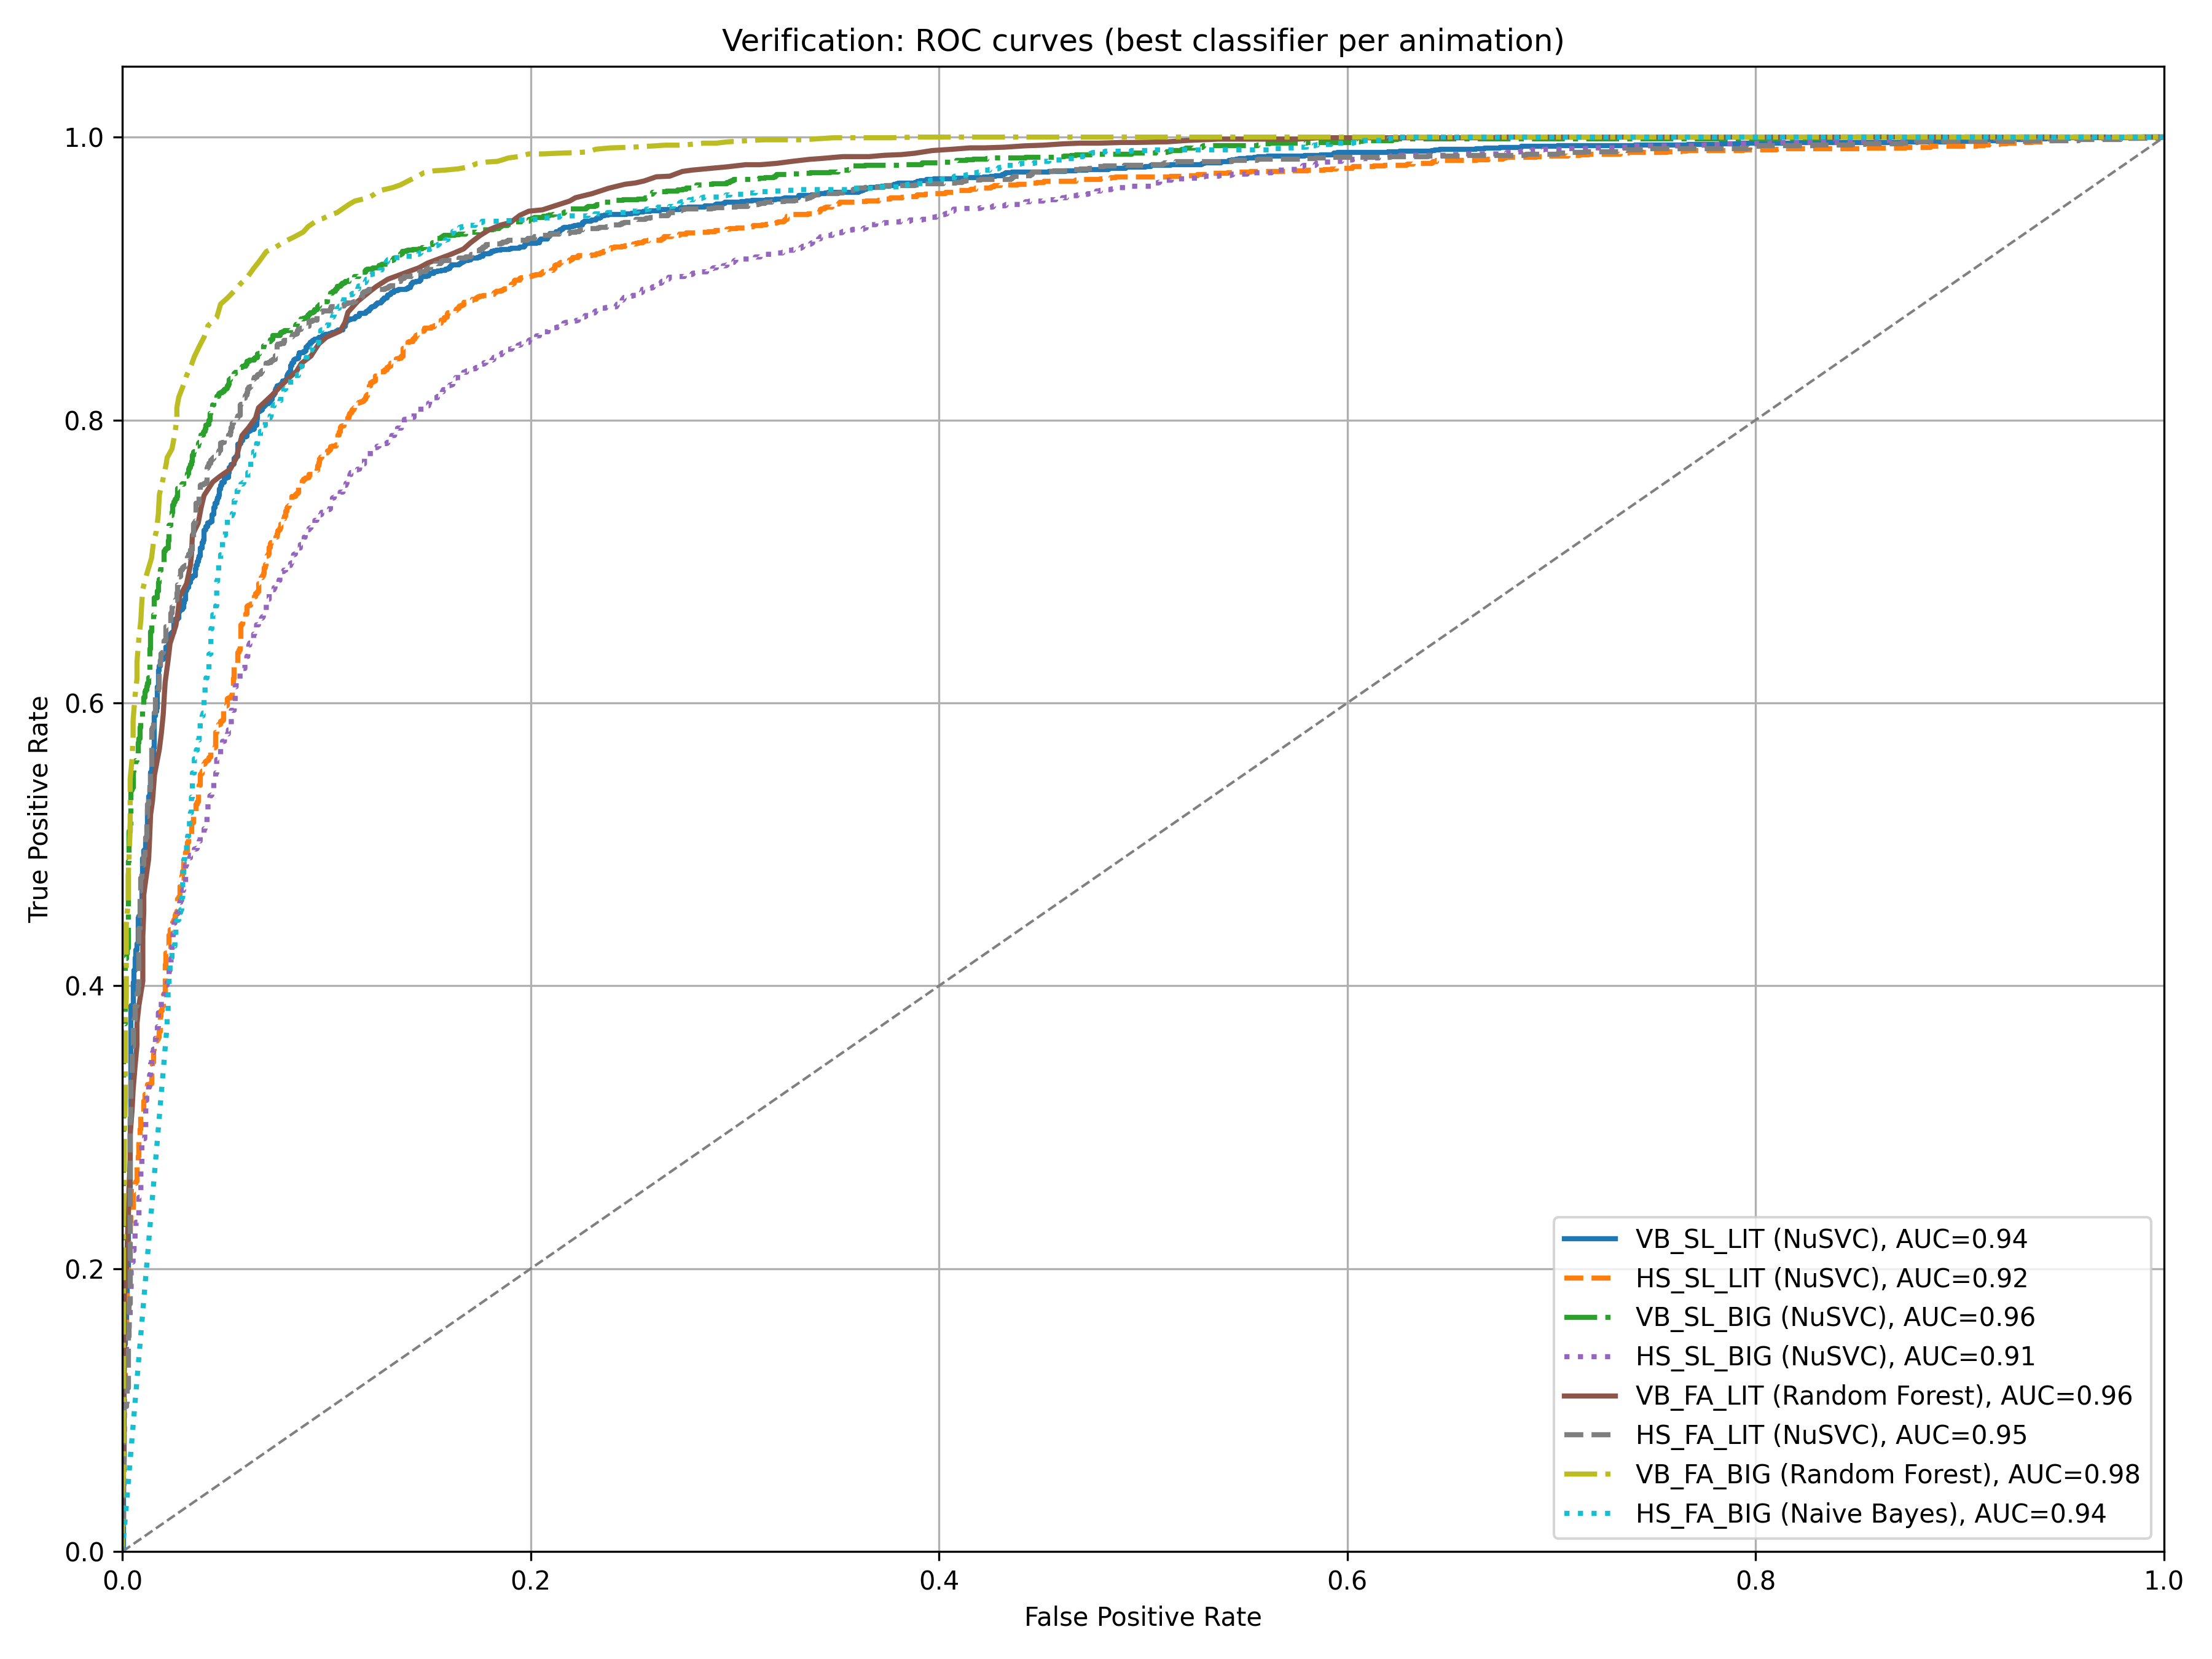
\includegraphics[width = 0.6
    \textwidth]{Images/Results/Classic_procedure/five_ten/st/ten/Verification_single_roc_classic_ten_st.png}
    \caption{ROC curves - 10 seconds.}
    \label{fig:roc_cst_10}
\end{figure}

\begin{figure}[ht]
    \centering
    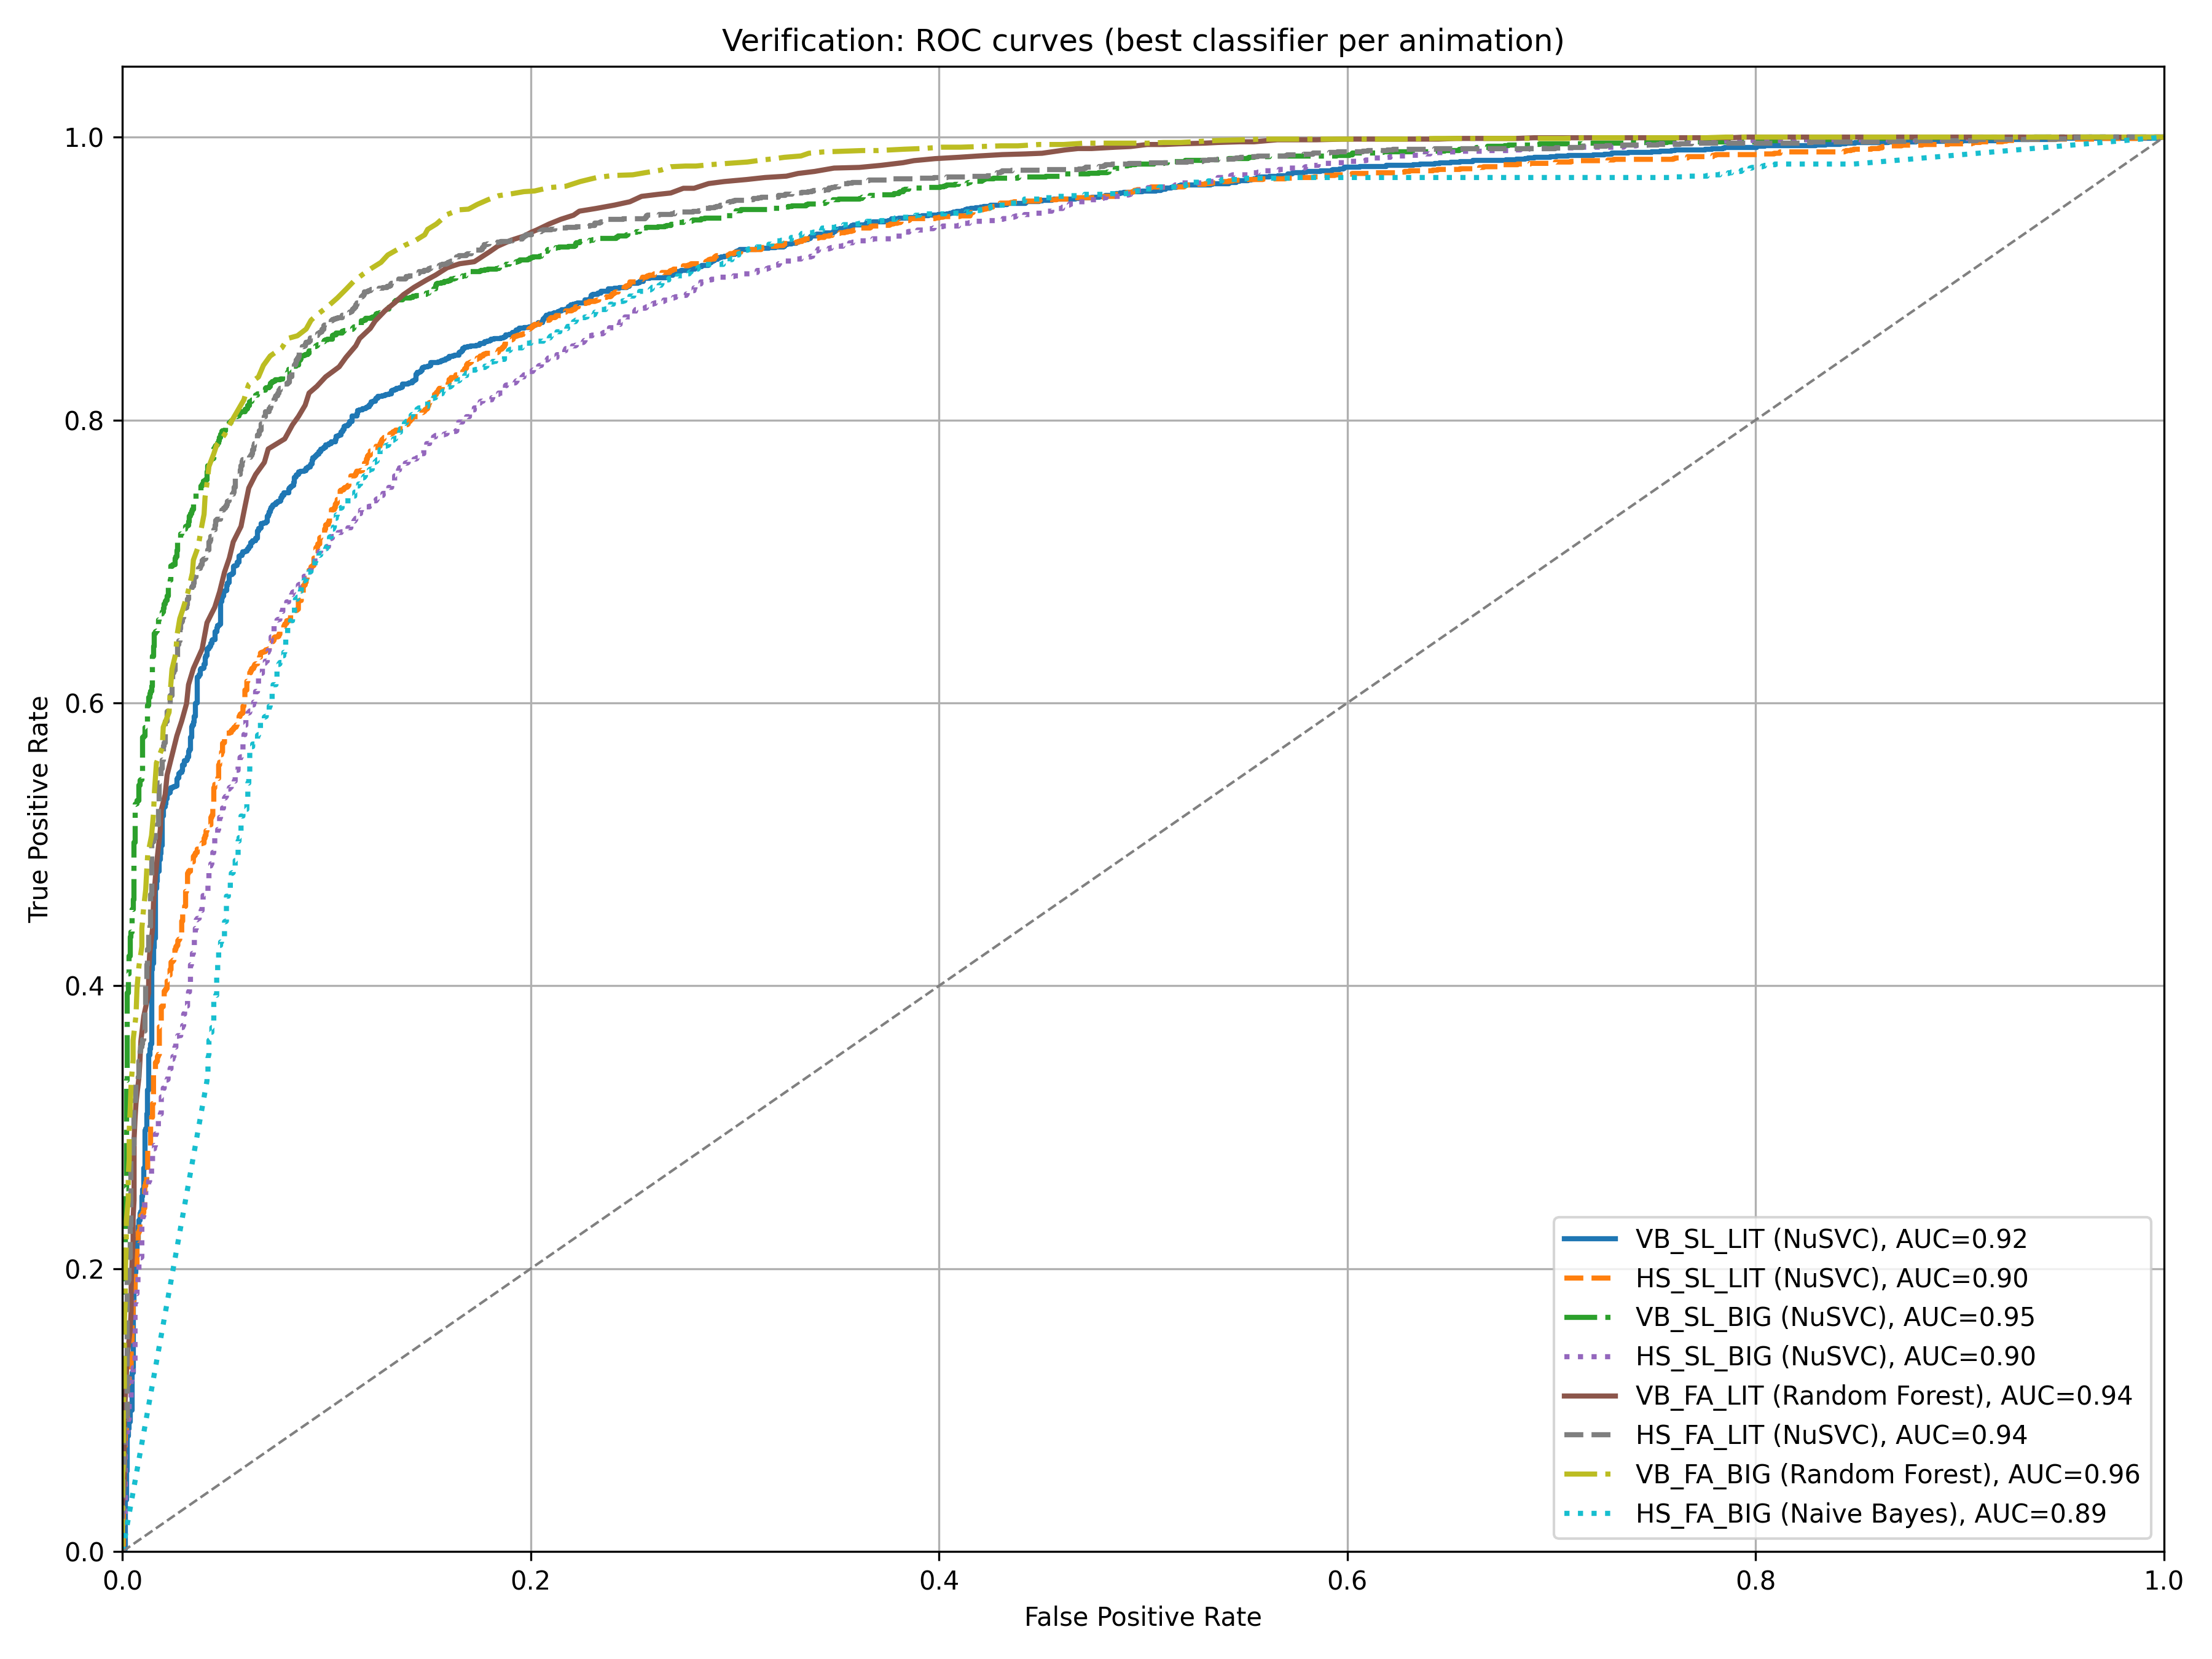
\includegraphics[width = 0.6
    \textwidth]{Images/Results/Classic_procedure/five_ten/st/five/Verification_single_roc_classic_five_st.png}
    \caption{ROC curves - 5 seconds}
    \label{fig:roc_cst_5}
\end{figure}

To conclude this section, we compare the results obtained in the current analysis with those from the previous section, conducted under the same reduced time conditions.
When considering the ten-second recordings, the current procedure slightly outperforms the previous one, achieving an accuracy of 91.5\% with SVC compared to 90.2\% obtained using Random Forest. 
The equal error rate also improves, decreasing from 4.5\% to 4.1\%.
For the five-second recordings, the trend remains similar: the current analysis reaches a higher accuracy of 90.8\% with nuSVC, compared to 88.8\% achieved with Random Forest in the previous analysis. 
However, this improvement in accuracy comes at the cost of a higher equal error rate, which increases from 6.8\% to 8\%.

In conclusion, this evaluation generally outperforms the previous approach, with the exception of the slight increase in EER for the shortest animation duration.
The choice between the two methods should ultimately depend on the specific application requirements. 
In particular, if time constraints are not critical, or if recordings of up to ten seconds are feasible, the current analysis is preferred. 
Conversely, for five-second recordings, the preferred method depends on whether the application favours accuracy or robustness against errors.
\FloatBarrier

\section{Verification single animation - FT}
\label{subsec:terza_ver}

We now move to the third part of the verification analysis.
In this case, we adopt a procedure similar to the one previously described, with the main difference being that all animations are used for training, while testing is still performed on single animations.
The objective is to evaluate whether increasing the amount of training data can lead to improved model performance.
The following analysis serves as the counterpart to the experiment described in Section \ref{subsec:prima_ver}. 
Its purpose is to provide a direct and systematic comparison between the two methodologies, allowing for a clearer evaluation of their respective performance and consistency.

\subsection{Verification single animation without intruders - Full Train(FT)}
\label{subsec:vft}

As previously stated, the main objective of this work is to identify the animation that achieves the best verification performance. 
For this reason, the evaluation continues to focus on the single-animation configuration. 
Only the session-based data split is employed in this phase, as it most accurately reflects realistic application scenarios.

In this analysis, each model is trained using the same classifiers described in Appendix \ref{subsec:param}, employing only their optimal parameter configurations. 
Specifically, the training process utilizes the top-ranked features extracted through the SelectKBest method and the best hyperparameters identified during the corresponding identification analysis through GridSearchCV.

This section presents the Full Train (FT) configuration, which represents a closed-set verification scenario. 
In this setting, all subjects included in the evaluation phase are also present in the training phase, and therefore no testing is performed on previously unseen individuals.
As in the other verification analyses, a dedicated model is trained for each individual subject. 
The Full Train (FT) configuration introduces a key difference compared to the Single Train (ST) approach. 
In this configuration all data from each subject are used for training, including every animation from sessions S1 and S2 instead of limiting the process to a single animation.
To ensure class balance, an equivalent amount of impostor data is randomly sampled from the S1 and S2 data of other subjects.
The test set, on the other hand, consists exclusively of data from a single animation of the target subject in session S3. 
It is complemented by an equal number of randomly selected impostor samples taken from other users' S3 data.

Each model is then trained and evaluated on its corresponding paired train-test sets.
This entire procedure is repeated across twenty different random seeds to mitigate the influence of stochastic variability and to ensure that the reported results are statistically robust. 
Consequently, each user-specific model is trained and evaluated twenty times, and the individual results are averaged to obtain the user's mean performance. 
Finally, an additional averaging step across all users is performed to derive the overall system performance.

The evaluation of the models is not limited to classification accuracy. 
To offer a more complete assessment of system performance, several additional metrics are reported. 
These include precision, recall, specificity, and the EER, each providing distinct insights into the model's behavior.

\begin{table}[ht]
    \centering
    \caption{Verification results using the Full Train (FT) configuration and VB\_FA\_SMA animation.}
    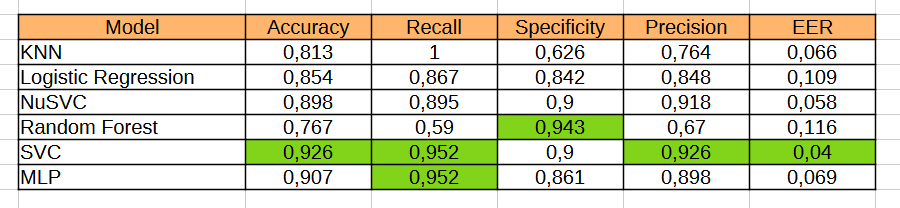
\includegraphics[width=0.8\textwidth]{Images/Results/Verification_single/ft/VB_FA_LIT.png}
    \label{tab:VB_FA_LIT_ft}
\end{table}

The Table \ref{tab:VB_FA_LIT_ft} illustrates that the best-performing animation, in terms of accuracy, is VB\_FA\_SMA, achieving an accuracy of 92.6\% with the SVC classifier and an EER of 4\%.

\begin{table}[ht]
    \centering
    \caption{Verification results using the Full Train (FT) configuration and VB\_FA\_BIG animation.}
    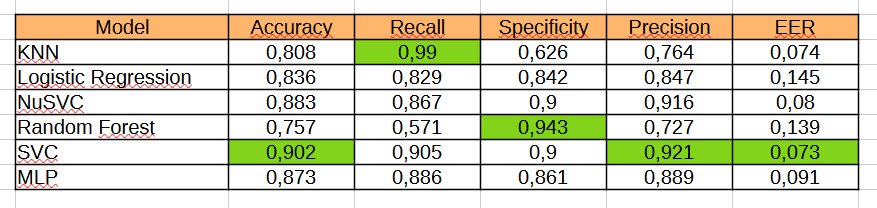
\includegraphics[width=0.8\textwidth]{Images/Results/Verification_single/ft/VB_FA_BIG.png}
    \label{tab:VB_FA_BIG_ft}
\end{table}

The next best-performing animation is VB\_FA\_BIG. 
As illustrated in Table \ref{tab:VB_FA_BIG_ft}, it attains an accuracy of 90.2\% with the SVC classifier and an EER of 7.3\%. 
Results for the remaining animations are provided in Appendix \ref{subsec:vs_ft}

\begin{figure}[ht]
    \centering
    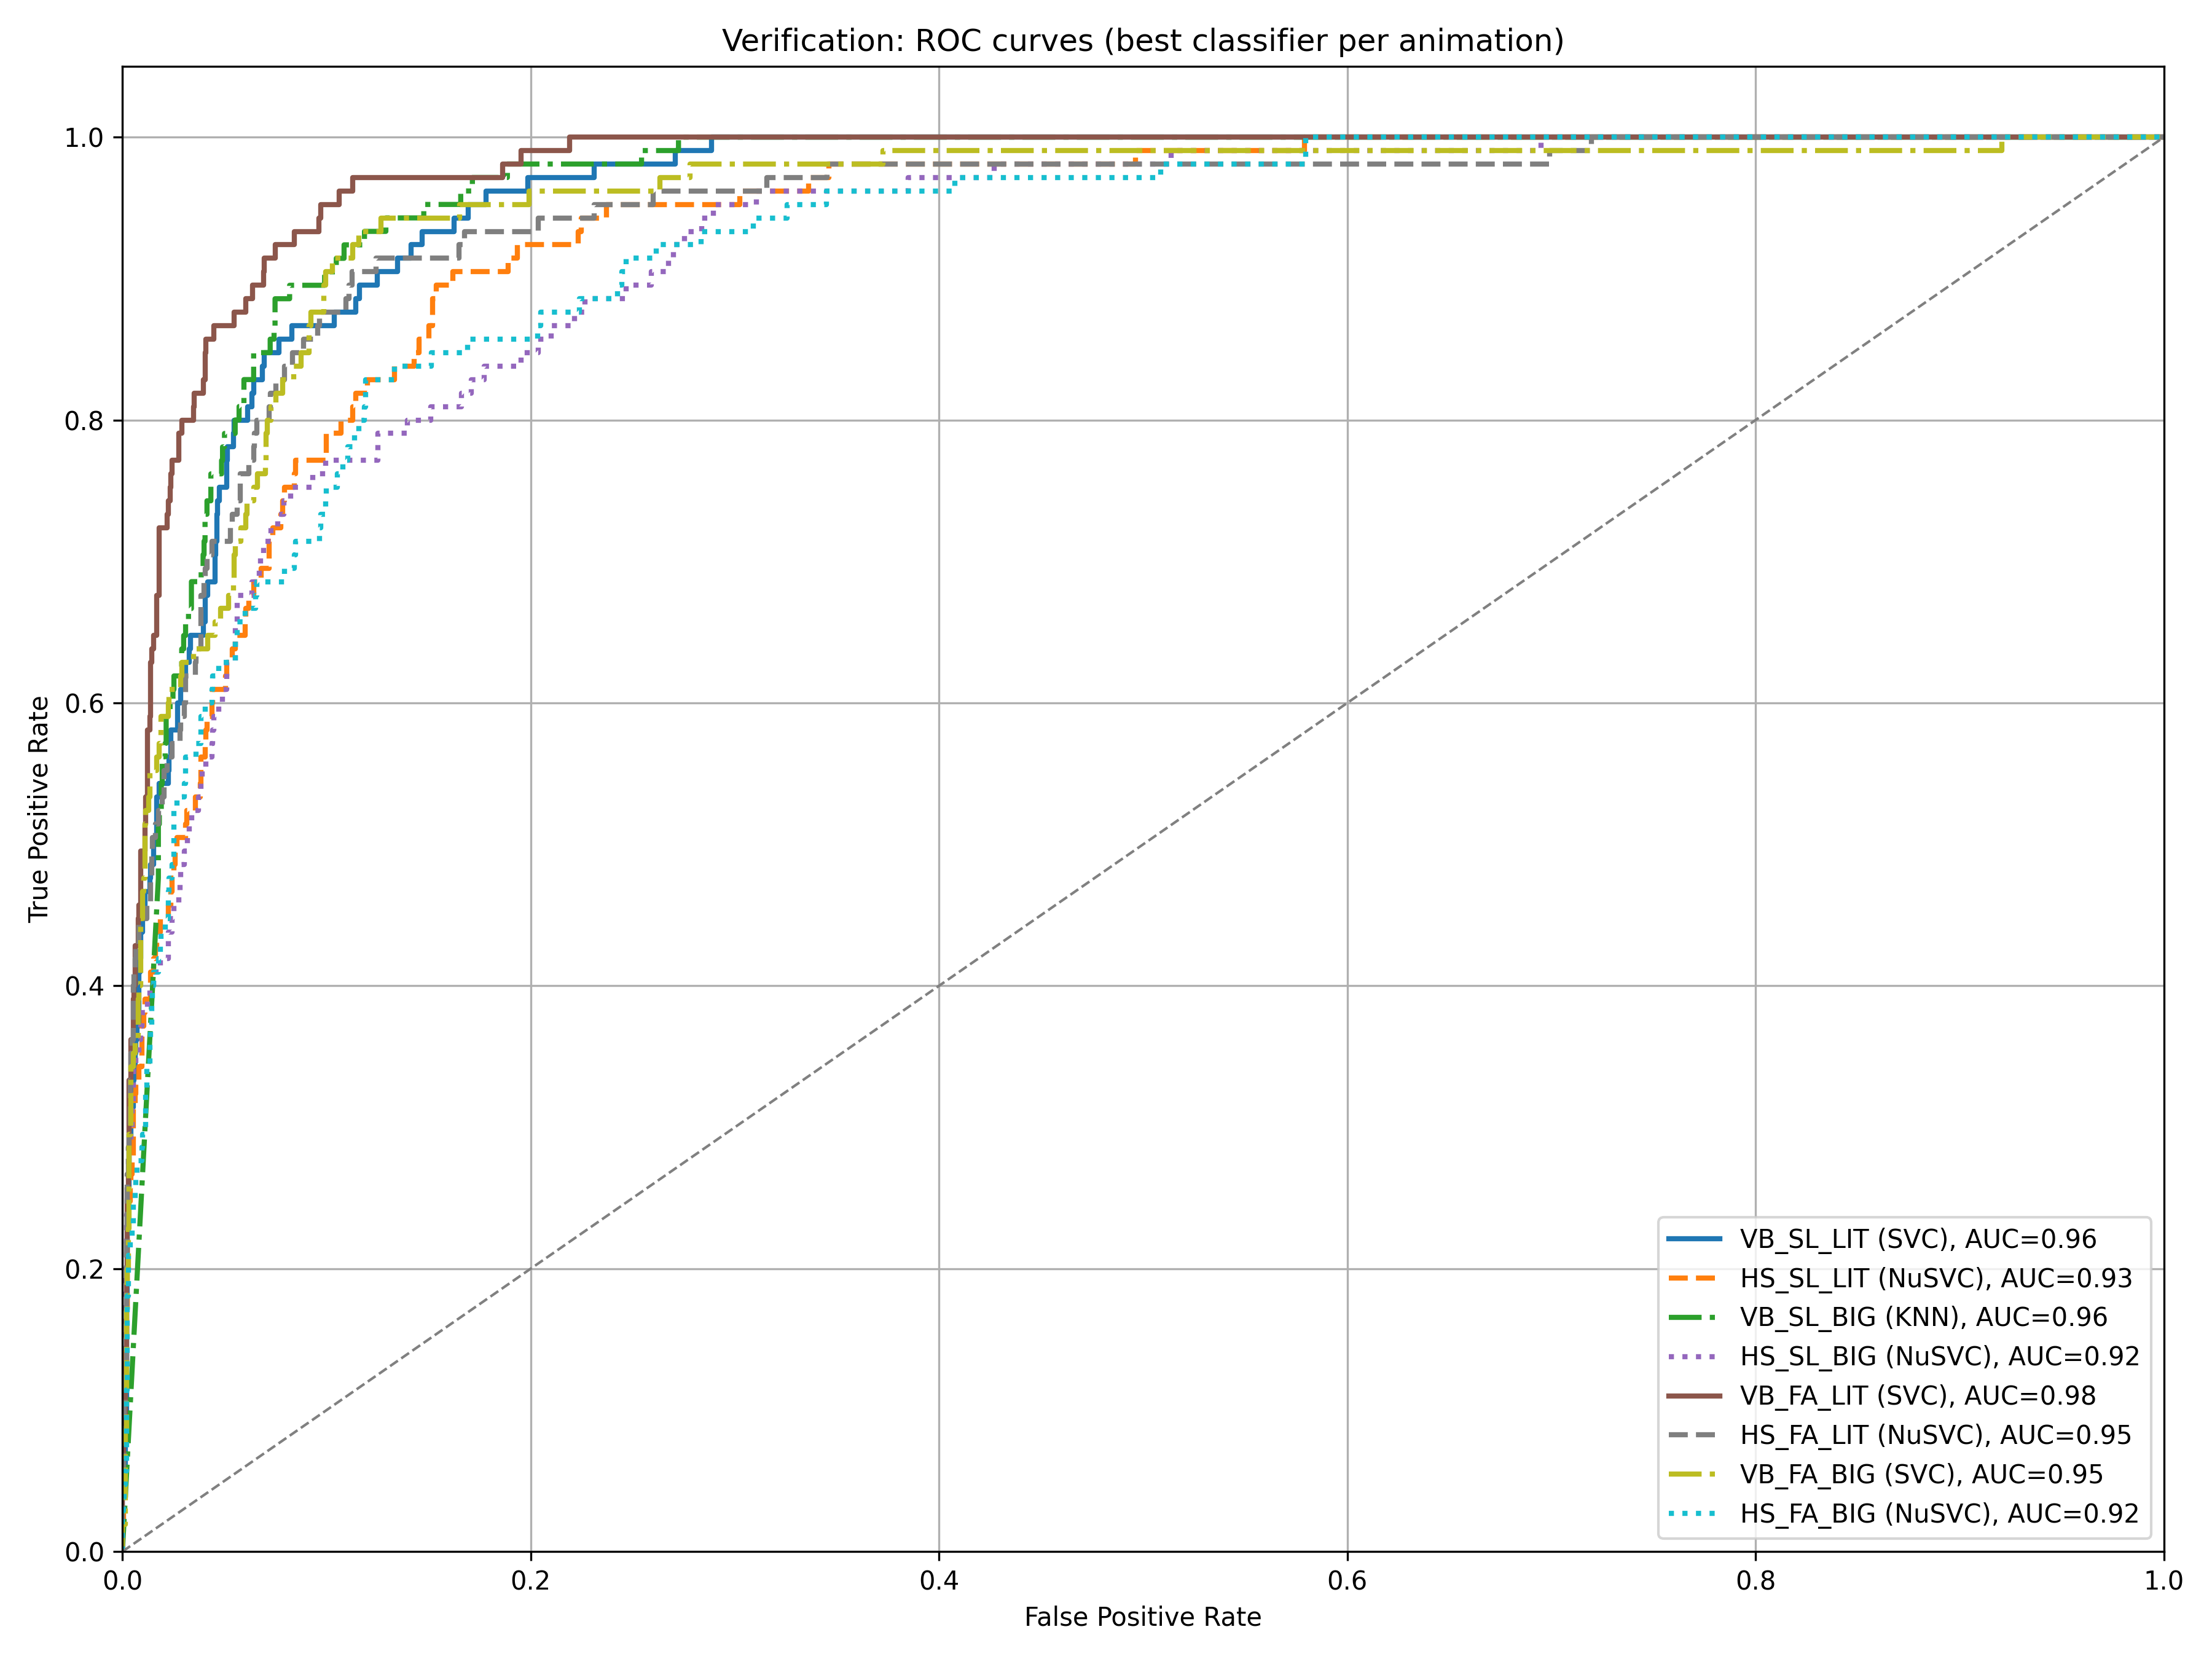
\includegraphics[width = 0.6
    \textwidth]{Images/Results/Verification_single/ft/best_animation_roc_curves_ft.png}
    \caption{ROC curves.}
    \label{fig:roc_ft}
\end{figure}

The figure \ref{fig:roc_ft} shows the ROC curves for each animation, generated using the classifier that achieved the lowest Equal Error Rate. 
The legend for each curve also includes the corresponding Area Under the Curve (AUC) value, serving as an additional measure of performance.

To conclude this section, we present a comparison between the results obtained here and those discussed in Section \ref{subsec:vs_st}. 
Considering all animations, the current analysis outperforms the previous one in six out of eight cases. 
Nevertheless, the overall results are quite close, with differences of less than ten percentage points.

When comparing the best-performing animations from each analysis, the VB\_FA\_SMA animation in this study achieves higher accuracy than the VB\_FA\_BIG animation from the previous analysis. 
Specifically, the Support Vector Classifier (SVC) yields an accuracy of 92.6\%, compared to 92.2\% obtained with the Random Forest classifier. 
However, the EER increases slightly in this analysis—from 3.6\% in the previous section to 4\%.

Therefore, the choice between the two approaches depends on whether higher accuracy or greater security is prioritized for the intended implementation. 
It is also important to note that the present analysis requires data collection over three different sessions, covering eight animations of 15 seconds each, whereas the previous analysis used only a single animation for model training.
\FloatBarrier

\subsection{Verification single animation with intruders - Full Train(FT)}
\label{subsec:intruders}

Following the completion of the closed-set verification analysis for the single animation and Full Train (FT) configuration, we next conduct the open-set analysis. 
The purpose of this evaluation is to assess the system’s performance when confronted with test data originating from users who were not part of the training process. 
Essentially, this scenario represents an unauthorized individual attempting to gain access to a system without having a registered identity.

Similar to the earlier experiments, all classifiers are trained using the optimal hyperparameters determined during the identification stage. 
The dataset is restricted to the top k selected features to minimize computational demands. 
In this configuration, the set of 35 participants is split into 24 enrolled users, representing authorized members, and 11 impostors, comprising roughly one-third of the sample. 
This partition is established using a fixed random seed to guarantee reproducibility of results across multiple runs.

For each of the 24 enrolled users, a separate model is trained using the user’s genuine samples for every animation, drawn from the first two recording sessions (S1 and S2).
The train set is then completed with the same length of feature vectors that come from other users, registered in the system, S1 and S2 data.
Then we repeat this process for 20 different seeds, we train all these model and we take the best based on their training accuracy score.

Next, we use the same random seeds to generate twenty different test sets. 
Each test set is created by taking the third session (S3) data of the genuine user for a single animation and adding the Session 3 data randomly sampled from the 11 intruders.
The best-performing model is then evaluated on all twenty test sets. 
Finally, we compute the average performance per seed for each user model. 
Then, we calculate the overall average across all users to determine the general performance of the system.

\begin{table}[ht]
    \centering
    \caption{Verification results with intruders using the Full Train (FT) configuration and VB\_FA\_SMA animation.}
    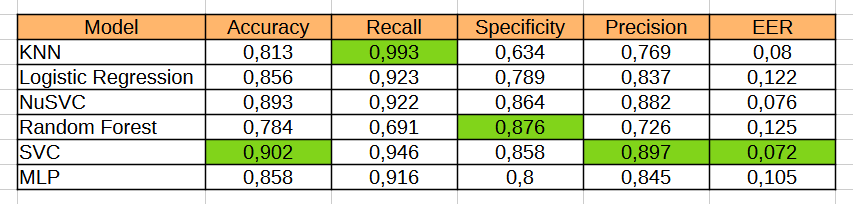
\includegraphics[width=0.8\textwidth]{Images/Results/Verification_single_intruders/ft/VB_FA_LIT.png}
    \label{tab:VB_FA_LIT_fti}
\end{table}

The Table \ref{tab:VB_FA_LIT_fti} shows that the VB\_FA\_SMA animation yields the highest accuracy among all tested cases, reaching 90.2\% when using the SVC classifier. 
The corresponding EER for this configuration is 7.2\%.

\begin{table}[ht]
    \centering
    \caption{Verification results with intruders using the Full Train (FT) configuration and VB\_FA\_BIG animation.}
    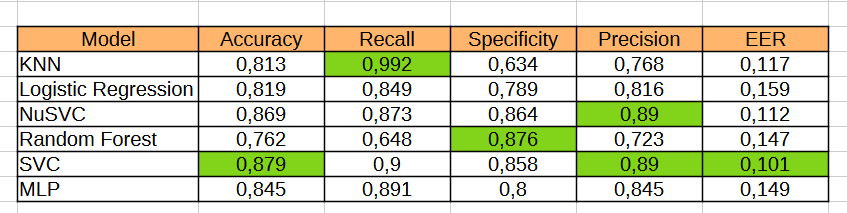
\includegraphics[width=0.8\textwidth]{Images/Results/Verification_single_intruders/ft/VB_FA_BIG.png}
    \label{tab:VB_FA_BIG_fti}
\end{table}

The second-best performance is obtained with the VB\_FA\_BIG animation. 
As shown in Table \ref{tab:VB_FA_BIG_fti}, this configuration achieves an accuracy of 87.9\% when using the SVC classifier, along with an EER of 10.1\%. 
The results for the other animations are reported in Appendix \ref{subsec:vsi_ft}.


\begin{figure}[ht]
    \centering
    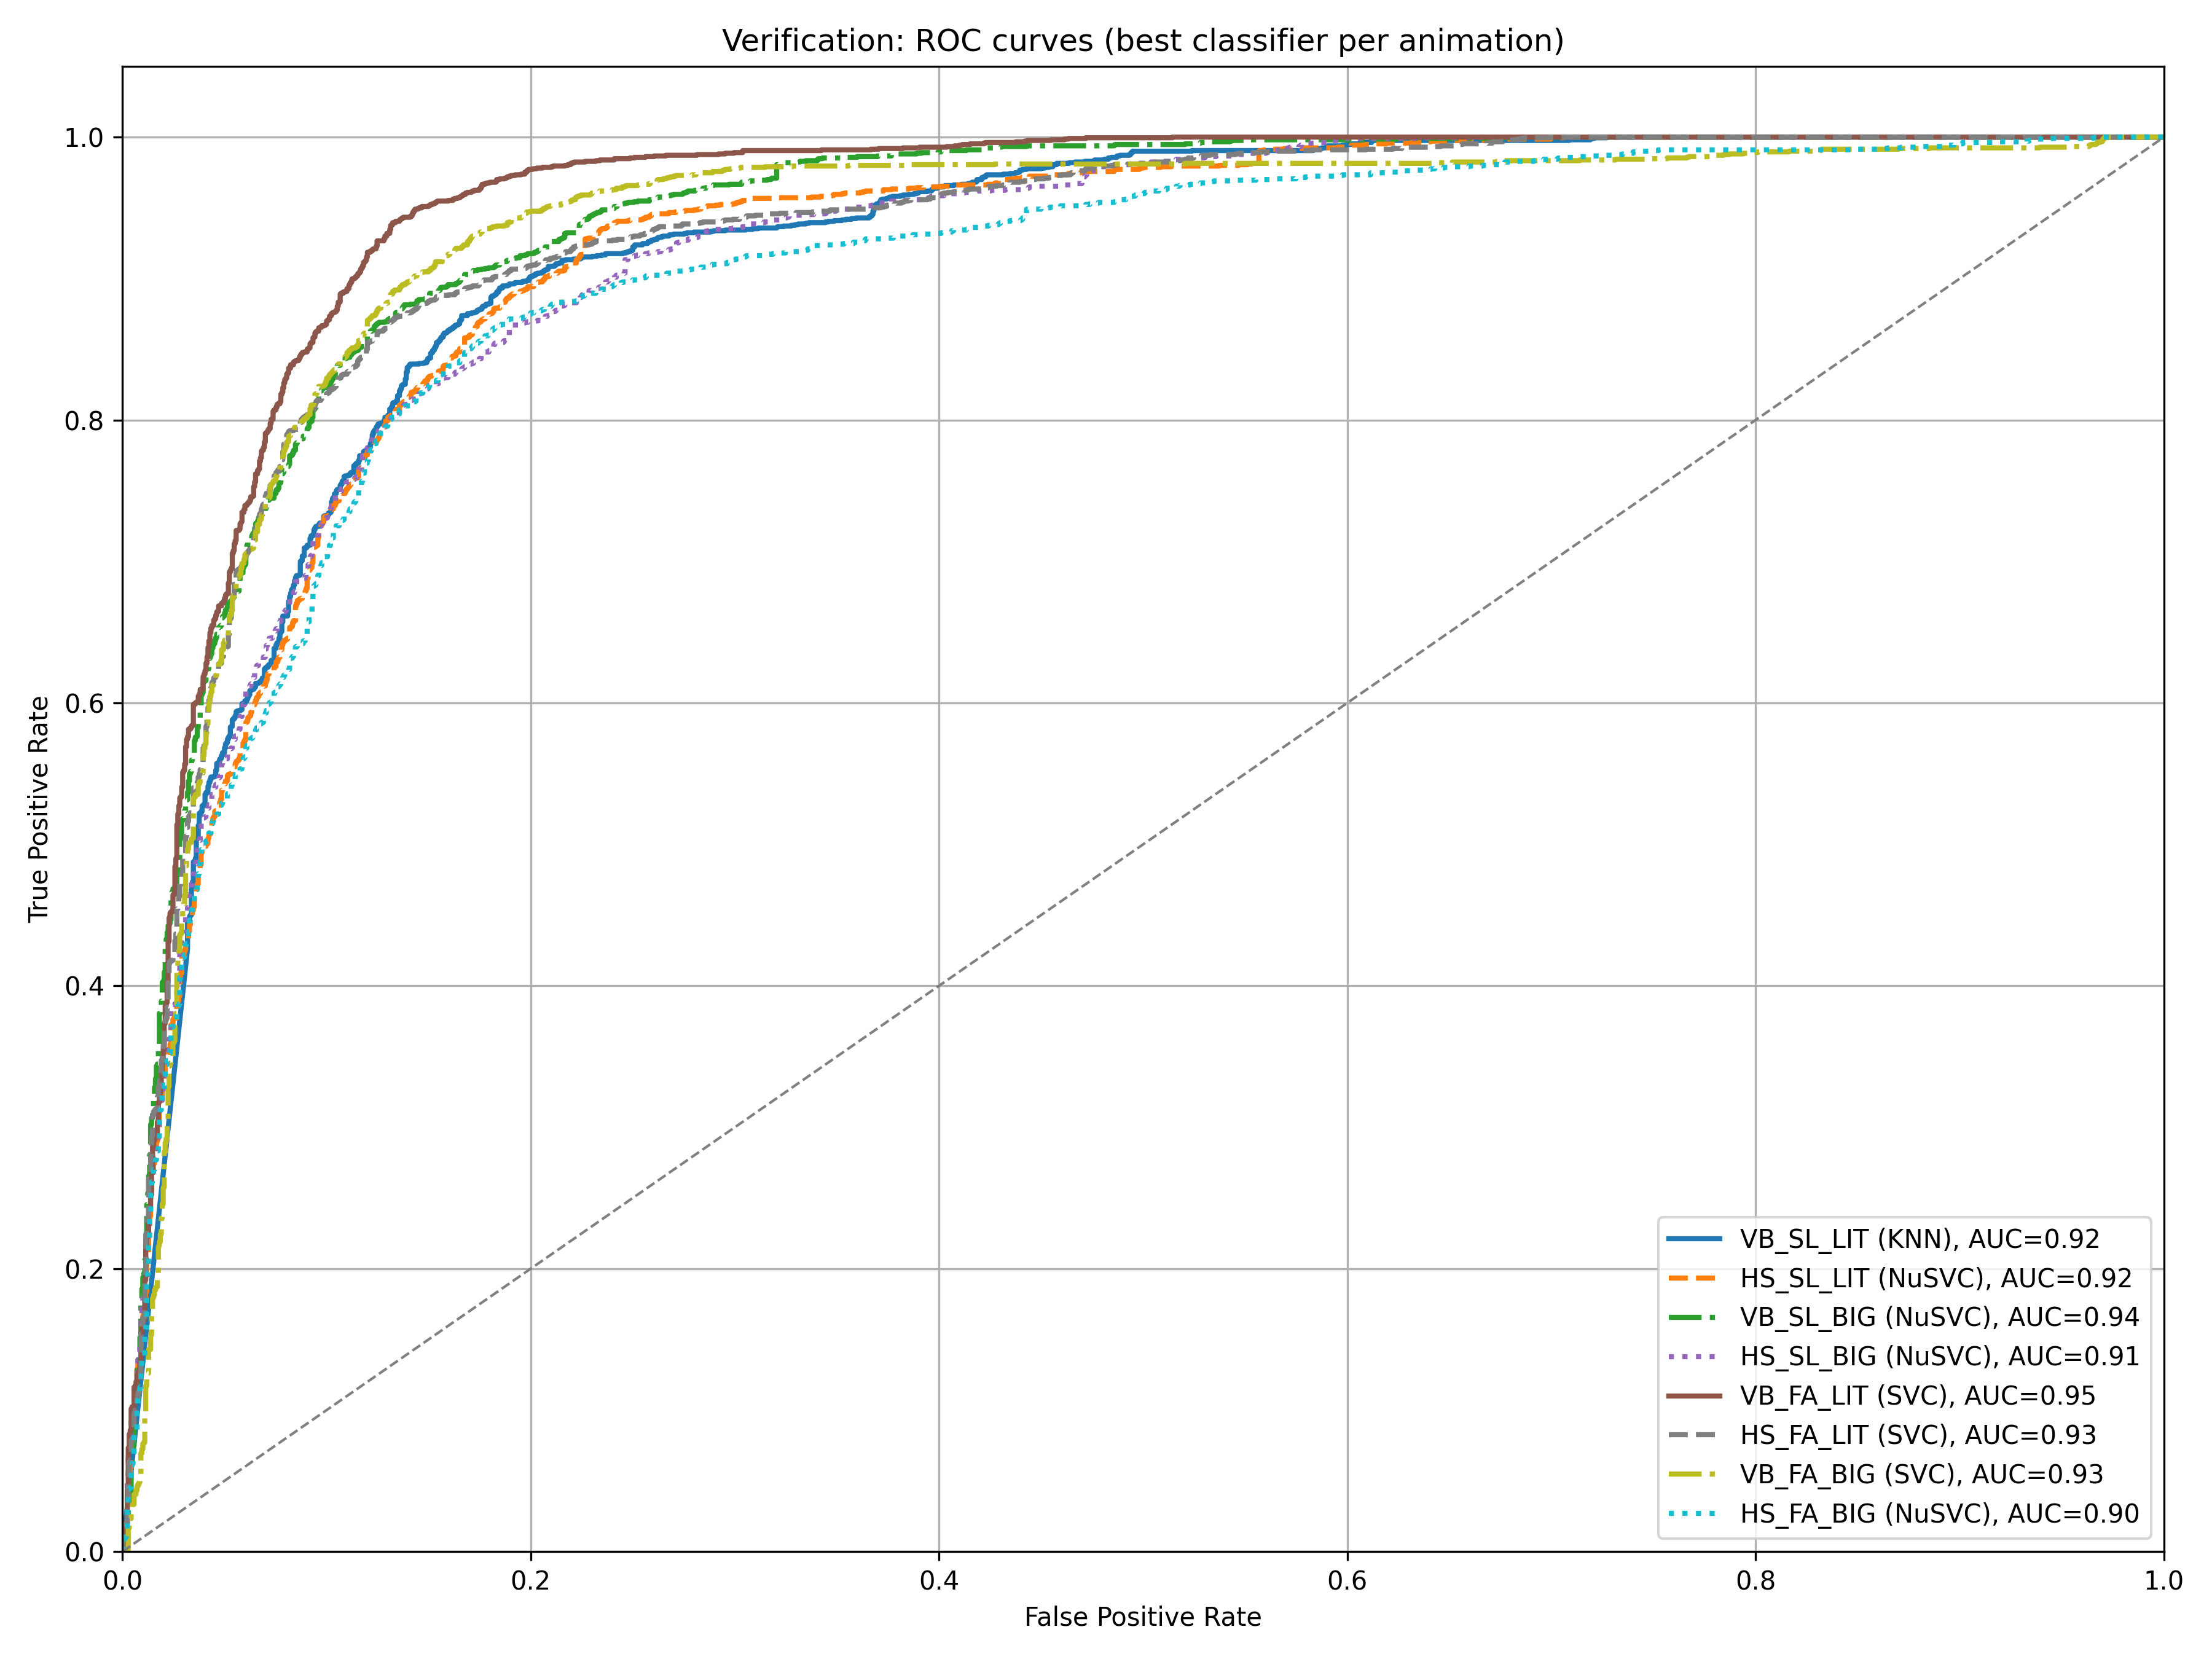
\includegraphics[width = 0.6
    \textwidth]{Images/Results/Verification_single_intruders/ft/best_animation_roc_curves_ft.png}
    \caption{ROC curves.}
    \label{fig:roc_fti}
\end{figure}

The figure \ref{fig:roc_fti} displays the ROC curves obtained from the analysis.

When comparing these results with those obtained in the corresponding analysis including intruders, the best-performing animation remains VB\_FA\_SMA. 
In the open-set configuration, its accuracy decreases from 92.6\% to 90.2\% using the SVC classifier, while the EER rises from 4\% to 7.2\%. 
This performance drop is expected due to the introduction of previously unseen users. 
Nonetheless, the model continues to demonstrate strong performance, maintaining an accuracy above 90\%.

When comparing this analysis with its counterpart presented in Section \ref{subsec:vsi}, it is observed that no single modality consistently achieves the best performance across all animations. 
However, considering the top-performing animations, the single-train (ST) configuration slightly outperforms the full-train (FT) one. 
Specifically, the ST setup attains an accuracy of 91.2\% compared to 90.2\% using the SVC classifier, and also exhibits a lower EER of 6.1\% versus 7.2\% in the current analysis.
\FloatBarrier

\subsection{Verification Single Animation with Reduced Session Duration - Full Train (FT)}

The purpose of the following section is to extend the single-animation verification using the full-train (FT) configuration, with the aim of assessing how the system’s performance varies when the recording duration is shortened. 
Specifically, the same procedure described in Section \ref{subsec:vft} is applied, with the only change being the composition of the dataset.

In this experiment, the datasets include recordings corresponding to the first ten seconds and the first five seconds of each animation. 
Since the GP3\_HD eye tracker samples at 150 Hz, it captures 150 data points per second, each stored as a separate row in the resulting CSV file. 
Consequently, the dataset for the 10-second condition contains the initial 1,500 samples (150 × 10) of each recording, while the 5-second condition includes the first 750 samples (150 × 5).

This analysis is particularly significant because it investigates how reducing the recording duration impacts the performance of the best-performing animation. 
The objective is to determine an effective balance between accuracy and acquisition time, a critical consideration for practical implementations. 
In real-world scenarios, excessively long animations may lead to a loss of user attention or disengagement, ultimately degrading both data quality and system usability.

\begin{table}[ht]
    \centering
    \caption{Verification results with 10-second recordings using the FT configuration and VB\_FA\_SMA animation.}
    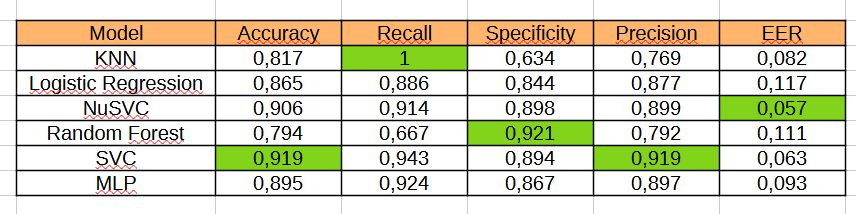
\includegraphics[width=0.8\textwidth]{Images/Results/Verification_single_five_ten/ft/ten/VB_FA_LIT.png}
    \label{tab:VB_FA_LIT_10_ft}
\end{table}

\begin{table}[ht]
    \centering
    \caption{Verification results with 5-second recordings using the FT configuration and VB\_FA\_SMA animation.}
    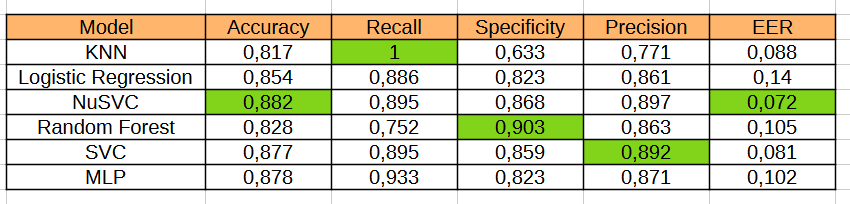
\includegraphics[width=0.8\textwidth]{Images/Results/Verification_single_five_ten/ft/five/VB_FA_LIT.png}
    \label{tab:VB_FA_LIT_5_ft}
\end{table}


In this section, the focus is on evaluating how the performance of the best-performing animation changes as the recording duration is progressively reduced. 
As anticipated, VB\_FA\_SMA continues to be the top-performing animation, confirming the findings from the 15-second analysis.

When the recording time is limited to the first 10 seconds, accuracy shows a slight decrease from 92.6\% to 91.9\% with the SVC classifier, while the EER increases from 4\% to 6.3\%. 
Further shortening the duration to 5 seconds results in an accuracy of 88.2\% using the nuSVC classifier and an EER of 7.2\%.

These outcomes are highly promising, as they indicate that the model preserves robust performance even under substantially shorter acquisition times. 
With a 10-second interval, accuracy remains above 90\%, showing only minor degradation, and the 5-second configuration still achieves a commendable accuracy of 88.2\%.
Depending on the target application and practical limitations, any of these setups may be chosen to achieve an appropriate balance between efficiency and reliability.

The remaining results for the other animations are presented in Appendix \ref{subsec:vs_st_ft_rt}, due to space constraints.

\begin{figure}[ht]
    \centering
    \includegraphics[width = 0.6
    \textwidth]{Images/Results/Verification_single_five_ten/ft/ten/best_animation_roc_curves_ten_ft.png}
    \caption{ROC curves 10 seconds.}
    \label{fig:roc_t_ft}
\end{figure}

\begin{figure}[ht]
    \centering
    \includegraphics[width = 0.6
    \textwidth]{Images/Results/Verification_single_five_ten/ft/five/best_animation_roc_curves_five_ft.png}
    \caption{ROC curvas 5 seconds.}
    \label{fig:roc_f_ft}
\end{figure}

To continue this section, we present the ROC curves derived from the EER values of both analyses. 
Specifically, Figures \ref{fig:roc_t_ft} and \ref{fig:roc_f_ft} correspond to the 10-second and 5-second experiments, respectively.

To assess which configuration provides the best results for the top-performing animation in both the single-train (ST) and full-train (FT) cases, a direct comparison is conducted.
For the 10-second recordings, the FT configuration outperforms the ST one in terms of accuracy, achieving 91.9\% with the SVC classifier and the VB\_FA\_SMA animation, compared to 90.2\% obtained with the Random Forest classifier and the VB\_FA\_BIG animation.
However, the ST configuration maintains a lower EER of 4.5\%, compared to 6.3\% for the FT setup.

When examining the 5-second recordings, both configurations show very similar accuracy results. 
The ST approach reaches 88.8\% using the Random Forest classifier with the VB\_FA\_BIG animation, while the FT setup achieves 88.2\% using the nuSVC classifier with VB\_FA\_SMA.
Again, the ST configuration provides a lower EER, with 6.8\% compared to 7.2\% for the FT case.

When selecting the optimal configuration for the 10-second recordings, the choice depends on whether accuracy or security is prioritized. 
If a lower EER is preferred, the ST configuration is more suitable.
If higher accuracy is the main objective, the FT configuration should be chosen.
Overall, for the 5-second recordings, the ST configuration consistently outperforms the FT one across all scenarios.
\FloatBarrier

\section{Verification ’classic’ single animation - FT type}

The following section presents an analysis analogous to that described in Section \ref{subsec:terza_ver}, with a slight modification to the evaluation procedure.

In this case, the evaluation does not rely on a single optimal model selected from multiple training runs.
Instead, for each individual user, twenty separate models are trained and evaluated independently, each corresponding to a different random seed.
Both the training and testing datasets are generated according to the same seed, ensuring consistency between data partitions.

The motivation behind the previous approach, evaluating all configurations using the globally best model, was to investigate whether this strategy could lead to improved overall performance.
To enable a fair and consistent comparison, the results of this more traditional verification procedure are also reported here.
Finally, it is important to note that this section concludes the verification analysis presented in this work.

\subsection{Verification single animation classic without intruders - Full Train (FT)}

This section, along with the next, presents the 'classic' verification analysis conducted on single animations.
The term classic refers to the fact that this analysis differs from the previous approach, where the evaluation was performed using a single best-performing model.
In this case, each model is trained and tested independently for every random seed.
As in the previous analyses, two levels of averaging are applied. 
The first level of averaging is carried out across all repetitions generated by the different random seeds for each subject-specific model, providing a stable estimate of individual performance. 
The second level aggregates the outcomes of all subject models to assess the overall performance of the system.

This analysis thus serves as a direct counterpart to the one discussed previously in Section \ref{subsec:vft}, maintaining the same Full Train (FT) configuration. 
Consequently, the methodological details remain unchanged and will not be restated. 
The focus instead is on examining the obtained results and comparing them with those from the previous setup to determine which approach yields more stable and effective performance.

As in the preceding analysis, the best-performing animation continues to be VB\_FA\_SMA, attaining an accuracy of 92.4\% with the NuSVC classifier and an EER of 5\%.

\begin{table}[ht]
    \centering
    \caption{Classic verification results using the FT configuration and VB\_FA\_SMA animation.}
    \includegraphics[width=0.8\textwidth]{Images/Results/Classic_procedure/Verification_single/ft/VB_FA_LIT.png}
    \label{tab:VB_FA_LIT_cft}
\end{table}

The Table \ref{tab:VB_FA_LIT_cft} presents the best-performing animation, while the additional results for the remaining animations are provided in Appendix \ref{subsec:vsc_ft}.
The current analysis also includes the ROC curves of the best-performing animations, selected according to their Equal Error Rate, as shown in Table \ref{tab:roc_cft}.

\begin{table}[ht]
    \centering
    \caption{ROC curves.}
    \includegraphics[width=0.6\textwidth]{Images/Results/Classic_procedure/Verification_single/ft/Verification_single_roc_classic_ft.png}
    \label{tab:roc_cft}
\end{table}

When compared to the previous approach (Section \ref{subsec:vft}), which achieved an accuracy of 92.6\% with the SVC classifier and an EER of 4\% on the same animation, the current method shows slightly lower performance in both accuracy and EER.
\FloatBarrier

\subsection{Verification 'classic' single animation with intruders - Full Train (FT)}

To proceed, we conducted the analysis using unseen users in the test set, referred to as intruders. 
This evaluation follows the closed-set analysis and was performed in the same manner as described in the previous section, with only minor adjustments to the evaluation procedure.

The first notable observation is that the best-performing animation remains the same as in the closed-set analysis, but with a slight decrease in performance due to the presence of the intruders.

\begin{table}[ht]
    \centering
    \caption{‘Classic’ verification with intruders using the FT configuration and VB\_FA\_SMA animation.}
    \includegraphics[width=0.8\textwidth]{Images/Results/Classic_procedure/Verification_intruders/ft/VB_FA_LIT.png}
    \label{tab:VB_FA_LIT_cift}
\end{table}

As shown in Table \ref{tab:VB_FA_LIT_cift}, the accuracy decreases from 92.4\% using nuSVC to 89.2\% when using the SVC classifier.
While the EER increases from 5\% to 8.2\%. 
This reduction in performance is expected due to the introduction of unseen users in the test set. 
Nevertheless, the drop remains relatively modest, indicating that the system continues to operate effectively under this more challenging evaluation scenario.

When comparing these results with the evaluation using the best model (Section \ref{subsec:intruders}), performance remains comparable: 89.2\% versus 90.2\% using SVC. 
In parallel, the EER increases from 7.2\% in the previous analysis to 8.2\% in this one.
In conclusion, the analysis that evaluate only on the 'best model' achieves better performance.

\begin{figure}[ht]
\centering
\includegraphics[width=0.6\textwidth]{Images/Results/Classic_procedure/Verification_intruders/ft/Verification_single_intruders_roc_two_ft.png}
\caption{ROC curves.}
\label{fig:roc_cift}
\end{figure}

For consistency with previous analyses, the ROC curves based on the Equal Error Rate are presented in Figure \ref{fig:roc_cift}. 
Additional results for this evaluation can be found in the corresponding appendix (Appendix \ref{subsec:vsci_ft}).
\FloatBarrier

\subsection{Verification 'classic' Single Animation with Reduced Session Duration - Full Train (FT)}

We conclude this analysis by performing a reduced-duration evaluation, following the approach used in the previous subsection. 
Specifically, we assess how performance changes when the total animation length is shortened from 15 seconds to 10 seconds, and subsequently to 5 seconds.

The results align with our expectations, with VB\_FA\_SMA remaining the best-performing animation in terms of accuracy. 
Interestingly, its accuracy slightly increases from 92.4\% with nuSVC to 92.7\% with SVC when the recording duration is reduced to 10 seconds. 
Conversely, its EER rises modestly from 5\% to 5.4\%. 
This suggests that the additional seconds in the longer recording may introduce some noise, slightly affecting the EER, while the accuracy benefits from the initial portion of the animation. 
It is likely that after the first ten seconds, the animation scrolls too quickly for the user to follow effectively, providing limited useful information. 
In contrast, for 15-second recordings, the EER decreases due to the availability of more data, which improves the system’s discriminative power.

When recordings are limited to the first 5 seconds, performance decreases to 90.6\%, and the EER rises to 6.4\%. 
These results highlight a trade-off between recording duration and system performance, with only a modest degradation observed for shorter recordings.

The best-performing animations for the 10- and 5-second conditions are illustrated in Tables \ref{tab:VB_FA_LIT_cft_10} and \ref{tab:VB_FA_LIT_cft_5}, respectively. 
The corresponding ROC curves for these conditions are presented in Figures \ref{fig:roc_cft_10} and \ref{fig:roc_cft_5}.
Additional results and supporting material for this analysis are provided in Appendix \ref{subsec:vsc_ftr}.

\begin{table}[ht]
    \centering
    \caption{Verification ’classic’ results with 10-second recordings using the FT configuration and VB\_FA\_SMA animation.}
    \includegraphics[width=0.8\textwidth]{Images/Results/Classic_procedure/five_ten/ft/ten/VB_FA_LIT.png}
    \label{tab:VB_FA_LIT_cft_10}
\end{table}

\begin{table}[ht]
    \centering
    \caption{Verification ’classic’ results with 5-second recordings using the FT configuration and VB\_FA\_SMA animation.}
    \includegraphics[width=0.8\textwidth]{Images/Results/Classic_procedure/five_ten/ft/five/VB_FA_LIT.png}
    \label{tab:VB_FA_LIT_cft_5}
\end{table}


\begin{figure}[ht]
    \centering
    \includegraphics[width = 0.6
    \textwidth]{Images/Results/Classic_procedure/five_ten/ft/ten/Verification_single_roc_ten_classic_ft.png}
    \caption{ROC curves - 10 seconds.}
    \label{fig:roc_cft_10}
\end{figure}

\begin{figure}[ht]
    \centering
    \includegraphics[width = 0.6
    \textwidth]{Images/Results/Classic_procedure/five_ten/ft/five/Verification_single_roc_five_classic_ft.png}
    \caption{ROC curves - 5 seconds.}
    \label{fig:roc_cft_5}
\end{figure}

To conclude this section, we compare the results of the current analysis with those from the previous section, performed under the same reduced time conditions.
For the ten-second recordings, the current procedure slightly outperforms the previous one, achieving an accuracy of 92.7\% compared to 91.9\% obtained using SVC. 
The EER also improves, decreasing from 6.3\% to 5.4\%.

For the five-second recordings, a similar trend is observed. 
The current analysis reaches a higher accuracy of 90.6\%, compared to 88.2\% in the previous evaluation, while the EER decreases from 7.2\% to 6.4\%.
In summary, this evaluation generally surpasses the previous approach in all aspects, demonstrating better performance across both accuracy and EER.

\FloatBarrier

\section{Static vs Dynamic text}
\label{subsec:s_vs_d}

The final part of the machine learning analysis presents a direct comparison between static and dynamic text under comparable experimental conditions.
Data collection was conducted with eight participants, comprising seven males and one female, the majority of whom were laboratory staff.
Among the participants, three were aged between 20 and 30 years, one between 31 and 40 years, one between 41 and 50 years, two between 51 and 60 years, and one participant was over 60 years old.
Additionally, five participants wore eyeglasses, while none used contact lenses.

\begin{table}[ht]
    \centering
    \caption{Data from Participants Involved in the Experiment.}
    \includegraphics[width=0.7\textwidth]{Images/Experiment/static_vs_dynamic.png}
    \label{tab:tester_8}
\end{table}

A detailed overview is presented in Table \ref{tab:tester_8}.

The presented stimuli differ in order to represent the characteristics of the two text modalities: static and dynamic.
The dynamic text consists of two types of animations, Vertical Block and Horizontal Scroll, each combined with two display speeds and two character sizes, resulting in a total of eight animations. 
These are the same stimuli described in Section \ref{subsec:stimuli}.

In contrast, the static text includes only two animations, both derived from the Vertical Block configuration.
The Horizontal Scroll format was excluded, as displaying a static line of text without movement would eliminate the purpose and meaning of the scrolling mechanism.

The animations used for the static text are:
\begin{itemize}
\item Vertical Block – Big: This animation displays text occupying two-thirds of the screen width, with a font size of 60 pixels. 
It mirrors the dynamic version of the same animation.
However, instead of vertically scrolling text, the full content is visible from the start.
\item Vertical Block – Small: This animation is a smaller variant of the Vertical Block used in the dynamic condition. 
It also occupies two-thirds of the screen width, featuring a static text block with a font size of 30 pixels.
\end{itemize}

\begin{figure}[htbp]
    \centering
    \begin{subfigure}[t]{0.45\textwidth}
        \centering
        \includegraphics[width=\linewidth]{Images/Experiment/BIG_static.png}
        \caption{Vertical Block – Big.}
        \label{fig:static_big}
    \end{subfigure}
    \hfill
    \begin{subfigure}[t]{0.45\textwidth}
        \centering
        \includegraphics[width=\linewidth]{Images/Experiment/LIT_static.png}
        \caption{Vertical Block – Small.}
        \label{fig:static_small}
    \end{subfigure}
    \caption{Different types of static animations.}
    \label{fig:statics}
\end{figure}

Prior to the presentation of each animation within a trial, a fixation stimulus consisting of a white cross displayed at the center of a black screen was shown. 
This visual marker served as an anchor point, ensuring that participants’ gaze was directed toward a consistent location before the onset of each animation.

The inclusion of this fixation phase fulfilled two key purposes. 
First, it standardized the initial gaze position across participants and trials, thereby minimizing variability that could compromise gaze-tracking precision. 
Second, it ensured that participants were visually attentive and prepared for the subsequent stimulus. 
Together, these factors enhanced the reliability of the recorded data by controlling for differences in initial eye position, which is a crucial aspect in gaze-based biometric research where even small deviations can affect performance outcomes.

Each trial consisted of two animations, each lasting 15 seconds. 
Before the onset of every animation, a 2-second fixation cross was displayed, resulting in a total duration of 46 seconds per trial.
Each participant completed three trials in a single session, amounting to 138 seconds, equivalent to approximately 2 minutes and 18 seconds per session.
Across the three sessions conducted on the same day, the total experimental exposure time was 414 seconds, corresponding to approximately 6 minutes and 54 seconds of participation.

After data collection, a machine learning analysis was conducted, focusing on both identification and verification tasks.
The first stage involved performing an identification analysis without distinguishing between individual animations.
Two types of data splits were considered: a random split and a session-based split.

In the random split, the entire dataset was randomly divided into 80\% for training and 20\% for testing.
A stratification procedure was applied based on the participant identifier to ensure a balanced distribution of samples across users, meaning that each participant contributed approximately 80\% of their data to the training set and 20\% to the test set.
This process was repeated ten times to obtain averaged results and reduce the influence of chance variations due to any specific random split.

In contrast, the session split approach used the data from the first two sessions (S1 and S2) for training and the data from the third session (S3) for testing.
This configuration allows for assessing the model’s robustness when applied to data collected at different times.

A GridSearchCV procedure was employed for both datasets to optimize hyperparameters, with the feature selection step omitted for simplicity.
The classifiers and their corresponding parameter grids are presented in Appendix \ref{subsec:param}.

\begin{table}[htbp]
    \centering
    \caption{Identification results}
    \begin{subfigure}[t]{0.49\textwidth}
        \centering
        \includegraphics[width=\linewidth]{Images/Results/Static_Dynamic/id_moving.png}
        \caption{Identification with dynamic text.}
        \label{tab:dyn_id}
    \end{subfigure}
    \hfill
    \begin{subfigure}[t]{0.49\textwidth}
        \centering
        \includegraphics[width=\linewidth]{Images/Results/Static_Dynamic/id_stat.png}
        \caption{Identification with static text.}
        \label{tab:stat_id}
    \end{subfigure}
\end{table}

The Tables \ref{tab:dyn_id} and \ref{tab:stat_id} shows the results obtained during the identification analysis. 
In general, random splits yield higher accuracies compared to the static text stimuli. 
For instance, the best result with this split is achieved using SVC, reaching an accuracy of 93.1\% for the static variation, whereas dynamic text reaches 90.78\% with an MLP classifier.

The interesting property of the dynamic text is the way in which the results scale down with session split. 
Even if static text reaches an accuracy of 85.42\% using MPL we can see that the overall results are generally lower than dynamic text variation. 
As we noticed earlier, in fact dynamic text stimuli mantain a comparable performance between random split and session split. 
This is very important for us because session split will be the mode we will use in real-life application. 
The peak with this split is reached with 86.46\% using nuSVC.

It should also be noted that the relatively high accuracies are partially due to the limited number of testers involved, which simplifies both identification and verification tasks. 
Nevertheless, under similar experimental conditions, dynamic text stimuli demonstrate a promising property.

We now move to the verification analysis to examine whether the properties observed in the identification stage are maintained in this context.
The classifiers and the parameters used for hyperparameter tuning through GridSearchCV are the same as those described in the previous identification process.

In verification, a separate model is trained for each user, and the same two data split strategies are employed, with some adaptations.

For the random split, the training set for each model is composed of 80\% of the genuine user’s data, combined with an equal number of feature vectors randomly sampled from other users. 
The model is then tested on the remaining 20\% of the genuine users data, together with an equal number of impostor samples not used during training.
This process is repeated ten times with different random seeds to reduce randomness, and the final results represent the average performance across all trials.

The session split is executed only once. 
In this case, the training set consists of the data from the first two sessions (S1 and S2) of the genuine user, along with an equal number of samples randomly drawn from other users. 
The test set includes the data of the third session (S3) of the genuine user and an equal amount of S3 data from impostors.
The model is then evaluated on this configuration, and the results provide the average performance under this type of split.

For this analysis, in addition to accuracy, precision, recall, specificity, and Equal Error Rate are also reported to provide a comprehensive evaluation of system performance.

\begin{table}[ht]
    \centering
    \includegraphics[width=0.6\textwidth]{Images/Results/Static_Dynamic/Ver_mov.png}
    \caption{Verification with dynamic text.}
    \label{tab:ver_dyn}
\end{table}

\begin{table}[ht]
    \centering
    \includegraphics[width=0.6\textwidth]{Images/Results/Static_Dynamic/Ver_stat.png}
    \caption{Verification with static text.}
    \label{tab:ver_stat}
\end{table}

The results of the verification analysis for dynamic and static text are presented in Table \ref{tab:ver_dyn} and Table \ref{tab:ver_stat}, respectively.
As shown, under the random split, the static text stimuli achieve slightly better performance, reaching an accuracy of 93.59\% with the Random Forest classifier, compared to 92.5\% for the dynamic text. 
The Equal Error Rate follows the same trend, with the static text achieving 2.81\% versus 6.36\% for the dynamic variation.

When examining the session split, we observe that the same property highlighted earlier still holds.
Namely, the performance difference between random and session splits remains relatively small.
In this case, the dynamic text reaches an accuracy of 92.19\% with the MLP classifier, compared to 87.5\% achieved by the static text using the same model. 
However, the static text maintains a lower EER (4.17\%) compared to 6.77\% for the dynamic text.
Overall, across both configurations, the static text consistently provides lower EER values, indicating a higher degree of reliability in terms of security performance.

In conclusion, when considering the session split, which reflects the conditions of a real-world application, the dynamic text demonstrates higher accuracy, with minimal or negligible degradation compared to the random split.
Conversely, the static text consistently achieves better EER values, making it more suitable for scenarios where security and low error rates are the primary concern.
Therefore, a behavioral biometric system based on dynamic text is more appropriate when accuracy is the key performance indicator, whereas a static text-based approach is preferable in applications that prioritize security and robustness.

\FloatBarrier
\newpage

\chapter{Conclusion}

The present thesis aimed to investigate an unexplored soft biometric stimulus based on dynamic text. 
To achieve this goal, two types of animations were designed: the Vertical Block Scroll (VB) and the Horizontal Scroll (HS), each implemented with two different scrolling speeds and two font sizes.
This combination produced a total of eight distinct stimuli. 
These animations were presented to thirty-five participants, who completed three trials on the same day, repeated across three separate sessions on different days. 
This experimental design enabled the collection of a rich dataset of eye movement features through an eye-tracking device, providing the foundation for an extensive machine learning analysis.

The first part of the study focused on the identification process, with the objective of evaluating the discriminative capability of the proposed stimuli. 
Although soft biometric traits are most commonly applied in verification systems, several works have demonstrated their suitability for identification as well. 
In this initial evaluation, when all animations were analyzed together, the system achieved a maximum accuracy of 67.62\% using an MLP classifier under the session split configuration. 
This result, while moderate, confirmed the potential of the dynamic text-based stimuli as identifiable behavioral patterns.

Following this, the analysis proceeded with the evaluation of each individual animation, tested under two distinct training modalities: Single Train (ST) and Full Train (FT). 
The best performance in this phase was achieved using the ST configuration with the VB\_FA\_BIG animation, reaching an accuracy of 82.86\% with the SVC classifier. 
This finding suggests that such an animation could be effectively employed in identification scenarios where this level of accuracy is sufficient for the intended application.

The core of the thesis centered on the verification analysis, which constituted the most comprehensive and informative part of the research. 
To ensure a thorough understanding of the system behavior, the verification study was divided into four experimental configurations, encompassing both ST and FT modalities, each examined under two evaluation strategies: one based on the best-performing model and the other evaluating all possible model pairs. 
For each of these settings, additional analyses were conducted under closed-set and open-set conditions, as well as with reduced recording durations of ten and five seconds.

It is important to note that the FT configuration, although more computationally demanding, integrates all animations in the training phase, while the ST configuration relies on a single animation. 
Across all analyses, the best closed-set verification performance was obtained using the VB\_FA\_SMA animation under the FT configuration and best-model evaluation procedure, achieving an accuracy of 92.6\% and an EER of 4\%. 
Conversely, the lowest EER was observed during the ST analysis with best-model evaluation, where the VB\_FA\_BIG animation reached an EER of 3.6\% and an accuracy of 92.2\% using the Random Forest classifier.
These results collectively demonstrate the robustness and reliability of the proposed approach. 
The experiments confirm that dynamic text stimuli can achieve both high accuracy and low error rates, making them a promising candidate for behavioral biometric verification systems. 
Depending on the specific application requirements, different configurations may be preferred: the VB\_FA\_SMA animation proves optimal when maximizing overall accuracy is the main objective, while the VB\_FA\_BIG animation is more suitable when minimizing the error rate is of primary concern.

In the open-set verification analysis, the highest accuracy was obtained using the Single Train (ST) configuration with the best-model evaluation strategy. 
Under this setup, the system achieved an accuracy of 91.9\% with the SVC classifier and an EER of 6.1\%. 
The lowest EER within the same analysis was also achieved under identical conditions and using the same animation. 
Specifically, the NuSVC classifier reached an EER of 5.1\%, maintaining a high accuracy of 91.2\%.

When examining the reduced-time analyses, the best result for the 10-second recordings was recorded under the Full Train (FT) configuration with the pairwise evaluation procedure. 
In this case, the VB\_FA\_SMA animation achieved an accuracy of 92.7\% with the SVC classifier and an EER of 5.4\%. 
The minimum EER for this duration was observed under the ST configuration, also with pairwise evaluation, where the VB\_FA\_BIG animation achieved 91.5\% accuracy using NuSVC, with an EER of 4.1\%.

For the 5-second recordings, the best overall performance, both in terms of accuracy and EER, was achieved during the Verification “Classic” Single Animation with Reduced Session Duration - Full Train (FT) analysis. 
In this case, the VB\_FA\_SMA animation reached an accuracy of 90.6\% with the NuSVC classifier and an EER of 6.4\%.

Finally, a comparative analysis was conducted between dynamic and static text stimuli under similar experimental conditions.
From this evaluation, two key observations emerged.
First, the performance drop between the random split and session split was found to be minimal, and in some cases even negligible, when using dynamic text stimuli.
This indicates that dynamic text maintains a consistent level of performance even when evaluated across different sessions, a valuable property for real-world biometric applications.
Second, the Equal Error Rate consistently remained lower for static text stimuli compared to their dynamic counterparts, suggesting that static text provides a slightly stronger level of security and discrimination.

In terms of quantitative results, the best performance for dynamic text in the verification task was obtained using the MLP classifier, achieving an accuracy of 92.19\% with an EER of 6.77\%.
Conversely, the static text stimuli reached an accuracy of 87.5\%, also using MLP, but with a lower EER of 4.17\%.
These findings highlight a trade-off between robustness and precision, where dynamic text offers greater consistency across sessions, while static text provides enhanced reliability in terms of error rate.

Another important aspect to highlight is that the vertical block–based animations consistently achieved better results than the horizontal scroll–based ones across nearly all experimental conditions.

In conclusion, the findings of this work demonstrate that dynamic text animations represent a promising and effective stimulus for behavioral biometric applications, offering both reliability and adaptability for real-world user authentication systems.

\newpage

\chapter*{References}
\addcontentsline{toc}{chapter}{References}
\begin{raggedright}

\textit{Note: All web pages and online resources cited above were available and accessible as of October 14, 2025.}

[1] Statista. (2023). Number of smartphone mobile network subscriptions worldwide from 2016 to 2023, with forecasts from 2023 to 2028. \url{https://www.statista.com/statistics/330695/number-of-smartphone-users-worldwide/}

[2] National Institute of Standards and Technology (NIST). (2004). NIST study shows computerized fingerprint matching is highly accurate. \url{https://www.nist.gov/news-events/news/2004/07/nist-study-shows-computerized-fingerprint-matching-highly-accurate}

[3] NEC Corporation. (2021). NIST study shows computerized fingerprint matching is highly accurate. \url{https://www.nec.com/en/press/202109/global_20210922_02.html#:~:text=In%20this%20benchmark%20test%2C%20the,a%20million%20people%20(*2).}

[4] Wang, L., \& Geng, X. (2009). \textit{Behavioral Biometrics for Human Identification: Intelligent Applications.} University of Melbourne, Australia; Southeast University, China. IGI Global.

[5] Al-Zubi, S., Brömme, A., \& Tönnies, K. (2003, September 10–12). Using an active shape structural model for biometric sketch recognition. In \textit{Proceedings of the DAGM Conference} (pp. 187–195). Magdeburg, Germany.

[6] Stolfo, S. J., Hu, C.-W., Li, W.-J., Hershkop, S., Wang, K., \& Nimeskern, O. (2003). Combining behavior models to secure e-mail systems (No. CU Tech. Rep.). Columbia University.

[7] Spafford, E. H., \& Weeber, S. A. (1992, October). Software forensics: Can we track code to its authors? In \textit{Proceedings of the 15th National Computer Security Conference} (pp. 641–650).

[8] Yampolskiy, R. V., \& Govindaraju, V. (2006, April 17–22). Use of behavioral biometrics in intrusion detection and online gaming. In \textit{Biometric Technology for Human Identification III, SPIE Defense and Security Symposium}. Orlando, FL.

[9] Bergadano, F., Gunetti, D., \& Picardi, C. (2002). User authentication through keystroke dynamics. \textit{ACM Transactions on Information and System Security, 5}(4), 367–397. doi:10.1145/581271.581272

[10] Denning, D. E. (1987). An intrusion-detection model. \textit{IEEE Transactions on Software Engineering, 13}(2), 222–232. doi:10.1109/TSE.1987.232894

[11] Garg, A., Rahalkar, R., Upadhyaya, S., \& Kwiat, K. (2006, June 21–23). Profiling users in GUI based systems for masquerade detection. In \textit{Proceedings of the 7th IEEE Information Assurance Workshop (IAWorkshop 2006)}. West Point, NY.

[12] Novikov, D. (2005). Neural networks to intrusion detection. Unpublished MS thesis, Rochester Institute of Technology, Rochester, NY.

[13] Westeyn, T., Pesti, P., Park, K., \& Starner, T. (2005, July). Biometric identification using song-based eye blink patterns. In \textit{Proceedings of the Human Computer Interaction International (HCII)}. Las Vegas, NV.

[14] Westeyn, T., \& Starner, T. (2004). Recognizing song-based blink patterns: Applications for restricted and universal access. In \textit{Proceedings of the Sixth IEEE International Conference on Automatic Face and Gesture Recognition} (p. 717).

[15] BenAbdelkader, C., Cutler, R., \& Davis, L. (2002). Person identification using automatic height and stride estimation. In *Proceedings of the 2002 International Conference on Pattern Recognition* (pp. 377–380, Vol. 4). Quebec City, QC, Canada. doi:10.1109/ICPR.2002.1047474

[16] Kale, A., Sundaresan, A., Rajagopalan, A. N., Cuntoor, N., RoyChowdhury, A., Kruger, V., et al. (2004). Identification of humans using gait. \textit{IEEE Transactions on Image Processing, 13}(9). doi:10.1109/TIP.2004.832865

[17] Erdogan, H., Ercil, A., Ekenel, H., Bilgin, S., Eden, I., \& Kirisci, M. (2005a). Multimodal person recognition for vehicular applications. \textit{Lecture Notes in Computer Science, 3541}, 366–375.

[18] Erdogan, H., Ozyagci, A. N., Eskil, T., Rodoper, M., Ercil, A., \& Abut, H. (2005b, September). Experiments on decision fusion for driver recognition. In \textit{Biennial on DSP for in-vehicle and mobile systems}. Sesimbra, Portugal.

[19] Erzin, E., Yemez, Y., Tekalp, A. M., Erçil, A., Erdogan, H., \& Abut, H. (2006). Multimodal person recognition for human-vehicle interaction. \textit{IEEE MultiMedia, 13}, 18–31. doi:10.1109/MMUL.2006.37

[20] Brause, R., Langsdorf, T., \& Hepp, M. (1999). Neural data mining for credit card fraud detection. In \textit{Proceedings of the 11th IEEE International Conference on Tools with Artificial Intelligence} (pp. 103–106).

[21] Duchowski, A. T. (2017). \textit{Eye Tracking Methodology: Theory and Practice} (3rd ed.). Springer.

[22] Young, L. R., \& Sheena, D. (1975). Survey of eye movement recording methods. \textit{Behavior Research Methods \& Instrumentation, 7}, 397–429. doi:10.3758/BF03201553

[23] Crane, H. D. (1994). The Purkinje image eyetracker, image stabilization, and related forms of stimulus manipulation. In D. H. Kelly (Ed.), \textit{Visual Science and Engineering: Models and Applications} (pp. 13–89). New York: Marcel Dekker.

[24] Crane, H. D., \& Steele, C. M. (1985). Generation-V dual-Purkinje-image eyetracker. \textit{Applied Optics, 24}, 527–537.

[25] Cantoni, V., Nugrahaningsih, N., \& Porta, M., \& Wang, H. (2017). Biometric authentication to access controlled areas through eye tracking. In M. De Marsico, M. Nappi, \& H. Proença (Eds.), *Human Recognition in Unconstrained Environments* (pp. 197–216). Academic Press. doi:10.1016/B978-0-08-100705-1.00009-9

[26] Maeder, A., Fookes, C., \& Sridharan, S. (2004). Gaze-based user authentication for personal computer applications. In \textit{Proceedings of 2004 International Symposium on Intelligent Multimedia, Video and Speech Processing} (pp. 727–730).

[27] Komogortsev, O. V., Karpov, A., \& Price, L. R., Aragon, C. (2012). Biometric authentication via oculomotor plant characteristics. In \textit{2012 5th IAPR International Conference on Biometrics (ICB)} (pp. 413–420).

[28] De Luca, A., Weiss, R., Hußmann, H., \& An, X. (2008). EyePass– eye-stroke authentication for public terminals. In \textit{CHI '08 Extended Abstracts on Human Factors in Computing Systems (CHI EA '08)} (pp. 3003–3008).

[29] Dunphy, P., Fitch, A., \& Olivier, P. (2008). Gaze-contingent passwords at the ATM. In \textit{4th Conference on Communication by Gaze Interaction (COGAIN)} (pp. 59–62).

[30] Weaver, J., Mock, K., \& Hoanca, B. (2011). Gaze-based password authentication through automatic clustering of gaze points. In \textit{2011 IEEE International Conference on Systems, Man, and Cybernetics (SMC)} (pp. 2749–2754).

[31] Cymek, D. H., Venjakob, A. C., Ruff, S., Lutz, O. H.-M., Hofmann, S., \& Roetting, M. (2014). Entering PIN codes by smooth pursuit eye movements. \textit{Journal of Eye Movement Research, 7}(1), Technische Universität Berlin.

[32] Cazzato, D., Evangelista, A., Leo, M., Carcagnì, P., \& Distante, C. (2016). A low-cost and calibration-free gaze estimator for soft biometrics: An explorative study. \textit{Pattern Recognition Letters, 82}, 196–206. doi:10.1016/j.patrec.2015.10.015

[33] Cantoni, V., Galdi, C., Nappi, M., Porta, M., \& Riccio, D. (2015). GANT: Gaze analysis technique for human identification. \textit{Pattern Recognition, 48}(4), 1027–1038. doi:10.1016/j.patcog.2014.02.017

[34] Yin, J., Sun, J., Li, J., \& Liu, K. (2022). An effective gaze-based authentication method with the spatiotemporal feature of eye movement. \textit{Sensors, 22}(8), 3002. doi:10.3390/s22083002

[35] Porta, M., Dondi, P., Zangrandi, N., \& Lombardi, L. (2022). Gaze-Based Biometrics From Free Observation of Moving Elements. \textit{IEEE Transactions on Biometrics, Behavior, and Identity Science, 4}(1), 85–96. doi:10.1109/TBIOM.2021.3130798

[36] Bhatti, O. S., Barz, M., \& Sonntag, D. (2021). EyeLogin - Calibration-free Authentication Method for Public Displays Using Eye Gaze. In \textit{ACM Symposium on Eye Tracking Research and Applications (ETRA '21 Short Papers)}, Article 14, 1–7. doi:10.1145/3448018.3458001

[37] Khamis, M., Trotter, L., Mäkelä, V., von Zezschwitz, E., Le, J., Bulling, A., \& Alt, F. (2018). CueAuth: Comparing Touch, Mid-Air Gestures, and Gaze for Cue-based Authentication on Situated Displays. \textit{Proc. ACM Interact. Mob. Wearable Ubiquitous Technol., 2}(4), Article 174. doi:10.1145/3287052

[38] Malla, A. H. (2018). A Gaze-Based Authentication System: From Authentication to Intrusion Detection. MS Thesis, Texas A\&M University.

[39] Sluganovic, I., Roeschlin, M., Rasmussen, K. B., \& Martinovic, I. (2019). Analysis of Reflexive Eye Movements for Fast Replay-Resistant Biometric Authentication. \textit{ACM Trans. Priv. Secur., 22}(1), Article 4. doi:10.1145/3281745

[40] Fallahi, M., Arias-Cabarcos, P., \& Strufe, T. (2024). Beyond Gaze Points: Augmenting Eye Movement with Brainwave Data for Multimodal User Authentication in Extended Reality. doi:10.48550/arXiv.2404.18694

[41] Alsufyani, N., Ali, A., Hoque, S., \& Deravi, F. (2018). Biometric presentation attack detection using gaze alignment. In \textit{2018 IEEE 4th International Conference on Identity, Security, and Behavior Analysis (ISBA)}, 1–8. doi:10.1109/ISBA.2018.8311472

[42] Lohr, D., Proulx, M. J., Raju, M. H., \& Komogortsev, O. V. (2025). Ocular Authentication: Fusion of Gaze and Periocular Modalities. doi:10.48550/arXiv.2505.17343

[43] D'Amelio, A., Patania, S., Bursic, S., Cuculo, V., \& Boccignone, G. (2023). Using Gaze for Behavioural Biometrics. \textit{Sensors, 23}(3), 1262. doi:10.3390/s23031262

[44] Cantoni, V., Lacovara, T., Porta, M., \& Wang, H. (2018). A Study on Gaze-Controlled PIN Input with Biometric Data Analysis. In \textit{Proceedings of the 19th International Conference on Computer Systems and Technologies (CompSysTech '18)}, 99–103. doi:10.1145/3274005.3274029

[45] Ali, A., Hoque, S., \& Deravi, F. (2021). Directed Gaze Trajectories for Biometric Presentation Attack Detection. \textit{Sensors, 21}(4), 1394. doi:10.3390/s21041394

[46] Ali, A., Hoque, S., \& Deravi, F. (2018). Gaze stability for liveness detection. \textit{Pattern Anal Applic, 21}, 437–449. doi:10.1007/s10044-016-0587-2

[47] Wang, H., \& Cantoni, V. (2018). Gaze-Based Biometrics: Some Case Studies. University of Pavia.

[48] Abdrabou, Y., Shams, A., Mantawy, M. O., Khan, A. A., Khamis, M., Alt, F., \& Abdelrahman, Y. (2021). GazeMeter: Exploring the Usage of Gaze Behaviour to Enhance Password Assessments. In \textit{ACM Symposium on Eye Tracking Research and Applications (ETRA '21 Full Papers)}, Article 9, 1–12. doi:10.1145/3448017.3457384

[49] Harezlak, K., Blasiak, M., \& Kasprowski, P. (2021). Biometric Identification Based on Eye Movement Dynamic Features. \textit{Sensors, 21}(18), 6020. doi:10.3390/s21186020

[50] Wierzbowski, M., Pochwatko, G., Borkiewicz, P., Cnotkowski, D., Pabiś-Orzeszyna, M., \& Kobyliński, P. (2022). Behavioural Biometrics in Virtual Reality: To What Extent Can We Identify a Person Based Solely on How They Watch 360-Degree Videos? In \textit{2022 IEEE International Symposium on Mixed and Augmented Reality Adjunct (ISMAR-Adjunct)}, 417–422. doi:10.1109/ISMAR-Adjunct57072.2022.00090

[51] Casanova, A., Cascone, L., Castiglione, A., Meng, W., \& Pero, C. (2021). User recognition based on periocular biometrics and touch dynamics. \textit{Pattern Recognition Letters, 148}, 114–120. doi:10.1016/j.patrec.2021.05.006

[52] Rubo, M., \& Son, G. (2025). Social gaze fingerprints: identifying social virtual reality users by their eye gaze patterns. \textit{Virtual Reality, 29}, 144. doi:10.1007/s10055-025-01210-4

[53] Silver, D. L., \& Biggs, A. (2006). Keystroke and eye-tracking biometrics for user identification. In \textit{IC-AI}, 344–348.

[54] Holland, C., \& Komogortsev, O. V. (2011). Biometric identification via eye movement scanpaths in reading. In \textit{2011 International Joint Conference on Biometrics (IJCB)}, 1–8.

[55] Holland, C. D., Komogortsev, O. V. (2013). Complex eye movement pattern biometrics: Analyzing fixations and saccades. Paper presented at the 2013 International Conference on Biometrics (ICB), Madrid, Spain, pp. 1–8. doi:10.1109/ICB.2013.6612953

[56] Rigas, I., Economou, G., \& Fotopoulos, S. (2012). Biometric identification based on the eye movements and graph matching techniques. \textit{Pattern Recognit. Lett., 33}, 786–792.

[57] Galdi, C., Nappi, M., Riccio, D., Cantoni, V., \& Porta, M. (2013). A new gaze analysis based soft biometric. In J. A. Carrasco-Ochoa et al. (Eds.), \textit{Pattern Recognition, Lecture Notes in Computer Science}, Springer, 136–144.

[58] Cantoni, V., Porta, M., Galdi, C., Nappi, M., \& Wechsler, H. (2014). Gender and age categorization using gaze analysis. In \textit{10th International Conference on Signal-Image Technology and Internet-Based Systems (SITIS)}, 574–579.

[59] Galdi, C., Wechsler, H., Cantoni, V., Porta, M., \& Nappi, M. (2015). Towards demographic categorization using gaze analysis. \textit{Pattern Recognit. Lett.} (accessed 16 September 2015). University of Pavia.

[60] Biedert, R., Frank, M., Martinovic, I., \& Song, D. (2012). Stimuli for gaze based intrusion detection. In J. J. Park et al. (Eds.), \textit{Future Information Technology, Application, and Service, Lecture Notes in Electrical Engineering}, Springer, 757–763.

[61] George, A., \& Routray, A. (2015). A score level fusion method for eye movement biometrics. \textit{Pattern Recognit. Lett.} (accessed 2 December 2015).

[62] Bednarik, R., Kinnunen, T., Mihaila, A., \& Fränti, P. (2005). Eye-movements as a biometric. In H. Kalviainen et al. (Eds.), \textit{Image Analysis, Lecture Notes in Computer Science}, Springer, 780–789.

[63] Kinnunen, T., Sedlak, F., \& Bednarik, R. (2010). Towards task-independent person authentication using eye movement signals. In \textit{Proceedings of the 2010 Symposium on Eye-Tracking Research \& Applications (ETRA '10)}, 187–190.

[64] Rigas, I., Economou, G., \& Fotopoulos, S. (2012). Human eye movements as a trait for biometrical identification. In \textit{2012 IEEE Fifth International Conference on Biometrics: Theory, Applications and Systems (BTAS)}, 217–222.

[65] Cuong, N. V., Dinh, V., \& Ho, L. S. T. (2012). Mel-frequency cepstral coefficients for eye movement identification. In \textit{2012 IEEE 24th International Conference on Tools with Artificial Intelligence (ICTAI)}, 253–260.

[66] Liang, Z., Tan, F., \& Chi, Z. (2012). Video-based biometric identification using eye tracking technique. In \textit{2012 IEEE International Conference on Signal Processing, Communication and Computing (ICSPCC)}, 728–733.

[67] Darwish, A., \& Pasquier, M. (2013). Biometric identification using the dynamic features of the eyes. In \textit{2013 IEEE Sixth International Conference on Biometrics: Theory, Applications and Systems (BTAS)}, 1–6.

[68] Holland, C. D., \& Komogortsev, O. V. (2013). Complex eye movement pattern biometrics: analyzing fixations and saccades. In \textit{2013 International Conference on Biometrics (ICB)}.

[69] Yoon, H. J., Carmichael, T. R., \& Tourassi, G. (2014). Gaze as a Biometric. In \textit{Medical Imaging 2014: Image Perception, Observer Performance, and Technology Assessment, Proc. SPIE, 9037}. 

[70] Yoon, H. J., Carmichael, T. R., \& Tourassi, G. (2015). Temporal stability of visual search-driven biometrics. In \textit{Medical Imaging 2015: Image Perception, Observer Performance, and Technology Assessment, Proc. SPIE, 9416}.

[71] Juhola, M., Zhang, Y., \& Rasku, J. (2013). Biometric verification of a subject through eye movements. \textit{Comput. Biol. Med., 43}, 42–50.

[72] Zhang, Y., Laurikkala, J., \& Juhola, M. (2014). Biometric verification of a subject with eye movements, with special reference to temporal variability in saccades between a subject's measurements. \textit{Int. J. Biom., 6}, 75.

[73] Srivastava, N., Agrawal, U., Roy, S. K., \& Tiwary, U. S. (2015). Human identification using linear multiclass SVM and eye movement biometrics. In \textit{2015 Eighth International Conference on Contemporary Computing (IC3)}, 365–369.

[74] Eberz, S., Rasmussen, K. B., Lenders, V., \& Martinovic, I. (2015). Preventing lunchtime attacks: fighting insider threats with eye movement biometrics. In \textit{2015 Network and Distributed System Security (NDSS) Symposium}.

[75] Nugrahaningsih, N., \& Porta, M. (2014). Pupil size as a biometric trait. In V. Cantoni et al. (Eds.), \textit{Biometric Authentication, Lecture Notes in Computer Science}, Springer, 222–233.

[76] Eberz, S., Rasmussen, K. B., Lenders, V., \& Martinovic, I. (2015). Preventing lunchtime attacks: fighting insider threats with eye movement biometrics. In \textit{2015 NDSS Symposium}.

[77] Kasprowski, P., \& Ober, J. (2004). Eye movements in biometrics. In D. Maltoni, \& A. K. Jain (Eds.), \textit{Biometric Authentication, Lecture Notes in Computer Science}, Springer, 248–258.

[78] Komogortsev, O. V., Karpov, A., Price, L. R., \& Aragon, C. (2012). Biometric authentication via oculomotor plant characteristics. In \textit{2012 5th IAPR International Conference on Biometrics (ICB)}, 413–420.

[79] Komogortsev, O. V., Karpov, A., Holland, C. D., \& Proenca, H. P. (2012). Multimodal ocular biometrics approach: a feasibility study. In \textit{2012 IEEE Fifth International Conference on Biometrics: Theory, Applications and Systems (BTAS)}, 209–216.

[80] Liang, Z., Tan, F., \& Chi, Z. (2012). Video-based biometric identification using eye tracking technique. In \textit{2012 IEEE International Conference on Signal Processing, Communication and Computing (ICSPCC)}, 728–733.

[81] Harezlak, K., \& Pluciennik, E. (2025). Towards Improved Eye Movement Biometrics: Investigating New Features with Neural Networks. \textit{Sensors, 25}(14), 4304. doi:10.3390/s25144304

[82] Liebers, J., Horn, P., Burschik, C., Gruenefeld, U., \& Schneegass, S. (2021). Using Gaze Behavior and Head Orientation for Implicit Identification in Virtual Reality. In \textit{27th ACM Symposium on Virtual Reality Software and Technology (VRST '21)}, Article 22, 1–9. doi:10.1145/3489849.3489880

[83] Tait, B. L. (2019). Behavioural Biometrics Authentication Tested Using EyeWriter Technology. In \textit{2019 IEEE 12th International Conference on Global Security, Safety and Sustainability (ICGS3)}, 1–9. doi:10.1109/ICGS3.2019.8688257

[84] Asish, S. M., Kulshreshth, A. K., \& Borst, C. W. (2022). User Identification Utilizing Minimal Eye-Gaze Features in Virtual Reality Applications. \textit{Virtual Worlds, 1}(1), 42–61. doi:10.3390/virtualworlds1010004

[85] Seha, S. N. A., Hatzinakos, D., Zandi, A. S., \& Comeau, F. J. E. (2021). Improving eye movement biometrics in low frame rate eye-tracking devices using periocular and eye blinking features. \textit{Image and Vision Computing, 108}, 104124. doi:10.1016/j.imavis.2021.104124

[86] Wierzbowski, M., Pochwatko, G., Borkiewicz, P., Cnotkowski, D., Pabiś-Orzeszyna, M., \& Kobyliński, P. (2022). Behavioural Biometrics in Virtual Reality: To What Extent Can We Identify a Person Based Solely on How They Watch 360-Degree Videos? In \textit{2022 IEEE ISMAR-Adjunct}, 417–422. doi:10.1109/ISMAR-Adjunct57072.2022.00090

[87] Cazzato, D., Carcagnì, P., Cimarelli, C., Voos, H., Distante, C., \& Leo, M. (2020). Ocular Biometrics Recognition by Analyzing Human Exploration during Video Observations. \textit{Applied Sciences, 10}(13), 4548. doi:10.3390/app10134548

[88] Holdsworth, J., \& Kosinski, M. (2025). What is behavioral biometrics? \url{https://www.ibm.com/think/topics/behavioral-biometrics}

[89] George, A., \& Routray, A. (2016). A score level fusion method for eye movement biometrics. \textit{Pattern Recognit. Lett., 82}, 207–215.

[90] Open Gaze API by GazePoint. (2019). \url{http://andrewd.ces.clemson.edu/courses/cpsc881/manuals/Gazepoint/Gazepoint%20API.pdf}

[91] SelectKBest. (2025). \url{https://scikit-learn.org/stable/modules/generated/sklearn.feature_selection.SelectKBest.html}

[92] Naive Bayes. (2025). \url{https://scikit-learn.org/stable/modules/naive_bayes.html}

[93] Müller, A. C., \& Guido, S. (2016). \textit{Introduction to Machine Learning with Python: A Guide for Data Scientists.} Sebastopol, CA: O'Reilly Media.

[94] KNeighborsClassifier. (2025). \url{https://scikit-learn.org/stable/modules/generated/sklearn.neighbors.KNeighborsClassifier.html}

[95] Logistic Regression. (2025). \url{https://scikit-learn.org/stable/modules/generated/sklearn.linear_model.LogisticRegression.html}

[96] Advantages and Disadvantages of Logistic Regression. (2025). \url{https://www.geeksforgeeks.org/data-science/advantages-and-disadvantages-of-logistic-regression/}

[97] SVC. (2025). \url{https://scikit-learn.org/stable/modules/generated/sklearn.svm.SVC.html}

[98] NuSVC. (2025). \url{https://scikit-learn.org/stable/modules/generated/sklearn.svm.NuSVC.html}

[99] Underrated and Implementing Nu-Support Vector Classification (NuSVC). (2025). \url{https://www.geeksforgeeks.org/machine-learning/underrated-and-implementing-nu-support-vector-classification-nusvc/}

[100] Random Forest. (2025). \url{https://scikit-learn.org/stable/modules/generated/sklearn.ensemble.RandomForestClassifier.html}

[101] MLP. (2025). \url{https://scikit-learn.org/stable/modules/generated/sklearn.neural_network.MLPClassifier.html}

[102] train\_test\_split. (2025). \url{https://scikit-learn.org/stable/modules/generated/sklearn.model_selection.train_test_split.html}

[103] Pipeline. (2025). \url{https://scikit-learn.org/stable/modules/generated/sklearn.pipeline.Pipeline.html}

[104] GridSearchCV. (2025). \url{https://scikit-learn.org/stable/modules/generated/sklearn.model_selection.GridSearchCV.html}

[105] SimpleImputer. (2025). \url{https://scikit-learn.org/stable/modules/generated/sklearn.impute.SimpleImputer.html}

[106] MinMaxScaler. (2025). \url{https://scikit-learn.org/stable/modules/generated/sklearn.preprocessing.MinMaxScaler.html}

[107] StandardScaler. (2025). \url{https://scikit-learn.org/stable/modules/sklearn.preprocessing.StandardScaler.html}

[108] RobustScaler. (2025). \url{https://scikit-learn.org/stable/modules/generated/sklearn.preprocessing.RobustScaler.html}

[109] Top k identification with feature selection. (2025). GitHub. \url{https://github.com/DavideMascheroni99/movingText/tree/main/Programs/Machine_Learning/Machine_Learning_results/Identification_results/Identification_KBest/Feature}

[110] Top k features identification single-ST. (2025). GitHub. \url{https://github.com/DavideMascheroni99/movingText/blob/main/Programs/Machine_Learning/Machine_Learning_results/Identification_single_results/selected_features_st.csv}

[111] Top k features identification single-ST raw. (2025). GitHub. \url{https://github.com/DavideMascheroni99/movingText/raw/main/Programs/Machine_Learning/Machine_Learning_results/Identification_single_results/selected_features_st.csv}

[112] Top k features identification single-FT. (2025). GitHub. \url{https://github.com/DavideMascheroni99/movingText/blob/main/Programs/Machine_Learning/Machine_Learning_results/Identification_single_results/selected_features_ft.csv}

[113] Top k features identification single-FT raw. (2025). GitHub. \url{https://github.com/DavideMascheroni99/movingText/raw/main/Programs/Machine_Learning/Machine_Learning_results/Identification_single_results/selected_features_ft.csv}

[114] What is the Difference between Identification, Identity Verification and Authentication? (2022). \url{https://www.pingidentity.com/en/resources/blog/post/identification-vs-verification-vs-authentication.html}

[115] American Academy of Ophthalmology. (2024). Parts of the eye. \url{https://www.aao.org/eye-health/anatomy/parts-of-eye}.

\end{raggedright}
\clearpage
\newpage

\appendix
\chapter{Parameter Grids and Feature Selection}
\label{subsec:param}


This appendix includes supplementary materials that could not be accommodated within the main chapters due to their length and level of detail. 
Specifically, it provides a subsection presenting the complete parameter grid used during hyperparameter tuning, listing all parameters explored for each classifier. 

\section{Parameter grid}
For every \texttt{GridSearchCV} execution, the cross-validation parameter was set to \texttt{cv = 5}, applying a 5-fold cross-validation procedure.
The evaluation metric was defined as \texttt{scoring = 'accuracy'} to optimize the models based on classification accuracy.
The Table \ref{tab:pg_nofs} displays the full parameter grid used whenever hyperparameter tuning was performed without applying a feature selection step.

\begin{table}[ht]
    \centering
    \caption{Parameter grid without feature selection step}
    \includegraphics[width=0.9\textwidth]{Images/Results/param_grid_nofs.png}
    \label{tab:pg_nofs}
\end{table}

Conversely, Table \ref{tab:pg_fs} presents the parameter grid that includes the additional feature selection step.

\begin{table}[ht]
    \centering
    \caption{Parameter grid with feature selection step}
    \includegraphics[width=0.9\textwidth]{Images/Results/fs.png}
    \label{tab:pg_fs}
\end{table}

\FloatBarrier


\section{Identification with Feature Selection — Best k Features}
\label{subsec:id_fs_k}

The following section presents the optimal number of features ($k$) selected for each classifier during the identification phase with feature selection.
Due to their extensive length, these results are available in the online repository at the following link:

\begin{itemize}
    \item View online: 
    \href{https://github.com/DavideMascheroni99/movingText/tree/main/Programs/Machine_Learning/Machine_Learning_results/Identification_results/Identification_KBest/Feature}
    {GitHub Link} [109].
\end{itemize}
\FloatBarrier

\section{Identification Single ST — Best k Features}

This section presents the best $k$ features selected during the feature selection stage of the single-animation ST identification analysis.
The number of selected features varies for each combination of classifier, animation name, and data split. 
Because the results are too detailed to fit in this document, a link to the full dataset is provided below.

\begin{itemize}
    \item View online: 
    \href{https://github.com/DavideMascheroni99/movingText/blob/main/Programs/Machine_Learning/Machine_Learning_results/Identification_single_results/selected_features_st.csv}
    {Selected Features CSV (GitHub view)} [110].
    \item Direct download: 
    \href{https://github.com/DavideMascheroni99/movingText/raw/main/Programs/Machine_Learning/Machine_Learning_results/Identification_single_results/selected_features_st.csv}
    {Selected Features CSV (Raw)} [111].
\end{itemize}
\FloatBarrier

\section{Identification Single FT — Best k Features}
\label{subsec:topk_ft}

This section reports the optimal $k$ features identified during the feature selection phase of the Full Train (FT) identification analysis.
As before, each classifier–animation–split combination produced a distinct feature set.
The complete list is available online via the following links:

\begin{itemize}
    \item View online: 
    \href{https://github.com/DavideMascheroni99/movingText/blob/main/Programs/Machine_Learning/Machine_Learning_results/Identification_single_results/selected_features_ft.csv}
    {Selected Features CSV (GitHub view)} [112].
    \item Direct download: 
    \href{https://github.com/DavideMascheroni99/movingText/raw/main/Programs/Machine_Learning/Machine_Learning_results/Identification_single_results/selected_features_ft.csv}
    {Selected Features CSV (Raw)} [113].
\end{itemize}
\FloatBarrier
\newpage

\chapter{Full results}

The following appendix presents additional results that were omitted from the main chapter due to space limitations. 
In particular, it includes a set of tables reporting the results for the remaining animations that were not discussed in the corresponding section.

%--------------------------------------------------------
\section{Verification Single without intruders ST – Animations}
\label{subsec:vs_st_a}

This section presents the additional results of the verification analysis conducted on individual animations using the Single Train (ST) configuration.

\foreach \anim in {VB_SL_LIT,HS_SL_LIT,HS_SL_BIG,VB_SL_BIG,HS_FA_LIT,HS_FA_BIG}{%
    % Replace _LIT with _SMA for the caption
    \StrSubstitute{\anim}{_LIT}{_SMA}[\animCaption]%
    \begin{table}[H]
        \centering
        \caption{Verification results for single animations using the ST configuration and \expandafter\detokenize\expandafter{\animCaption} animation.}
        \includegraphics[width=0.65\textwidth]{Images/Results/Verification_single/st/\anim.png}\\[1mm]
    \end{table}
    \vspace{0.4cm} % spacing between tables/images
}
\FloatBarrier

%--------------------------------------------------------
\section{Verification Single with Intruders ST – Animations}
\label{subsec:vs_sti_a}

This section presents the additional results of the verification analysis with intruders, conducted on individual animations using the Single Train (ST) configuration.

\foreach \anim in {HS_SL_LIT,HS_SL_BIG,VB_SL_BIG,HS_FA_LIT,HS_FA_BIG}{%
    % Replace _LIT with _SMA for readable captions
    \StrSubstitute{\anim}{_LIT}{_SMA}[\animCaption]%
    \begin{table}[H]
        \centering
        \caption{Verification with intruders using the ST configuration and \expandafter\detokenize\expandafter{\animCaption} animation.}
        \includegraphics[width=0.65\textwidth]{Images/Results/Verification_single_intruders/st/\anim.png}\\[2mm]
    \end{table}
    \vspace{0.4cm} % spacing between tables/images
}
\FloatBarrier

%--------------------------------------------------------
\section{Verification Single ST with Reduced Session Duration – Animations}
\label{subsec:vs_st_ft}

This appendix presents the results for all animations under reduced recording durations of 10 and 5 seconds. Results for 10 seconds are shown first, followed by 5 seconds.

% --- 10-second recordings ---
\foreach \anim in {VB_SL_LIT,HS_SL_LIT,VB_SL_BIG,HS_SL_BIG,VB_FA_LIT,HS_FA_BIG,HS_FA_LIT}{%
    \StrSubstitute{\anim}{_LIT}{_SMA}[\animCaption]%
    \begin{table}[H]
        \centering
        \caption{Verification results with 10-second recordings using the ST configuration and \expandafter\detokenize\expandafter{\animCaption} animation.}
        \includegraphics[width=0.65\textwidth]{Images/Results/Verification_single_five_ten/st/ten/\anim.png}\\[2mm]
    \end{table}
    \vspace{0.4cm} % spacing between tables/images
}
\FloatBarrier

% --- 5-second recordings ---
\foreach \anim in {VB_SL_LIT,HS_SL_LIT,VB_SL_BIG,HS_SL_BIG,VB_FA_LIT,HS_FA_BIG,HS_FA_LIT}{%
    \StrSubstitute{\anim}{_LIT}{_SMA}[\animCaption]%
    \begin{table}[H]
        \centering
        \caption{Verification results with 5-second recordings using the ST configuration and \expandafter\detokenize\expandafter{\animCaption} animation.}
        \includegraphics[width=0.65\textwidth]{Images/Results/Verification_single_five_ten/st/five/\anim.png}\\[2mm]
    \end{table}
    \vspace{0.4cm} % spacing between tables/images
}
\FloatBarrier


%--------------------------------------------------------
\section{Verification ‘Classic’ Single without intruders ST – Animations}
\label{subsec:vsc_st_ft}

This appendix contains additional animation results omitted from the main chapter due to space limitations.

\foreach \anim in {VB_SL_LIT,HS_SL_LIT,VB_SL_BIG,HS_SL_BIG,VB_FA_LIT,HS_FA_BIG,HS_FA_LIT}{%
    \StrSubstitute{\anim}{_LIT}{_SMA}[\animCaptionTemp]%
    \begin{table}[H]
        \centering
        \caption{‘Classic’ verification results using the ST configuration and \expandafter\detokenize\expandafter{\animCaptionTemp} animation.}
        \includegraphics[width=0.65\textwidth]{Images/Results/Classic_procedure/Verification_single/st/\anim.png}\\[2mm]
    \end{table}
    \vspace{0.4cm} % spacing between tables/images
}
\FloatBarrier

%--------------------------------------------------------
\section{Verification ‘Classic’ ST with Intruders – Animations}
\label{subsec:vsci_st_ft}

This section contains additional results obtained during the ‘classic’ verification analysis with intruders.

\foreach \anim in {VB_SL_LIT,HS_SL_LIT,VB_SL_BIG,HS_SL_BIG,VB_FA_LIT,HS_FA_BIG,HS_FA_LIT}{%
    \StrSubstitute{\anim}{_LIT}{_SMA}[\animCaptionTemp]%
    \begin{table}[H]
        \centering
        \caption{‘Classic’ verification with intruders using the ST configuration and \expandafter\detokenize\expandafter{\animCaptionTemp} animation.}
        \includegraphics[width=0.65\textwidth]{Images/Results/Classic_procedure/Verification_intruders/st/\anim.png}\\[2mm]
    \end{table}
    \vspace{0.4cm} % spacing between tables/images
}
\FloatBarrier


%--------------------------------------------------------
%--------------------------------------------------------
\section{Verification ‘Classic’ Single ST with Reduced Session Duration – Animations}
\label{subsec:vsc_rt}

% --- Ten seconds ---
\foreach \anim in {VB_SL_LIT,HS_SL_LIT,VB_SL_BIG,HS_SL_BIG,VB_FA_LIT,HS_FA_BIG,HS_FA_LIT}{%
    \StrSubstitute{\anim}{_LIT}{_SMA}[\animCaptionTemp]%
    \begin{table}[H]
        \centering
        \caption{Verification 'classic' results with 10-second recordings using the ST configuration and \expandafter\detokenize\expandafter{\animCaptionTemp} animation.}
        \includegraphics[width=0.65\textwidth]{Images/Results/Classic_procedure/five_ten/st/ten/\anim.png}\\[2mm]
    \end{table}
    \vspace{0.4cm}
}

% --- Five seconds ---
\foreach \anim in {VB_SL_LIT,HS_SL_LIT,VB_SL_BIG,HS_SL_BIG,VB_FA_LIT,HS_FA_BIG,HS_FA_LIT}{%
    \StrSubstitute{\anim}{_LIT}{_SMA}[\animCaptionTemp]%
    \begin{table}[H]
        \centering
        \caption{Verification 'classic' results with 5-second recordings using the ST configuration and \expandafter\detokenize\expandafter{\animCaptionTemp} animation.}
        \includegraphics[width=0.65\textwidth]{Images/Results/Classic_procedure/five_ten/st/five/\anim.png}\\[2mm]
    \end{table}
    \vspace{0.4cm}
}
\FloatBarrier

%--------------------------------------------------------
\section{Verification Single without intruders FT – Animations}
\label{subsec:vs_ft}

\foreach \anim in {VB_SL_LIT,HS_SL_LIT,HS_SL_BIG,VB_SL_BIG,HS_FA_LIT,HS_FA_BIG}{%
    \StrSubstitute{\anim}{_LIT}{_SMA}[\animCaptionTemp]%
    \begin{table}[H]
        \centering
        \caption{Verification results using the Full Train (FT) configuration and \expandafter\detokenize\expandafter{\animCaptionTemp} animation.}
        \includegraphics[width=0.65\textwidth]{Images/Results/Verification_single/ft/\anim.png}\\[2mm]
    \end{table}
    \vspace{0.4cm}
}
\FloatBarrier

%--------------------------------------------------------
\section{Verification Single Intruders FT – Animations}
\label{subsec:vsi_ft}

\foreach \anim in {VB_SL_LIT,HS_SL_LIT,HS_SL_BIG,VB_SL_BIG,HS_FA_LIT,HS_FA_BIG}{%
    \StrSubstitute{\anim}{_LIT}{_SMA}[\animCaptionTemp]%
    \begin{table}[H]
        \centering
        \caption{Verification results with intruders using the Full Train (FT) configuration and \expandafter\detokenize\expandafter{\animCaptionTemp} animation.}
        \includegraphics[width=0.65\textwidth]{Images/Results/Verification_single_intruders/ft/\anim.png}\\[2mm]
    \end{table}
    \vspace{0.4cm}
}
\FloatBarrier

%--------------------------------------------------------
\section{Verification Single FT with Reduced Session Duration – Animations}
\label{subsec:vs_st_ft_rt}

% --- 10-second FT recordings ---
\foreach \anim in {VB_SL_LIT,HS_SL_LIT,VB_SL_BIG,HS_SL_BIG,VB_FA_BIG,HS_FA_BIG,HS_FA_LIT}{%
    \StrSubstitute{\anim}{_LIT}{_SMA}[\animCaptionTemp]%
    \begin{table}[H]
        \centering
        \caption{Verification results with 10-second recordings using the FT configuration and \expandafter\detokenize\expandafter{\animCaptionTemp} animation.}
        \includegraphics[width=0.65\textwidth]{Images/Results/Verification_single_five_ten/ft/ten/\anim.png}\\[2mm]
    \end{table}
    \vspace{0.4cm}
}

% --- 5-second FT recordings ---
\foreach \anim in {VB_SL_LIT,HS_SL_LIT,VB_SL_BIG,HS_SL_BIG,VB_FA_BIG,HS_FA_BIG,HS_FA_LIT}{%
    \StrSubstitute{\anim}{_LIT}{_SMA}[\animCaptionTemp]%
    \begin{table}[H]
        \centering
        \caption{Verification results with 5-second recordings using the FT configuration and \expandafter\detokenize\expandafter{\animCaptionTemp} animation.}
        \includegraphics[width=0.65\textwidth]{Images/Results/Verification_single_five_ten/ft/five/\anim.png}\\[2mm]
    \end{table}
    \vspace{0.4cm}
}
\FloatBarrier

\section{Verification ‘Classic’ Single without intruders FT – Animations}
\label{subsec:vsc_ft}

\foreach \anim in {VB_SL_LIT,HS_SL_LIT,VB_SL_BIG,HS_SL_BIG,VB_FA_BIG,HS_FA_BIG,HS_FA_LIT}{%
    \StrSubstitute{\anim}{_LIT}{_SMA}[\animCaption]%
    \begin{table}[H]
        \centering
        \caption{‘Classic’ verification results using the FT configuration and \expandafter\detokenize\expandafter{\animCaption} animation.}
        \includegraphics[width=0.65\textwidth]{Images/Results/Classic_procedure/Verification_single/ft/\anim.png}\\[2mm]
    \end{table}
    \vspace{0.4cm}
}
\FloatBarrier

\section{Verification ‘Classic’ FT with Intruders – Animations}
\label{subsec:vsci_ft}

\foreach \anim in {VB_SL_LIT,HS_SL_LIT,VB_SL_BIG,HS_SL_BIG,VB_FA_BIG,HS_FA_BIG,HS_FA_LIT}{%
    \StrSubstitute{\anim}{_LIT}{_SMA}[\animCaptionTemp]%
    \begin{table}[H]
        \centering
        \caption{‘Classic’ verification with intruders using the FT configuration and \expandafter\detokenize\expandafter{\animCaptionTemp} animation.}
        \includegraphics[width=0.65\textwidth]{Images/Results/Classic_procedure/Verification_intruders/ft/\anim.png}\\[2mm]
    \end{table}
    \vspace{0.4cm}
}
\FloatBarrier

\section{Verification ‘Classic’ Single FT with Reduced Session Duration – Animations}
\label{subsec:vsc_ftr}

% --- Ten seconds ---
\foreach \anim in {VB_SL_LIT,HS_SL_LIT,VB_SL_BIG,HS_SL_BIG,VB_FA_BIG,HS_FA_BIG,HS_FA_LIT}{%
    \StrSubstitute{\anim}{_LIT}{_SMA}[\animCaptionTemp]%
    \begin{table}[H]
        \centering
        \caption{Verification 'classic' results with 10-second recordings using the FT configuration and \expandafter\detokenize\expandafter{\animCaptionTemp} animation.}
        \includegraphics[width=0.65\textwidth]{Images/Results/Classic_procedure/five_ten/ft/ten/\anim.png}\\[2mm]
    \end{table}
    \vspace{0.4cm}
}

% --- Five seconds ---
\foreach \anim in {VB_SL_LIT,HS_SL_LIT,VB_SL_BIG,HS_SL_BIG,VB_FA_BIG,HS_FA_BIG,HS_FA_LIT}{%
    \StrSubstitute{\anim}{_LIT}{_SMA}[\animCaptionTemp]%
    \begin{table}[H]
        \centering
        \caption{Verification 'classic' results with 5-second recordings using the FT configuration and \expandafter\detokenize\expandafter{\animCaptionTemp} animation.}
        \includegraphics[width=0.65\textwidth]{Images/Results/Classic_procedure/five_ten/ft/five/\anim.png}\\[2mm]
    \end{table}
    \vspace{0.4cm}
}
\FloatBarrier

\end{document}
